\documentclass[a4paper,oneside,12pt]{book}

%----------------------------------------------------------------------------------------
%	README!
%   Welcome. It's worth having a read through this file
%   to set up the broad parameters, such as the name of
%   the degree, the school/department, the type of work
%   (dissertation/Final Year Project/report, etc. as well
%   as your own details.
%----------------------------------------------------------------------------------------

%----------------------------------------------------------------------------------------
%	COVER PAGE
%   The cover page is laid out in title/title.tex. You can choose a colour
%   or black and white logo
%----------------------------------------------------------------------------------------

%----------------------------------------------------------------------------------------
%	THESIS INFORMATION
%   Put title, author name, supervisor name, degree, type of work, school, department in here
%   It will be used for the title page and for the embedded PDF information
%----------------------------------------------------------------------------------------

\newcommand{\thesistitle}{DNS Abuse Transparency} % Your thesis title, this is used in the title and abstract
\newcommand{\degree}{Computer Science and Business} % Replace with your degree name, this is used in the title page and abstract
\newcommand{\typeofthesis}{dissertation} % dissertation, Final Year Project, report, etc.
\newcommand{\authorname}{Abdelaziz Abushark} % Your name, this is used in the title page and PDF stuff
%% Do not put your Student ID in the document, as TCD will not publish
%% documents that contain both your name and your Student ID.
\newcommand{\supervisor}{ Dr. Stephen Farrell} % replace with the name of your supervisor
%\newcommand{\cosupervisor}{Dr Alex Lee} % replace with the name of your co-supervisor if you have one
\newcommand{\keywords}{this, that, more} % Replace with keywords for your thesis
\newcommand{\school}{\href{https://www.tcd.ie/scss/}{School of Computer Science and Statistics}} % Your school's name and URL, this is used in the title page
%Edited by HS for engineering

%% Comment out the next line if you don't want a department to appear
%\newcommand{\department}{\href{http://researchgroup.university.com}{Department Name}} % Your research group's name and URL, this is used in the title page


%% Language and font encodings
\usepackage[T1]{fontenc} 
\usepackage[utf8]{inputenc}
\usepackage[english]{babel} 
%% Bibliographical stuff
\usepackage[]{cite}
%% Document size
% include showframe as an option if you want to see the boxes
\usepackage[a4paper,top=2.54cm,bottom=2.54cm,left=2.54cm,right=2.54cm,headheight=16pt]{geometry}
\setlength{\marginparwidth}{2cm}
%% Useful packages
\usepackage{amsmath}
\usepackage[autostyle=true]{csquotes} % Required to generate language-dependent quotes in the bibliography
\usepackage[pdftex]{graphicx}
\usepackage[colorinlistoftodos]{todonotes}
\usepackage[colorlinks=true, allcolors=black]{hyperref}
\usepackage{hyperxmp}
\usepackage{caption} % if no caption, no colon
\usepackage{sfmath} %use sans-serif in the maths sections too
\usepackage[parfill]{parskip}    % Begin paragraphs with an empty line rather than an indent
\usepackage{setspace} % to permit one-and-a-half or double spacing
\usepackage{enumerate} % fancy enumerations like (i) (ii) or (a) (b) and suchlike
\usepackage{booktabs} % To thicken table lines
\usepackage{fancyhdr}
\usepackage{xcolor} % to get TCD colour on headings
\usepackage{colortbl}
\numberwithin{equation}{chapter} %HS edit for (chapter.equation)
\pagestyle{plain} % Embrace simplicity!
\usepackage{caption}
\usepackage{pdflscape}
\usepackage{longtable}
\usepackage[none]{hyphenat}
\usepackage{booktabs}
\usepackage{float}
\usepackage{subcaption}




\definecolor{tcd_blue}{RGB}{5, 105, 185}
%% use [H] to make the pics do not float around. 
%% It's personal taste but...
%% Uncomment the following block if you want your name and ID at the top of
%% (almost) every page.

%\pagestyle{fancy}
%\fancyhf{} % sets both header and footer to nothing
%\renewcommand{\headrulewidth}{0pt}
%\cfoot{\thepage}
%\ifdefined\authorid
%\chead{\it \authorname\ (\authorid)}
%\else
%\chead{\it \authorname}
%\fi
%% End of block

%% It is good practise to make your font sans-serif to improve the accessibility of your document.  Comment out the following line to disable it (but you really should not)
\renewcommand{\familydefault}{\sfdefault} %use the sans-serif font as default

%% If you insist on not using sans-serif (please don't), consider using Palatino instead of the LaTeX standard
%\usepackage{mathpazo} % Use the Palatino font by default if you prefer it to Computer Modern


%% Format Chapter headings appropriately
\usepackage{titlesec}
\titleformat{\chapter}[hang]{\normalfont\huge\bfseries\color{tcd_blue}}{\thechapter}{1cm}{}{}

\title{\thesistitle}
\author{\authorname}


\hypersetup{
   pdftitle=\thesistitle, % Set the PDF's title to your title
   pdfauthor=\authorname, % Set the PDF's author to your name
   pdfkeywords=\keywords, % Set the PDF's keywords to your keywords
   pdfsubject=\degree, % Set the PDF's keywords to your keywords
   pdfinfo={
     pdfsupervisor=\supervisor, % Set the PDF's supervisor to your supervisor
     %pdfcosupervisor=\cosupervisor, % Set the PDF's cosupervisor to your cosupervisor if using
   }
}

\usepackage{natbib} %harvard style 
\frontmatter
\begin{document}
\begin{titlepage}

\center % Center everything on the page

%% All the text parameters should be taken from the start of the main.tex file.
%% You should only alter stuff here if you want to change the layout

%----------------------------------------------------------------------------------------
%	LOGO SECTION
%----------------------------------------------------------------------------------------
%% Choose one of the following -- a colour or black-and-white logo


\includegraphics{title/Trinity_RGB_transparent_main.png}\\[1cm] 
%
\includegraphics[width=12cm]{title/black-stacked-trinity.jpg}\\[1cm] 

\Large \school\\[1.5cm] % Minor heading such as course title
\ifdefined\department
\large \department\\[1.5cm] % Minor heading such as course title
\fi

%----------------------------------------------------------------------------------------
%	TITLE SECTION
%----------------------------------------------------------------------------------------
\makeatletter
{ \huge \bfseries \thesistitle}\\[1.5cm] % Title of your document
 

%----------------------------------------------------------------------------------------
%	AUTHOR SECTION
%----------------------------------------------------------------------------------------

\ifdefined\authorid
\authorname\\ % Your name
\authorid\\[2cm] % 
\else
\authorname\\[2cm] % Your name
\fi

%----------------------------------------------------------------------------------------
%	Supervisor SECTION
%----------------------------------------------------------------------------------------

Supervisor: \supervisor\\[2cm] % Their name
\ifdefined\cosupervisor
Cosupervisor: \cosupervisor\\[2cm] % Their name
\fi


%----------------------------------------------------------------------------------------
%	DATE SECTION
%----------------------------------------------------------------------------------------

{\large \today}\\[2cm] % Date, change the \today to a set date if you want to be precise

 
%----------------------------------------------------------------------------------------
%	TYPE OF THESIS SECTION
%----------------------------------------------------------------------------------------
\vfill
 A \typeofthesis\ submitted in partial fulfilment\\of the requirements for the degree of\\
\degree

\vfill % Fill the rest of the page with whitespace

\end{titlepage}
\pagenumbering{roman}
\section*{\Huge\textcolor{tcd_blue}{Declaration}}
\vspace{1cm}
I hereby declare that this \typeofthesis\ is entirely my own work and that it has not been submitted as an exercise for a degree at this or any other university.

\vspace{1cm}
I have read and I understand the plagiarism provisions in the General Regulations of the University Calendar for the current year, found at \url{http://www.tcd.ie/calendar}.
\vspace{1cm}

I have completed the Online Tutorial on avoiding plagiarism `Ready Steady Write', located at \url{http://tcd-ie.libguides.com/plagiarism/ready-steady-write}.
\vspace{1cm}

I consent / do not consent to the examiner retaining a copy of the thesis beyond the examining period, should they so wish (EU GDPR May 2018).
\vspace{1cm}

I agree that this thesis will not be publicly available, but will be available to TCD staff and students in the University’s open access institutional repository on the Trinity domain only, subject to Irish Copyright Legislation and Trinity College Library conditions of use and acknowledgement.  \textbf{Please consult with your supervisor on this last item before agreeing, and delete if you do not consent}
\vspace{3cm}

Signed:~\rule{5cm}{0.3pt}\hfill Date:~\rule{5cm}{0.3pt}

\chapter*{Abstract}

This research project explores the subject of DNS (Domain Name System) abuse, which is widespread and jeopardises the reliability and security of the Internet. The integrity of DNS operations has always been critical due to the growing reliance on the Internet for both personal and professional activity. To promote a safer online environment, this project investigates whether and if so, additional transparency related to DNS abuse mitigations might help improve the overall DNS ecosystem. Every type of abuse puts users at risk by making identity theft, money loss, data breaches, and system intrusions easier, as well as by undermining confidence in online services. The reseach project emphasises how urgent it is to address these problems because new technologies like IoT and AI have the potential to make them worse.

The methodology used in this study included a thorough examination of the DNS ecosystem, vulnerability identification, and an assessment of mitigation initiatives that are currently being implemented by important parties, such as registries and registrars. The survey of DNS infrastructure providers and stakeholders was part of the selective survey to determine the existing level of transparency in the mitigation of DNS abuse. This involved assessing the usefulness of transparency reports and how well they work to stop DNS abuse.Key findings point to a serious weakness in DNS abuse mitigation initiatives' openness. Although several organisations have taken positive steps towards transparency, there is still a lack of standardisation and fragmentation in the industry as a whole. The report makes a number of suggestions to improve openness and transparency, such as creating uniform reporting guidelines, encouraging greater cooperation between DNS stakeholders, and implementing best practices to deal with DNS abuse in an open and transparent manner.

This research project adds to the current conversation on DNS abuse by providing a practical reform plan and a detailed grasp of its complexities. It establishes the foundation for more successful mitigation of DNS abuse by promoting transparency, which hopefully will result in more secure and reliable Internet.




\newpage
\onehalfspacing\raggedright %\raggedright turns off justification and hyphenation

\section*{\Huge\textcolor{tcd_blue}{Acknowledgements}}

In the name of God, the most Gracious, the most Merciful.

First, I would like to thank God. Everything I do is only done with his permission. I sincerely thank everyone who helped me along the way with this thesis. First, I express my sincere gratitude to Dr. Stephen Farrell, my supervisor, whose knowledge, compassion, and tolerance greatly enhanced my graduate experience. From the beginning to the end of my inquiry, your advice was very helpful.

I also would like to express my gratitude to the study participants who enthusiastically engaged with my work and offered valuable insights into the dynamics of DNS abuse.

I must express my sincere gratitude to my family for their unwavering support and unceasing encouragement during my years of education, as well as during the process of conducting research and composing this project. Without them, this achievement would not have been feasible. I am grateful to my parents for their guidance and experience.

I want to take this time to show my sincere thanks to friends and college friends who have made good company, understanding the times of stress and relief during our college years. Their presence and support have been a great joy and motivation.

Finally, I would like to thank Trinity College Dublin and my lecturers for giving me opportunities over the past four years.
I am appreciative of what they have offered.




\tableofcontents
\listoffigures
\listoftables
\newpage



\mainmatter
% maintaining separate .tex files for each chapter is good practice
\chapter{Introduction}


\section{Brief Context for the Problem}

The Domain Name System (DNS), which converts domain names into IP addresses, is an element of the large network of digital communications. This system has an impact on the everyday digital interactions of each user, in addition to ensuring that the Internet runs smoothly. Unfortunately, this system is not resistant to abuse. Malicious actors use DNS domains for a variety of illegal activities, such as sending malware, phishing websites, and controlling botnets \cite{so2022}. These actions compromise the reliability and security of the Internet by posing serious risks to cybersecurity and user trust \cite{bayer2022}. Addressing this issue requires a robust response from DNS infrastructure providers, including registrars and registries, who play a role in the management of abuse complaints. Registries are organisations that manage top-level domains (TLDs) such as ".com " and ".net", and registrars are like a dealership for domain names.These entities have the authority to deactivate or deny the registration of DNS names if abuse is proven. Proactive measures are also considered, such as the mitigation of registrations that could facilitate "typosquatting," and theoretically the regulation of permissible domain names to censor registration or renewal based on content. The effectiveness of these interventions could be significantly improved by adopting a transparent approach to the measures implemented and the rationale behind such decisions. Although the publication of transparency reports can illuminate these practices, their issuance is rarely observed in the current landscape.

\begin{figure}[H]
    \centering
    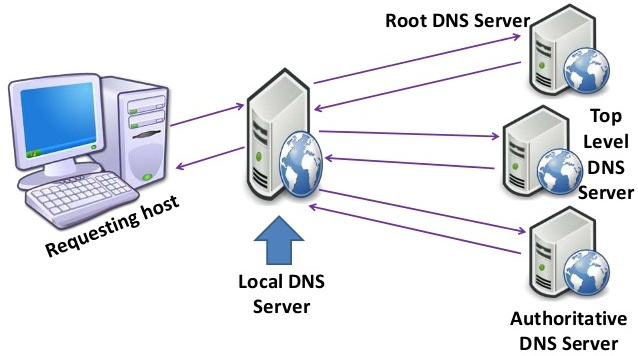
\includegraphics[width=0.5\linewidth]{introduction/dnsWork.jpg}
    \caption{How DNS works. Adapted from \cite{blanche2018understandingDNS}. }
    \label{fig:dnsIntro}
\end{figure}

\section{Motivation}

The Domain Name System (DNS) is a vital element of web activity in the age of technology, but malicious actors are increasingly interested in the system. The abuse of DNS for illegal activities such as confusable domains and phishing has raised questions about the integrity and security of the Internet. The severity and frequency of these concerns are highlighted in recent studies, such as the "Study on Domain Name System (DNS) Abuse: Technical Report" by Bayer et al. \cite{bayer2022}, highlighting the importance of more monitoring and mitigation tactics. Not only have significant cases of DNS abuse endangered user security, but they have also damaged the general trust in the digital economy. Users' trust in online services declines as they become more aware of these hazards, necessitating the implementation of mitigation measures to regain confidence and guarantee a secure online experience. According to Hesselman et al. \cite{hesselman2020}, the idea of a "responsible Internet" aims to increase confidence and sovereignty by improving network-level transparency and accountability. Furthermore, Mathew and Cheshire's \cite{mathew2016} study "Trust and Community in the Practice of Network Security" dives into the significance of trust connections and communities in cybersecurity, demonstrating the negative effects of DNS abuse on user trust.

\begin{figure}[H]
    \centering
    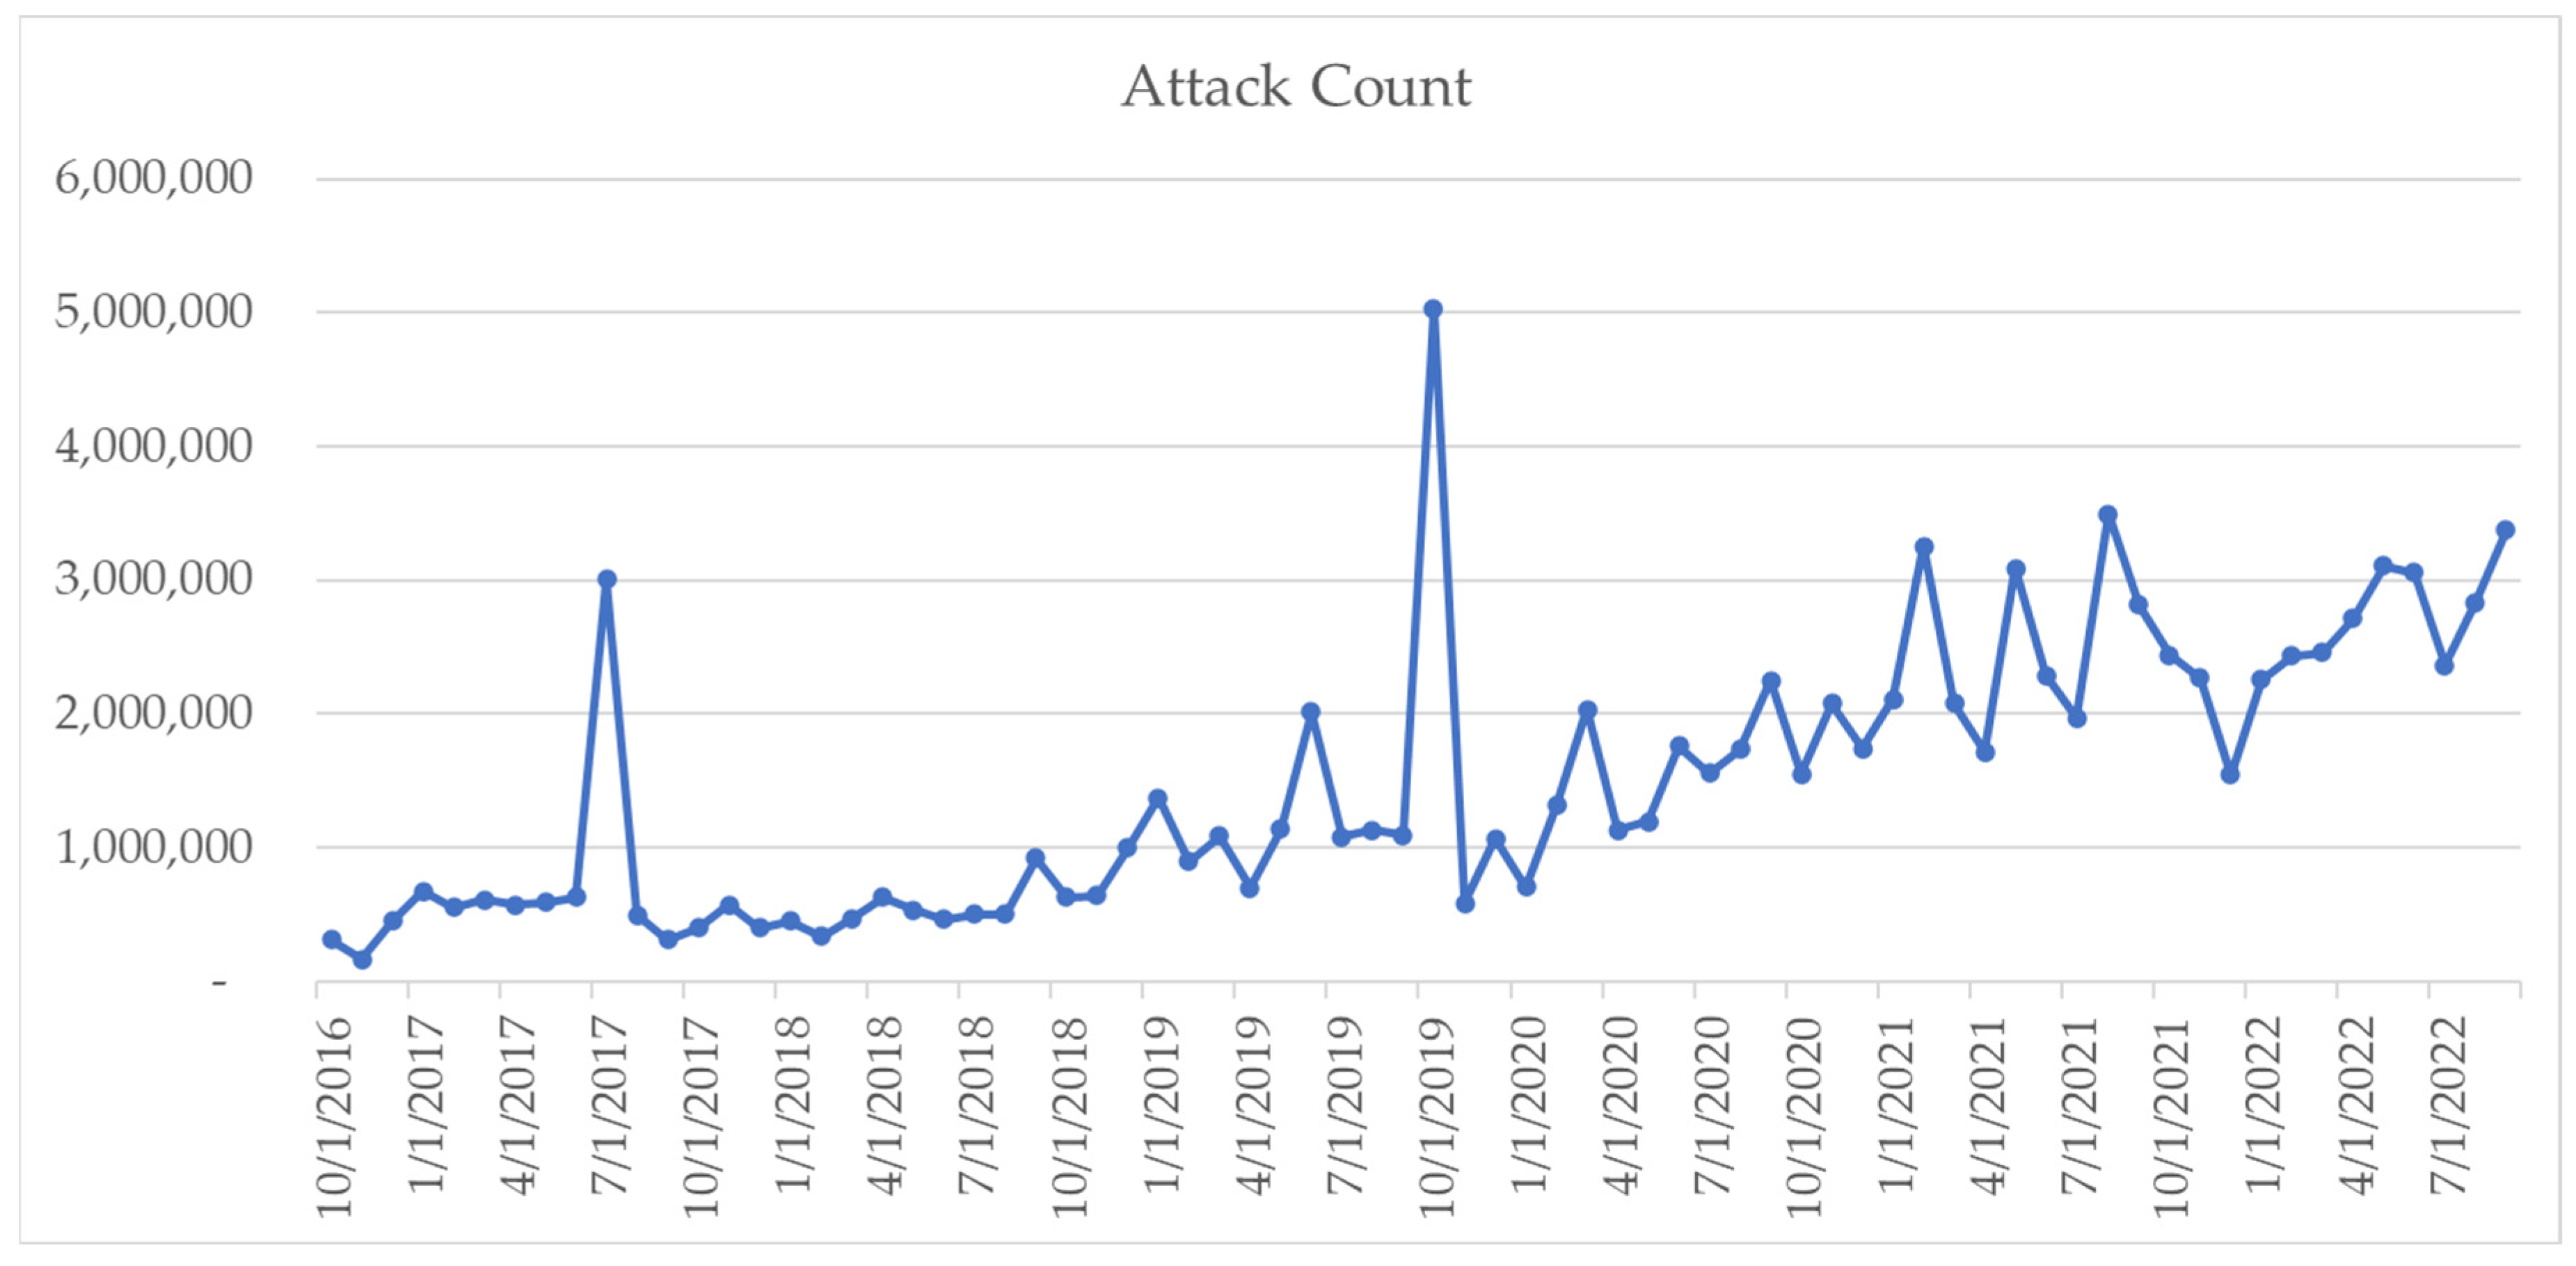
\includegraphics[width=0.9\linewidth]{introduction/maliciousActivity.png}
    \caption{ increase in DNS abuse incidents over time. Adapted from \cite{Rich2023Cyberpsychology}.}
    \label{fig:dnsintro2}
\end{figure}

Organisations are leading the way in this issue, especially DNS infrastructure providers such as registrars and registries. However, their policies and activities tend to not be sufficiently clear. The continuous lack of confidence is made worse by the unclear way in which DNS abuse allegations are handled and the actions that follow. The importance of protecting the Internet and its reliability is recognised in relation to this issue \cite{cerf2022}. These difficulties are compounded by the average user's short attention span and diminished ability to comprehend information, as demonstrated by cognitive psychology studies like Medvedskaya's \cite{medvedskaya2022} investigation of adult Internet users' attention spans. According to this research, consuming digital media may have a detrimental effect on one's capacity for sustained concentration, which would make grasping complicated topics even more difficult. Furthermore, there are ethical and legal consequences to DNS abuse and how to mitigate it in addition to the technical ones. The goal of this project is to close this gap by investigating ways to improve the transparency of DNS abuse mitigation. This study aims to shine light on the present efforts and highlight the obstacles to greater transparency by assessing the current landscape of transparency reports and practices among DNS infrastructure providers. The ultimate objective is to provide a contribution to a system that promotes and enables more efficient and approachable transparency in the mitigation of DNS abuse.


\section{Research Question/Project \& Personal objective} 
\subsection{Research Question}

The primary research question for this project is: "What strategies and practices are registries, registrars, and other parties involved in DNS infrastructure utilising to mitigate DNS abuse, and how do the transparency reports available from these entities characterise and reflect their efforts? Furthermore,how could these practices and reports inform the development of best-practices for transparency in handling DNS abuse complaints?". This question seeks to uncover the mechanisms, policies, and practices in place to mitigate DNS abuse and to what extent these efforts are transparent to the public and stakeholders.

\subsection{Project Objectives}

Assess handling of abuse complaints

\begin{itemize}
  \item Investigate the procedures and policies that DNS infrastructure providers have in place to handle abuse complaints.
  \item Document the types of DNS abuses that are most frequently reported and the response strategies used.
\end{itemize}

Assess Transparency Levels:

\begin{itemize}
  \item Analyse the current state of transparency in the actions taken by providers against DNS abuse.
  \item Identify what information is made public, how it is communicated, and the frequency of disclosure.
\end{itemize}

Benchmark against Best Practices:

\begin{itemize}
  \item Compare the findings with best practices in the industry to identify areas of strength and opportunities for improvement.
  \item Highlight exemplary cases of transparency and effective abuse mitigation.
\end{itemize}

Develop recommendations :

\begin{itemize}
  \item Propose actionable recommendations for DNS infrastructure providers to improve their abuse handling and transparency.
  \item Suggest policy changes or initiatives that could standardise and improve practices in the industry.
  \item Feed into future work on ways in which best practices for transparency could be developed.
\end{itemize}

Contribute to stakeholder understanding: 

\begin{itemize}
  \item Provide insights that help stakeholders, including users, policymakers, and other providers, understand the landscape of DNS abuse handling and transparency.
  \item Offer a foundation for further research and discussion on improving DNS security and trust.
\end{itemize}

\section{Scope}	
The Scope of this project is to perform a detailed examination of the transparency measures taken by registrars and registries to mitigate DNS abuse and to survey registries, registrars, and others involved in mitigating DNS abuse to collect and characterise the transparency reports currently available. In addition to examining current transparency reports to inform future work on ways in which best practices for transparency could be developed. To obtain opinions and insights on current procedures and difficulties, the project will interact with a variety of players in the DNS ecosystem, such as registries, registrars,and policy makers. As part of the research, a set of criteria will also be developed to assess how transparency affects the views of Internet users about trust and safety. It will, however, not include the development of brand-new transparency tools or systems; rather, it will concentrate on examining current procedures and making recommendations for improvements. The main goal of the research is to understand and improve transparency and its impacts. 

\begin{figure}[H]
    \centering
    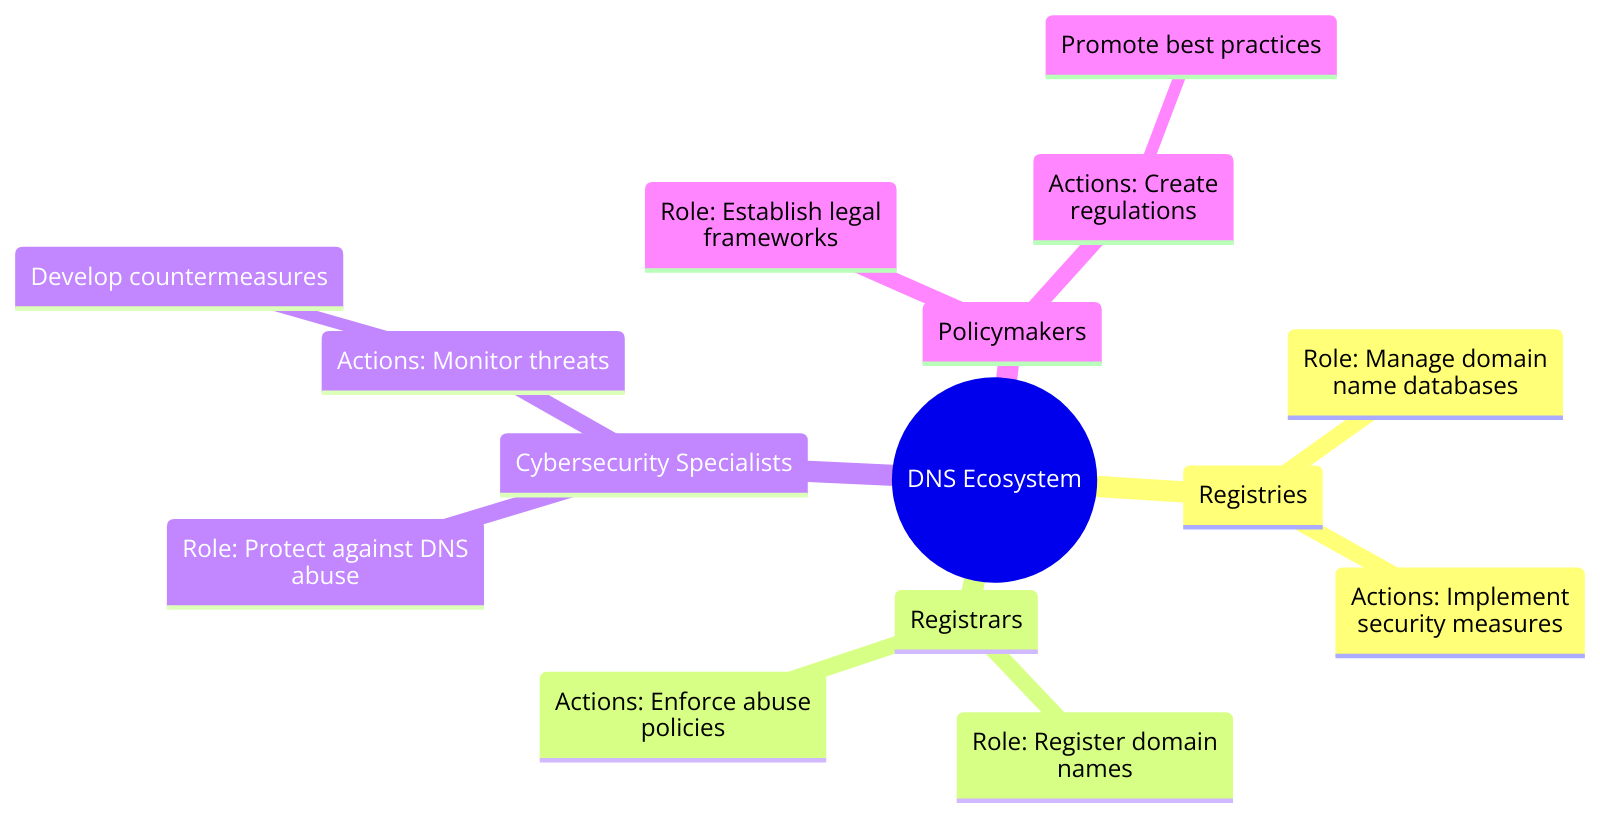
\includegraphics[width=\linewidth]{introduction/diagram (8).png}
    \caption{ DNS ecosystem.}
    \label{fig:dnsintrointro}
\end{figure}

\section{ Outline of the Project Work} 
The goal of this project, "DNS Abuse Transparency," is to better understand and increase the transparency of the efforts of the registrars and registries to mitigate DNS abuse. Research will first examine the different aspects of DNS abuse, such as popular forms like phishing, confusable domains, etc. and their broader consequences. 

Data gathering will be based on a questionnaire that will be distributed to a variety of DNS infrastructure providers and stakeholders throughout the world. The questionnaire attempts to shed light on current practices, the scope and efficacy of transparency measures, and the difficulties encountered in mitigating DNS abuse. At the same time, an examination of the transparency reports currently available from different sources will provide information on the transparency landscape, including the frequency, scope, and accessibility of these reports for users.

Critical evaluation of the handling of DNS abuse reports forms the core of the project. This involves looking at any proactive security measures that may be in place as well as the procedures for dealing with and preventing abusive domain registrations. After that, the research will change its focus to assessing how transparency affects user trust, provider reputation, and the general effectiveness of abuse mitigation techniques.

The project will discover and clarify best practices for transparency in the mitigation of DNS abuse, based on the data and insights obtained. The careful balance between security, privacy, and transparency will be taken into account by these best practices. The project will produce a series of practical suggestions for DNS infrastructure providers based on these findings, with the goal of improving transparency and, consequently, security and confidence in the digital ecosystem.

The project is designed to take place in a sequence of phases, each characterised by deliverables. A comprehensive timeline will guide the progress, guaranteeing an organised and exhaustive study of the subject. Upon completion, this project will have contributed a collection of recommendations and considerations for future study and policy creation in this area of Internet governance, in addition to offering a comprehensive understanding of the current state of DNS abuse transparency.

\section{Outline of the report}

This report offers a comprehensive account of the steps performed, decisions made, and research carried out during the project's development. The format of the report is as follows:

\textbf{Chapter 2 - Background }

This chapter examines the foundations of DNS , along with its significance, weaknesses, and several types of abuse. Observe the tactics and alliances used to combat DNS abuse, including the work of ICANN and the DNS Abuse Institute. The topic of DNS abuse is discussed along with its effects on users and potential risks in the future, with a focus on mitigation techniques and recommended practices.

\textbf{Chapter 3 -  State of the art }

This chapter critically analyses current strategies for DNS abuse mitigation and evaluates their effectiveness. Explores the complex relationship that exists between international governments and DNS, highlighting efforts to openness made by companies such as Google and Cloudflare. In addition to stressing the difficulties in striking a balance between user privacy and compliance requirements, the chapter emphasises the importance of DNS in internet governance. It investigates how various tactics are used and their effects on the larger online ecosystem through critical analysis.

\textbf{Chapter 4 -  Research methodology }

This chapter describes techniques to investigate DNS abuse and transparency from the infrastructure provider. The author goes on how the questionnaires were made, how the responses from stakeholders were analysed, and what kinds of DNS abuse were found. This chapter describes the methodology used to collect and examine data to understand DNS abuse reporting procedures and transparency policies.

\textbf{Chapter 5 -  Implementation }

This chapter involves the practical application, which involves findings from the project, especially the integration of the system, the back-end, the front-end implementations, and the technologies that comprise it. It includes how DNS data on abuse are visualised and the solution to the challenges during the implementation of the system. This part also includes testing and validation to ensure the success of the project.

\textbf{Chapter 6 -  Evaluation \& Discussion }

This chapter assesses how well the project addresses DNS abuse mitigation and improves transparency. Assesses the advantages of transparency in mitigating DNS abuse, as well as the security risks involved. The chapter also addresses the research limits and the degree to which the project's goals were achieved.

\textbf{Chapter 7 -  Conclusion }

This chapter summarises the project's results and recommendations to enhancing DNS abuse mitigation transparency. Consider the difficulties faced, the importance of continuous attempts to improve DNS security, and the possibilities for further study in this field. In conclusion, the importance of cooperation and transparency is emphasised in the fight against DNS abuse. 

\chapter{Background}
\label{Chapt2}
\section{Introduction}

This chapter will explore the fundamental information relevant to this project, with an emphasis on the world of DNS abuse and transparency. It will include a thorough investigation of the domain name system (DNS), its function in the online community, and the variety of abuses it faces , the history of widely used policies and organisations aimed at mitigating DNS abuse, including a thorough examination of the DNS Abuse Institute and its achievements. A 'competition landscape' providing an examination of current market choices, from automated solutions to human tactics, will be provided as we navigate through the current methodology and technology deployed to mitigate DNS abuse. The reader will obtain a detailed understanding of the current situation of DNS abuse and the need for a more open, strong, and proactive strategy by analysing these various techniques and appreciating their strengths and weaknesses. This chapter emphasises the importance of the suggested solution in an era where digital authenticity is required, not only by providing information but also by laying the groundwork for its presentation as a better and essential progression in the battle against DNS abuse.

\section{Understanding DNS \& Its Vulnerabilities}

The Domain Name System (DNS) is a significant part of the infrastructure of the Internet, serving as the key that converts computer-understandable IP addresses into human-friendly domain names. Although the DNS plays a vital role in maintaining ongoing online activities, privacy and security problems still arise. The ScienceDirect paper "Domain Name System Security and Privacy: A Contemporary Survey" provides a detailed analysis of these concerns that highlights the fundamental importance of DNS while illuminating the weaknesses that malicious actors may take advantage of \cite * {Sciencedirect2023dns}. A variety of security threats exist, ranging from DNS infrastructure-targeting distributed denial-of-service (DDoS) assaults to cache poisoning and hijacking. Each of these attacks has the potential to do significant harm, including interruptions in service and the promotion of theft and spying. Due to the standard DNS design's lack of encryption, users' query data is vulnerable to abuse and eavesdropping, raising serious privacy problems. However, weaknesses do not mark the end of the story. In the same survey, new approaches are examined to improve DNS security and privacy. The use of DNSSEC (DNS Security Extensions), which authenticates DNS data and guarantees its integrity while repelling some types of attack, is one example of these advances in security measures. In addition, privacy-enhancing technologies are being used to encrypt DNS queries, preventing eavesdropping and manipulation, such as DNS over HTTPS (DoH) and DNS over TLS (DoT). The environment of DNS threats and defences is always changing in sync with the Internet. For systems to be robust and resilient, it is essential to understand these weaknesses and the continuous efforts being made to mitigate them. An in-depth discussion of DNS vulnerability details, the effects of these safety concerns, and creative solutions that aim to bring in a new era of DNS security and privacy will be provided in this section.

In a usual DNS lookup, three kinds of queries come into play to streamline the process and minimise the data journey. The first type is a recursive query, where the DNS client expects a direct answer or an error if the record cannot be found from the DNS server. Then there's an iterative query, which means if the server doesn't have the answer, it points the client to another server that might know, and the client keeps asking down the line until it gets an answer or hits a dead end. Lastly, a non-recursive query happens when the DNS server already knows the answer either because it is directly responsible for that piece of information or it has it saved from earlier inquiries. This method helps in reducing unnecessary internet traffic and lightening the load on the servers involved.

\section{Strategies \& Collaborations in Addressing DNS Abuse}

The DNS Abuse Institute, which will focus on DNS abuse to help in increasing safety and security through the domain name system, is going to be cantered on these efforts to address DNS abuse with a comprehensive approach throughout the infrastructure of the internet. It helps the internet community in the identification, reporting, and mitigation of DNS abuse in its mission to make the online environment more secure. Efforts by the institute, such as Compass Dashboards, provide vital data to registries and registrars that will enable proper decisions on combating DNS abuse. They show the commitment to transparency and education by issuing publications such as the "DNSAI 2022 Annual Report" or "DNSAI Bulletin 2023 04; Account Takeovers," which provide information on DNS abuse and how recommended mitigation practices \cite{dnsabuseinstitute2023}. Another such global strategy against DNS abuse has been contributed by the Internet Corporation for Assigned Names and Numbers (ICANN)\cite{icann2022dnsabuse} in collaboration with the entire DNS community, ICANN supports a synchronised method in the development of policies and standards on how to mitigate DNS abuse while ensuring the openness of the Internet. These participatory pillars hint at concerted efforts through policy development, technological developments, and stakeholder engagement as a central component in this collective approach to combating DNS abuse \cite{dnsai2022report}. 



\section{Different Forms of DNS Abuse}

DNS abuse takes many forms, each with its procedures and effects on users and the Internet as a whole. It is essential to understand these various pieces of evidence to create responses and regulations that work. This section will examine the comprehensive analysis of DNS abuse as presented, going into the description, mechanism, and impact of each kind \cite{dotmagazine2022dnsabuse}.

\subsection{Phishing}
\begin{itemize}
    \item \textbf{Description:} Phishing is a technique aimed at deceiving individuals by creating website addresses that mimic those of companies, to trick users into revealing sensitive information such as login credentials, credit card numbers, or personal identification information \cite{webinarcare2023dnsstats}.
    \item \textbf{Mechanism:} This deception often occurs through emails or messaging services that direct users to websites similar to authentic ones \cite{jakobsson2006phishing}.
    \item \textbf{Impact:} Victims may suffer identity theft, financial fraud, and security compromise.
\end{itemize}

\subsection{Confusable Domains (Typosquatting)}
\begin{itemize}
    \item \textbf{Description:} Registering domain names that look visually similar to popular websites, taking advantage of typing errors or character similarities \cite{inta2023dnstypo}.
    \item \textbf{Mechanism:} Users may accidentally visit these websites when making a typo in a URL, potentially exposing them to malware or phishing attempts.
    \item \textbf{Impact:} Deception of users and potential harm to brand reputation \cite{edelman2008typosquatting}.
\end{itemize}

\subsection{Domain Hijacking}
\begin{itemize}
    \item \textbf{Description:} Unauthorised acquisition of domain names by exploiting security vulnerabilities in the domain registration system \cite{inta2023dnstypo}.
    \item \textbf{Mechanism:} Attackers may use tactics like social engineering, phishing, or exploiting security loopholes to gain control over a domain.
    \item \textbf{Impact:} Loss of website control, redirection to malicious sites, and potential data breaches.
\end{itemize}

\subsection{Botnets}
\begin{itemize}
    \item \textbf{Description:} Botnets involve controlling a group of computers infected with malware, used to carry out attacks or spread spam and malware \cite{citpyour}.
    \item \textbf{Mechanism:} Malware infects computers of unsuspecting users, incorporating them into a network under the attacker's control.
    \item \textbf{Impact:} Can result in large-scale DDoS attacks, mass spam campaigns, and widespread malware dissemination.
\end{itemize}

\subsection{Fast Flux Hosting}
\begin{itemize}
    \item \textbf{Description:} A technique used to conceal the location of websites associated with phishing and malware distribution \cite{lin2013genetic}.
    \item \textbf{Mechanism:} Involves a network of compromised hosts that regularly modify DNS records to evade detection.
    \item \textbf{Impact:} Makes tracking and shutting down malicious sites difficult.
\end{itemize}

\subsection{Domain Generation Algorithms (DGA)}
\begin{itemize}
    \item \textbf{Description:} DGAs generate domain names that act as meeting points for botnets \cite{antonakakis2012throw}.
    \item \textbf{Mechanism:} Malicious software uses algorithms to generate a sequence of domain names for command-and-control servers.
    \item \textbf{Impact:} Adds complexity to efforts to disrupt botnet command and control channels.
\end{itemize}
\captionsetup{font= footnotesize}
\begin{figure}[H]
\centering
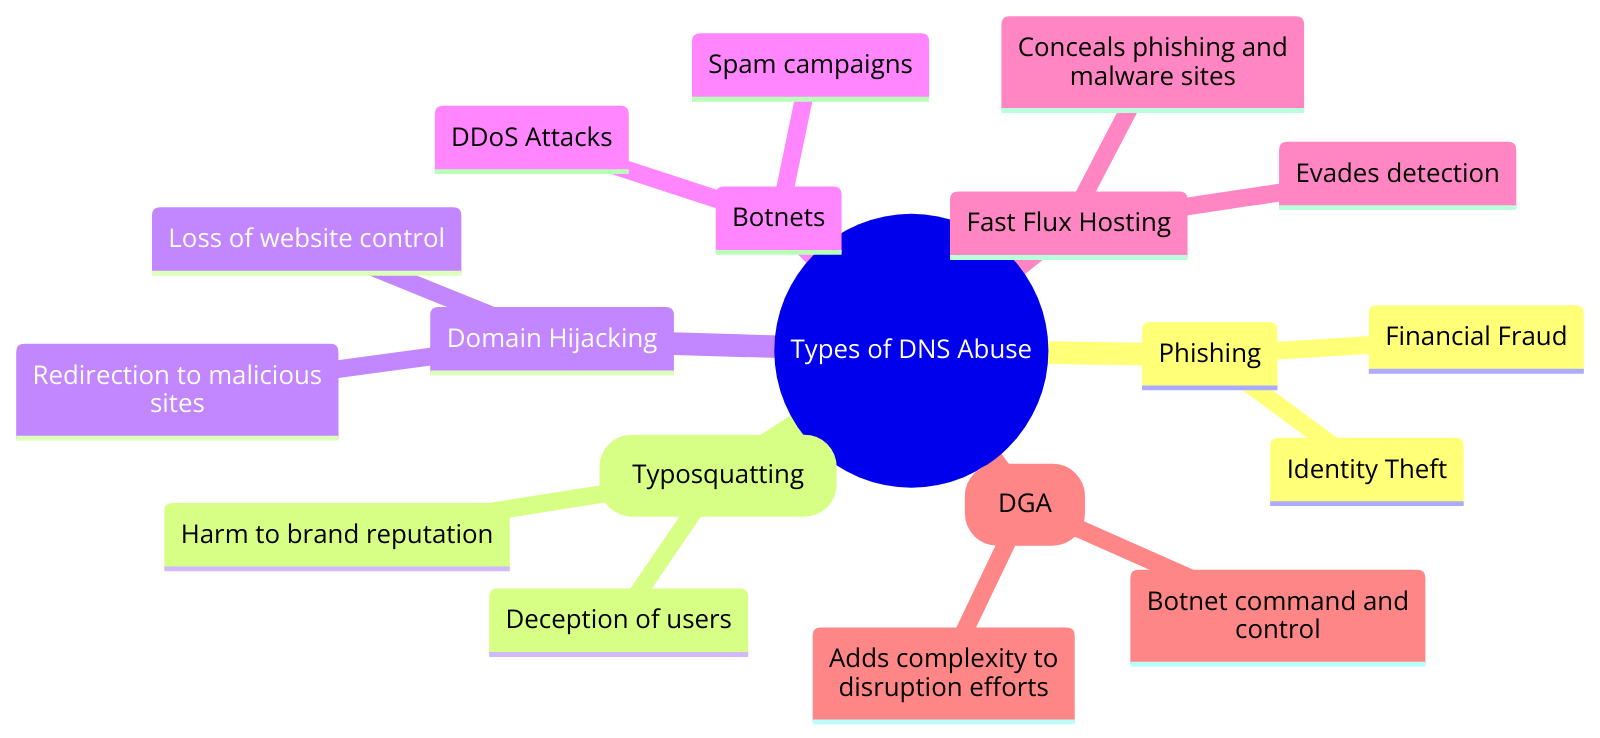
\includegraphics[width=1.0\textwidth]{background/DNSabuseForms.png}
\caption{Impact of DNS Abuse}
\label{fig:figureThree}
\end{figure}



\section{How DNS Abuse Harms Users}

DNS abuse has serious and detrimental effects for both users and organisations, going beyond basic technological disruptions. Identity theft is among the most direct and direct effects. Phishing attacks, a frequent type of DNS abuse, use realistic websites to trick visitors into revealing sensitive data. Such attacks can produce information that results in financial theft, unauthorised access to accounts, and long-term damage to a person's reputation and credit \cite{godaddy2023dnsabuse}.

\subsection{Identity Theft}
\begin{itemize}
    \item \textbf{Phishing:} Phishing attacks often use domain names that imitate legitimate websites, fooling users into providing sensitive information such as usernames, passwords, or financial details, leading to potential identity theft.
\end{itemize}

\subsection{Financial Loss}
\begin{itemize}
    \item \textbf{Deceptive Transactions:} Users may be tricked into making payments to deceptive websites or unknowingly disclose their credit card information, resulting in financial losses \cite{bohme2013economics}.
\end{itemize}

\subsection{Data Breach}
\begin{itemize}
    \item \textbf{Malware:} Malicious software spread through compromised DNS systems can allow unauthorised access to corporate data, leading to data breaches \cite{fowler2016data}.
\end{itemize}

\subsection{System Compromise}
\begin{itemize}
    \item \textbf{Malware Infection:} Systems infected with malware due to DNS abuse can be exploited for further attacks, including the creation of botnets or the distribution of ransomware, resulting in system compromise \cite{saxe2018malware}.
\end{itemize}
\captionsetup{font= footnotesize}
\begin{figure}[H]
\centering
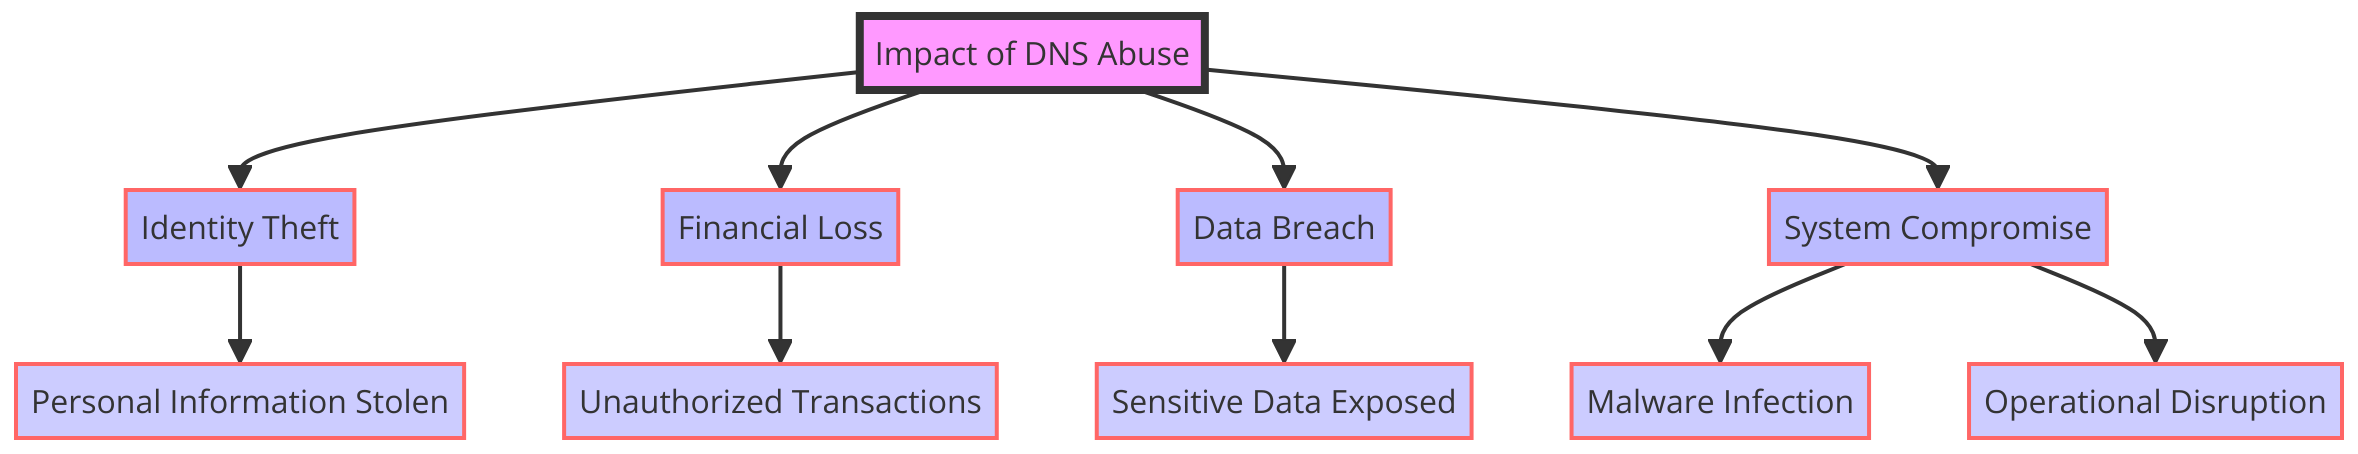
\includegraphics[width=1.0\textwidth]{background/DNSabuseHarm.png}
\caption{Different Forms of DNS Abuse}
\label{fig:figureFour}
\end{figure}


\section{Future Dangers of DNS Abuse}

As technology develops, so do bad actor strategies and tools, creating a dynamic environment for DNS abuse that could present new risks in the future. The sophistication of attacks has increased, which is a major issue. Bad actors are always creating increasingly sophisticated methods to take advantage of DNS, such as creating more convincing phishing schemes and using advanced virus distribution networks \cite{icann2022dnsabusetrends}.

\subsection{Increased Sophistication}
\begin{itemize}
    \item \textbf{Evolving Techniques:} Bad actors are constantly developing more sophisticated techniques to exploit DNS, such as advanced phishing schemes and malware distribution \cite{wrightson2014advanced}.
\end{itemize}

\subsection{IoT Vulnerabilities}
\begin{itemize}
    \item \textbf{Expanding Vulnerabilities:} The widespread adoption of Internet of Things (IoT) devices, which often lack robust security measures, presents a growing target for DNS-based attacks \cite{mahmoud2015internet}.
\end{itemize}

\subsection{Infrastructure Attacks}
\begin{itemize}
    \item \textbf{DNS as a Prime Target:} Attacks on DNS infrastructure can disrupt internet services on a large scale, including DDoS attacks targeting DNS providers or exploiting weaknesses in DNS protocols \cite{dooley2017dns}.
\end{itemize}

\subsection{Deepfakes \& AI}
\begin{itemize}
    \item \textbf{AI-Enhanced Phishing:} The use of AI technologies, such as deepfakes, has made phishing attacks more convincing and deceptive, manipulating audio and video content to impersonate trusted entities \cite{schick2020deep}.
\end{itemize}

\subsection{Cloud Computing Vulnerabilities}
\begin{itemize}
    \item \textbf{Targeting Cloud Services:} As organisations increasingly rely on cloud-based services, bad actors are exploiting DNS vulnerabilities to attack these platforms, potentially leading to data breaches and service disruptions \cite{mather2009cloud}.
\end{itemize}

\subsection{Mobile Device Exploitation}
\begin{itemize}
    \item \textbf{Mobile DNS Attacks:} The rising usage of mobile devices has led bad actors to target smartphones and tablets through DNS-based attacks, which can lead to data theft and the spread of malware \cite{au2016mobile}.
\end{itemize}

\subsection{Cryptocurrency \& Blockchain Exploitation}
\begin{itemize}
    \item \textbf{Crypto-Related DNS Attacks:} Attackers could exploit DNS vulnerabilities to redirect users to fake cryptocurrency exchanges or blockchain platforms, leading to financial fraud and theft of digital assets \cite{bashir2019advanced}.
\end{itemize}

\subsection{Political and Information Warfare}
\begin{itemize}
    \item \textbf{DNS in Cyber Warfare:} The manipulation of domain name systems can be used to spread misinformation or disrupt services during significant political events, serving as a tool for political and information warfare \cite{chapple2021cyberwarfare}.
\end{itemize}

\subsection{Exploiting Emerging Technologies}
\begin{itemize}
    \item \textbf{Abuse in New Tech Domains:} As new technologies such as 5G, AI, and quantum computing advance, tactics involving DNS abuse are likely to evolve, potentially leading to more sophisticated attacks \cite{brunner2021cybersecurity}.
\end{itemize}

\subsection{Supply Chain Attacks}
\begin{itemize}
    \item \textbf{DNS in Supply Chain Compromise:} DNS manipulation can also be employed as part of supply chain attacks, targeting software updates or cloud-based services to compromise organisations \cite{boyson2014cyber}.
\end{itemize}

By understanding these future dangers and emerging trends, stakeholders can better prepare and adapt their strategies to anticipate and counteract the evolving nature of DNS abuse.


\captionsetup{font= footnotesize}
\begin{figure}[H]
\centering
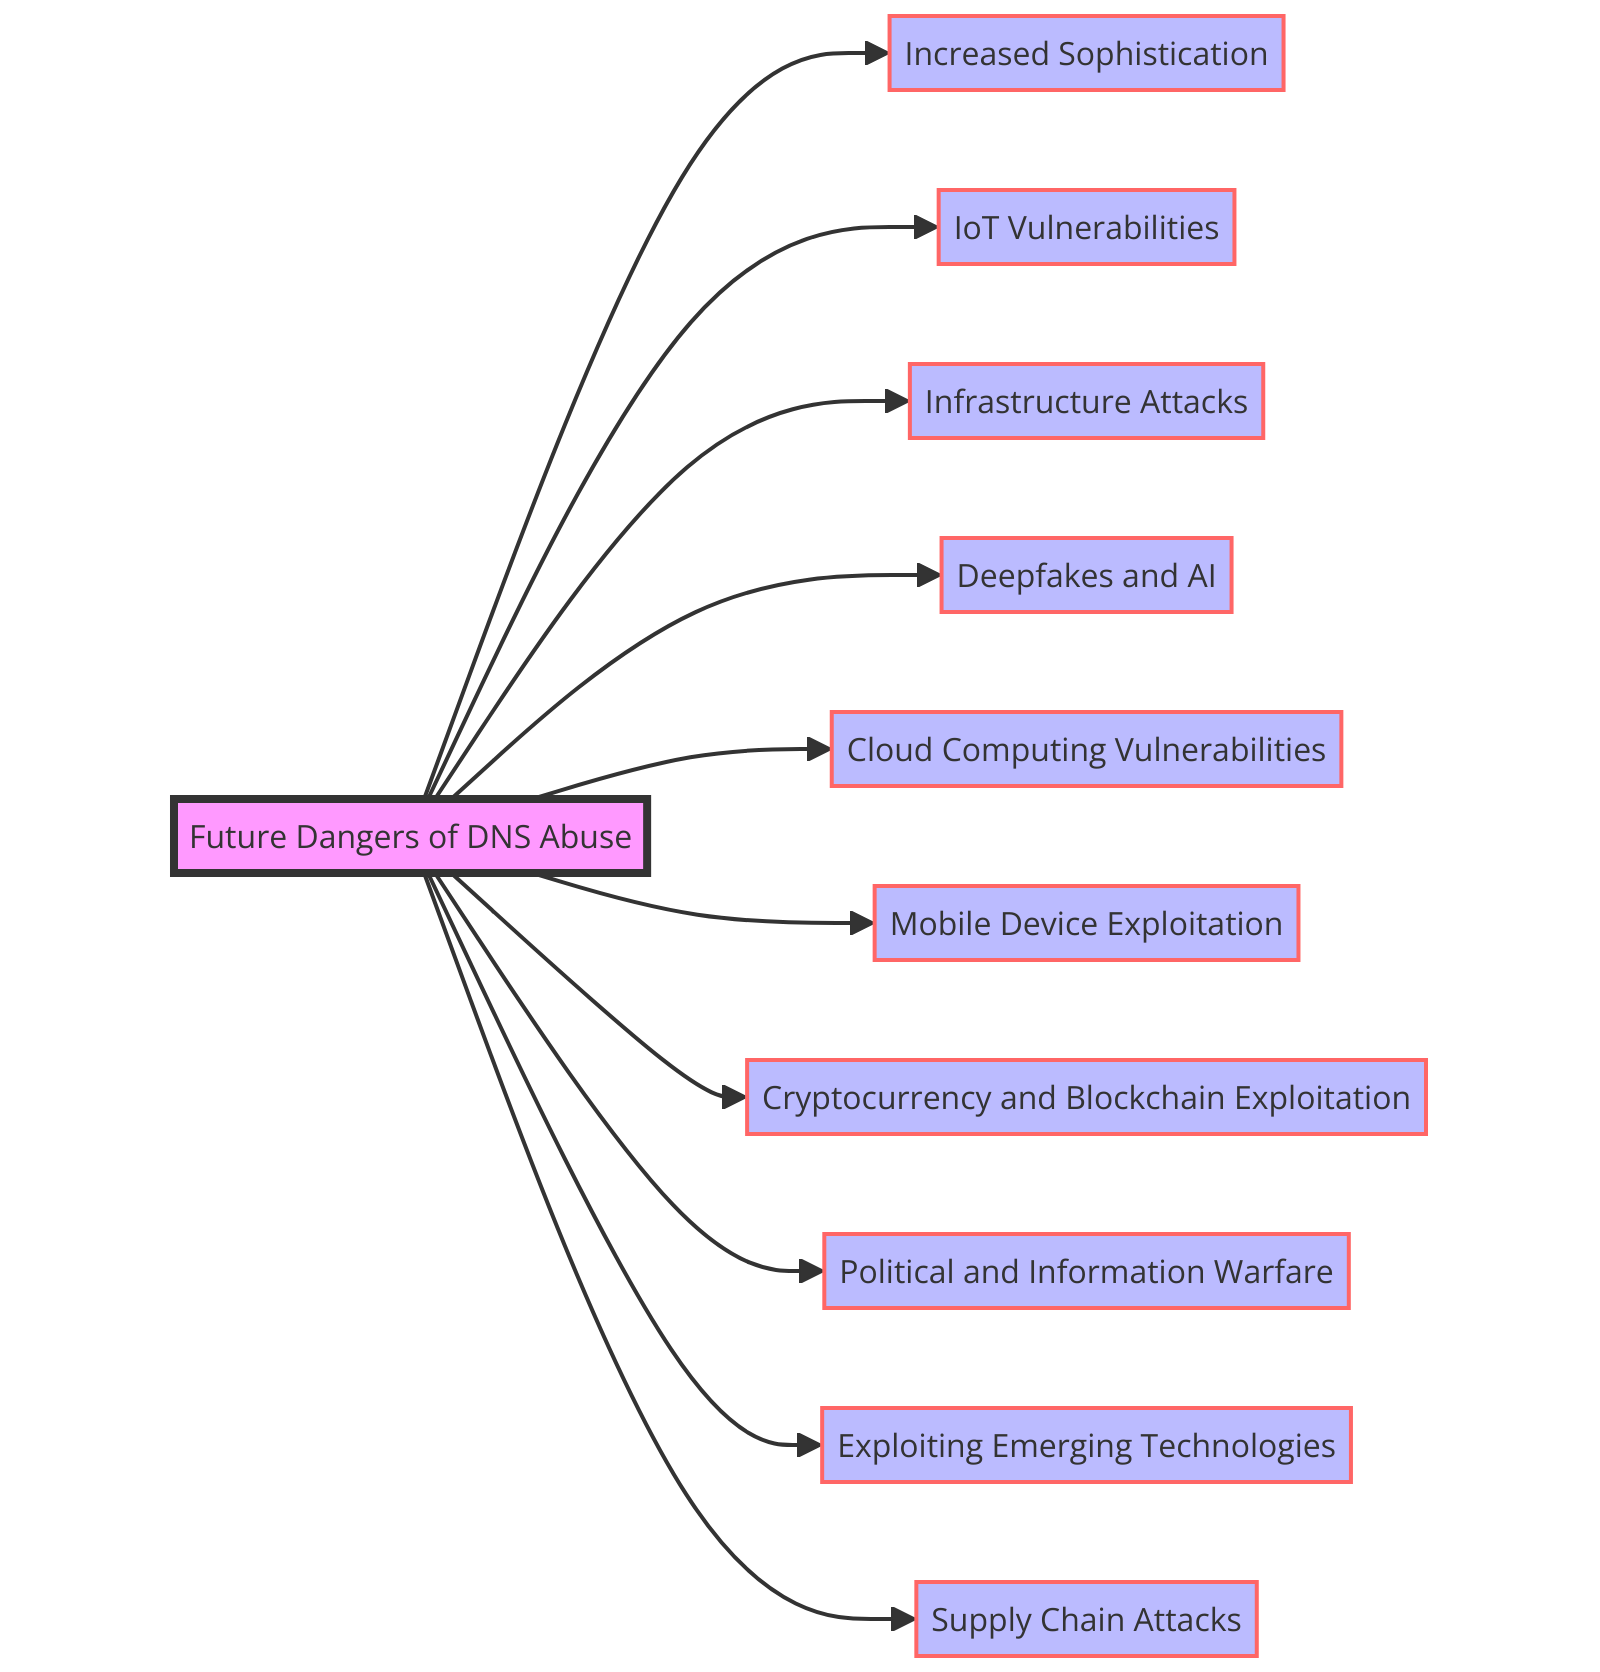
\includegraphics[width=1.2\textwidth]{background/DNSfutureDanger.png}
\caption{Future dangers of DNS abuse}
\label{fig:figureFive}
\end{figure}
\newpage


\section{Foundational Mitigation Strategies \& Best Practices }

To address the broad nature of the threats, mitigating DNS abuse requires an integrated strategy that integrates multiple strategies and best practices. Setting up procedures for reporting and monitoring is one fundamental tactic. Automated systems have the ability to track domain name registration patterns that may indicate DNS abuse, and protocols to report questionable actions can help ensure prompt intervention \cite{icannndnssec}. To confirm security and ensure that the systems have not been compromised, regular audits of DNS configurations and domain registrations are also necessary \cite{lucas2021tls} .

\begin{enumerate}
    \item \textbf{Monitoring \& Reporting}
    \begin{itemize}
        \item Implementation: Use automated systems to monitor the registration of domain names for patterns that may indicate DNS abuse \cite{icannndnssec}. Establish procedures for reporting activities to authorities or cybersecurity organisations \cite{lucas2021tls}.
    \end{itemize}
    \item \textbf{Security Awareness Training}
    \begin{itemize}
        \item Implementation: Develop training programs for users and IT staff with a focus on recognising phishing attempts, practising browsing habits, and understanding DNS security.
    \end{itemize}
    \item \textbf{DNS Security Extensions (DNSSEC)}
    \begin{itemize}
        \item Implementation: Deploy DNSSEC to ensure the integrity of DNS data. This involves signing DNS records to protect against modifications and DNS spoofing.
    \end{itemize}
    \item \textbf{Multi-Factor Authentication (MFA)}
    \begin{itemize}
        \item Implementation: Enforce multi-factor authentication (MFA) for domain registrars and interfaces used to manage DNS \cite{icannndnssec}. This adds a layer of security beyond passwords, helping to prevent unauthorised domain transfers or alterations \cite{moghaddam2014ecco}.
    \end{itemize}
    \item \textbf{Blacklisting \& Takedown Services}
    \begin{itemize}
        \item Implementation: Collaborate with cybersecurity firms to identify and blacklist domains engaged in malicious activities. Establish response teams dedicated to removing domains involved in DNS abuse.
    \end{itemize}
    \item \textbf{Collaboration}
    \begin{itemize}
        \item Implementation: Foster collaboration among internet service providers (ISPs), domain registrars, governments, and cybersecurity organisations. Share intelligence and best practices to collectively enhance defense against DNS abuse \cite{skopik2017collaborative}.
    \end{itemize}
    \item \textbf{Regular Audits}
    \begin{itemize}
        \item Implementation: Conduct security audits of domain registrations and DNS configurations to verify their security and ensure they have not been compromised \cite{coronado2014auditing}.
    \end{itemize}
    \item \textbf{Machine Learning}
    \begin{itemize}
        \item Implementation: Using AI and machine learning algorithms to analyse patterns in DNS traffic and proactively predict instances of DNS abuse \cite{icannndnssec}. This proactive approach enables the identification of threats before they materialise \cite{tsukerman2019machine}.
    \end{itemize}
    \item \textbf{Geo-Blocking \& IP Filtering}
    \begin{itemize}
        \item Implementation: Deploy geo-blocking and IP filtering techniques to limit access to DNS services from regions that have a history of DNS abuse. This can reduce the risk that attackers will use these services to carry out malicious activities or distribute malware \cite{meeseedited}.
    \end{itemize}
    \item \textbf{Enhanced Domain Validation Procedures}
    \begin{itemize}
        \item Implementation: Enhance the domain registration process by implementing validation procedures. This may involve verifying the identity of individuals or organisations that register domains, especially domains that resemble brands or fall into sensitive categories. By taking these measures, we can strengthen security and mitigate risks associated with fraudulent domain registrations.
    \end{itemize}
\end{enumerate}

Each of these strategies plays a role in creating a comprehensive defence against DNS abuse. By integrating these tactics, organisations can establish robust, proactive measures to detect, prevent, and mitigate the ever-evolving threats posed by DNS abuse.

\captionsetup{font= footnotesize}
\begin{figure}[H]
\centering
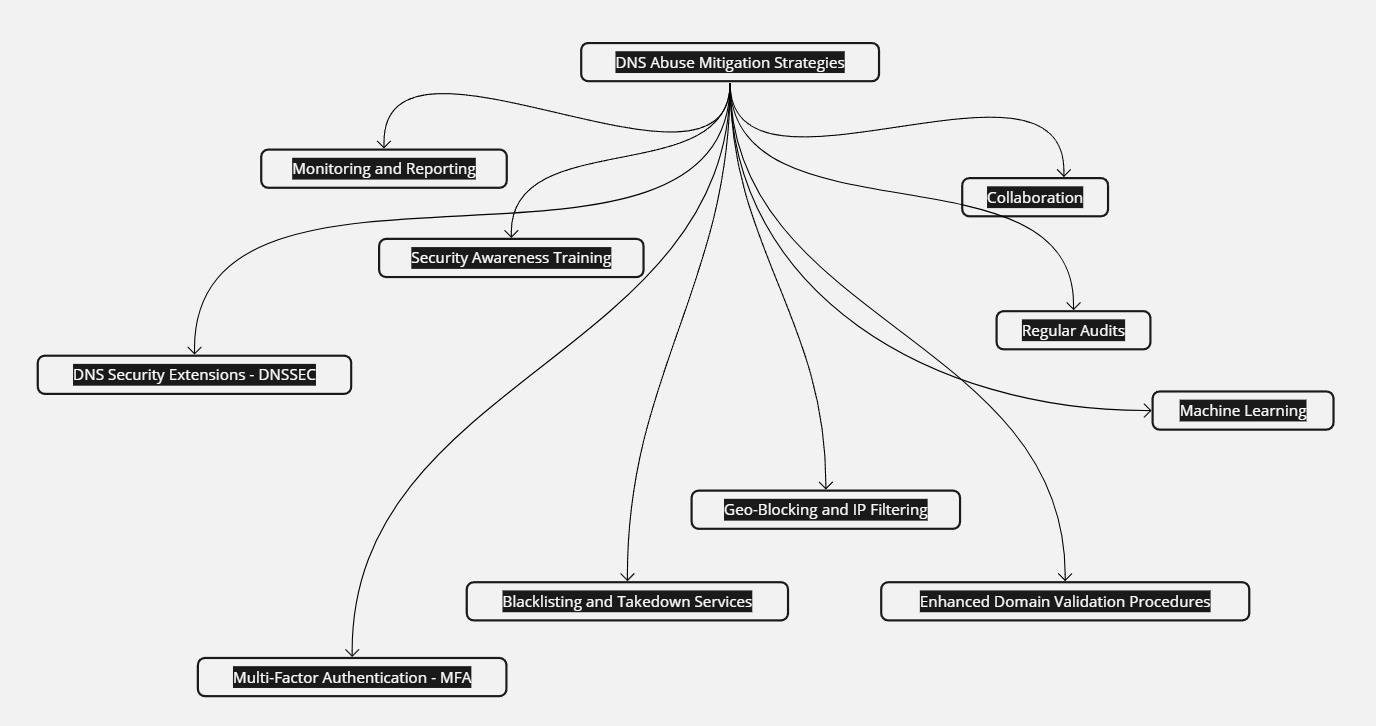
\includegraphics[width=0.7\textwidth]{background/DNSabuseMiti.jpg}
\caption{Future dangers of DNS abuse}
\label{fig:figureSix}
\end{figure}




\section{Summary \& Synthesis}

After exploring the different forms of DNS abuse , How DNS abuse harms user , Future Dangers of DNS abuse and Mitigation Strategies and Best Practices. I have designed a table that has DNS abuses and the best possible mitigation strategies to help them against them, taking into account the transparency story behind it , user harm and reasoning. 

{
\footnotesize

\begin{longtable}{|p{2.5cm}|p{2.5cm}|p{4cm}|p{3cm}|p{4cm}|} 

\hline
\textbf{DNS Abuse } & \textbf{User Harm} & \textbf{Mitigation Strategy} & \textbf{Reasoning} & \textbf{Transparency Aspect} \\ \hline
\endfirsthead

\multicolumn{5}{c}%
{
\hline \textbf{DNS Abuse} & \textbf{User Harm} & \textbf{Mitigation Strategy} & \textbf{Reasoning} & \textbf{Transparency Aspect} \\ \hline
\endhead

\hline \multicolumn{5}{|r|}{{Continued on next page}} \\ \hline
\endfoot

\hline
\endlastfoot
Phishing & \mbox{Identity Theft}, Financial Loss &  \mbox{Security Awareness} \mbox{Training, Enhanced Domain} Validation Procedures & \mbox{Training helps users} \mbox{recognize phishing} \mbox{attempts. Validation} prevents registration of mimic domains. & \mbox{Increases awareness and} \mbox{scrutiny during domain} registration. \\ \hline

\mbox{Confusable} Domains \mbox{(Typosquatting)} & Unauthorised Account Access & \mbox{Enhanced Domain} \mbox{Validation Procedures}, Regular Audits & \mbox{Prevents Registration} of Similar Domains. \mbox{Audits ensure} \mbox{compliance.} & \mbox{transparent domain} \mbox{registration process.} \\ \hline

\mbox{Domain} \mbox{Hijacking} & \mbox{System} \mbox{Compromise}, \mbox{Data Breach} & \mbox{Multi-Factor Authentication} (MFA), Regular Audits & \mbox{MFA secures domain} management. \mbox{Audits verify security} measures. & \mbox{Accountability in domain} management. \\ \hline

Botnets & \mbox{Malware} \mbox{Distribution} & Collaboration,Machine Learning & \mbox{Intelligence Sharing} \mbox{identifies botnet} \mbox{activities. AI predicts} \mbox{the formation of} \mbox{botnets}. & \mbox{Shared responsibility and} proactive detection. \\ \hline

\mbox{Fast Flux} \mbox{Hosting} & \mbox{System Infections} & Blacklisting and Takedown Services, Geo-Blocking & \mbox{Rapid response to} \mbox{malicious domains.} Restrict access from risky regions. & Responsive and transparent threat management. \\ \hline

\mbox{Domain} \mbox{Generation} Algorithms (DGA) & \mbox{Malware} \mbox{Distribution} & \mbox{Machine Learning, DNS} \mbox{Security Extensions} (DNSSEC) & AI detects abnormal \mbox{patterns. DNSSEC} \mbox{prevents spoofing.} & Integrity and trust in DNS data. \\ \hline

\mbox{IoT} \mbox{Vulnerabilities} & \mbox{Unauthorised} \mbox{Access, Data} \mbox{Breach} & \mbox{Security Awareness} \mbox{Training, Collaboration} & \mbox{Educates on security} \mbox{practices.} \mbox{Collaboration on best} \mbox{practices.} & \mbox{Open exchange of} \mbox{knowledge and efforts.} \\ \hline

Infrastructure Attacks & \mbox{DDoS Attacks}, \mbox{System Downtime} & DNSSEC, Collaboration & Protects DNS data integrity. Sharing of threat intelligence. & \mbox{Collective action}  \mbox{strengthens the DNS} infrastructure.  \\ \hline

Deepfakes and AI & \mbox{Identity Theft}, \mbox{Misinformation} & \mbox{Security Awareness} \mbox{Training, Monitoring} & \mbox{Recognising Phishing.} \mbox{Monitor} \mbox{AI threats.} & \mbox{Vigilance and prompt} \mbox{threat reporting.} \\  \hline

\mbox{Cloud} \mbox{Computing} Vulnerabilities & \mbox{Data Breach}, \mbox{Unauthorised} Access & Regular Audits, Enhanced Validation & \mbox{Secure DNS settings} \mbox{in cloud services.} \mbox{Prevents exploitation.} & \mbox{Framework for secure} \mbox{domain use in cloud.} \hline

\mbox{Mobile Device} Exploitation & Unauthorised Access, Financial Loss & \mbox{MFA, Security Awareness} Training & \mbox{Secures account} \mbox{access.} \mbox{ Raises awareness} of threats. & Mobile security awareness and protection. \\ \hline

\mbox{Cryptocurrency} \mbox{and Blockchain} Exploitation & \mbox{Financial Theft}, \mbox{Account} \mbox{Compromise} & \mbox{Enhanced Validation}, \mbox{Collaboration} & \mbox{Prevents fraudulent} \mbox{domain registrations.} \mbox{Collaboration on} \mbox{threat intelligence.} & Security registration and defence of domains. \\ \hline

\mbox{Political and} Information Warfare & Misinformation, Political \mbox{Manipulation} & Monitoring, Collaboration & \mbox{Monitoring abuse in} \mbox{campaigns. Unified} \mbox{response to } \mbox{misinformation.} & Transparency in monitoring and collective action. \\ \hline

\mbox{Exploiting} Emerging \mbox{Technologies} & System \mbox{Vulnerabilities} &\mbox{ Machine Learning,} \mbox{Collaboration} & \mbox{Analytics to predict} \mbox{DNS abuse. Share} \mbox{knowledge about} \mbox{threats.} & \mbox{Innovation in defense}  \mbox{strategies and sharing.} \\ \hline

\mbox{Supply Chain} \mbox{Attacks} & \mbox{System} \mbox{Compromise,} Data Breach & Regular Audits, Blacklisting & \mbox{Audits for DNS} \mbox{integrity. Rapid} \mbox{response to threats.} & \mbox{Transparency in supply} \mbox{chain security.} \\ \hline

\caption{Mitigation Strategies Against DNS Abuse and Their Impact on Users} 

\end{longtable}

}

Finally , This chapter has examined all aspects of DNS abuse,  the various forms, the serious harm it does, as well as potential future threats and new trends. To create efficient regulations and countermeasures, it is essential to understand the extent and consequences of DNS abuse. The conversation emphasised DNS's vital function in the digital ecosystem as well as its susceptibility to abuse. Significant progress towards resolving these issues has been made by organisations like the DNS Abuse Institute and ICANN, as well as developments in DNS privacy and security technologies like DoT and DoH. However, as new technologies are incorporated into the equation and the threat environment changes in sophistication, it becomes increasingly important to adopt alert, flexible, and cooperative strategies.  

The mitigation techniques and best practices discussed in this chapter provide a roadmap for mitigating DNS abuse. Every tactic contributes to a defence mechanism, from advanced technology solutions and improved methods for validation to monitoring and reporting. It is impossible to overestimate the value of cooperation, regular checks, and the application of cutting-edge technologies to anticipate and mitigate DNS abuse. After analysing the data, it is evident that a team effort is needed to comprehend, track, and mitigate DNS abuse. A complex strategy that integrates multiple techniques and encourages collaboration across industries is required instead of a single, insufficient strategy. Our approaches to preserving the integrity and security of the DNS and, consequently, the larger internet infrastructure must adapt, as does the digital environment.

By understanding the connections between different aspects of DNS abuse and reinforcing the collective effort required for effective mitigation, stakeholders can be better prepared to face the challenges ahead. This chapter sets the stage for further research and action, with the aim of contributing to a safer and more secure digital world.



\chapter{State of the Art}

This chapter explores the strategies used to mitigate DNS abuse and new developments in this field. Explore and evaluate the effectiveness and transparency of multiple mitigation techniques, including DNS filtering and threat intelligence in which information about cyber attacks is organised and analysed by experts. Additionally, the use of domain-generating techniques and DoT and DoH are two novel forms of DNS abuse that are highlighted in this section. Along with the role of AI and machine learning in identifying and mitigating DNS abuse is covered. The final half of the section includes a discussion on potential future research areas and technologies to improve DNS abuse mitigation. Case studies offer practical insights into DNS abuse occurrences. 


\section{Current Strategies and Their Effectiveness in Relation to DNS Abuse}


DNS abuse presents a significant challenge for internet entities involved in domain name management. Various approaches are employed to mitigate such abuse, including DNS filtering, which regulates access to specific websites and prevents you from accessing malicious sites that can administer phishing and ransomware. Additionally, threat intelligence methodologies leverage data analysis to identify potential risks, as exemplified by \cite{schmid2021thirty}. Anomaly detection plays a role in identifying suspicious DNS activities indicative of malicious intent using Packet Analysis to analyse individual packets for DNS allowing for real-time detection and statistical analysis, which involves performing statistical analysis on a large dataset of DNS traffic. However, these methods can face operational challenges, such as errors and the need for fast access to critical threat data. 

\subsection{Transparency in DNS Abuse Mitigation \& DNS Relevance}

\begin{enumerate}
    \item A Case Study of Cloudflare's Transparency Approach


Cloudflare is firmly committed to transparency \cite{cloudflare_transparency_2022}, the cornerstone of its relationship with customers, which guides its approach to DNS abuse reports and requests that may come from law enforcement. This shaves their actions and policies to mould a trustworthy environment while addressing internet safety and privacy concerns. Their approach to handling DNS abuse reports and law enforcement requests is grounded in three core principles:

\begin{enumerate}
    \item Require Due Process:  Whatever shall be lawfully requiring due process of law enforcement and Cloudflare shall adhere in letter and spirit. They are neutral in behaviour and do not intend to hinder or facilitate law enforcement efforts more than is required by law.
    \item Respect privacy: At Cloudflare, privacy is very important. They assure customers that anything of personal nature shared by them remains private and protected. The company makes a commitment not to sell, rent or disclose personal information without specific and unambiguous consent from the individual, applying this policy to commercial and government or law enforcement requests.
    \item Provide Notice: Per the CloudFlare policy, they undertake to provide notice to any of their customers in case a subpoena or other legal process issues for customer or billing information relating to the use of its network, unless otherwise such disclosure is otherwise not permitted by law. This is aimed at making sure that individuals and organisations are made aware before theirs can be distributed.
\end{enumerate}

The Cloudflare Transparency Report for the latter half of 2022 gives deep statistics and trends based on DNS abuse reports over Cloudflare's response. Highlights

\begin{enumerate}
    \item Abuse Reports: Cloudflare avidly responds to various abuse reports, and it has shown an enthusiastic commitment to maintaining a clean and lawful network. Some types of abuse reported include phishing, malware, and content that violates copyright laws, among others.
    \item Actions Taken: Cloudflare not only reserves the right to review, accept or decline clients, but also ensures decisive actions against reported abuses by terminating hosting services from the domains taking part in technical abuses, such as phishing or any malicious activities. Such terminations are not limited to actions taken by content-based abuse and are handled differently.
    \item Termination of services: Cloudflare suspends services to domains that do not take action to remedy reported instances of CSAM (Child Sexual Abuse Material) or are otherwise dedicated to distributing such material. Last year, in just the second half of 2022, alone, Cloudflare suspended service for 206 accounts and 530 domains connected to CSAM.
    \item IPFS and Ethereum Gateways: If a valid abuse report is received in regard to copyright, technical sanctions compliance, or otherwise, Cloudflare reserves the ability to disable access through its operated gateways to content on IPFS and the Ethereum network. 99 actions were taken on Ethereum gateways and 1142 for IPFS during the second half of 2022.
    \item UDRP Requests: 21 UDRP (Uniform Domain-Name Dispute-Resolution Policy) responses resulted from verification requests to Cloudflare by an ICANN-approved dispute board in the second half of 2022, further illustrating its commitment to response in such legitimate concerns regarding domain name disputes.
    
\end{enumerate}

In addition , Cloudflare's careful description of compliance and due process with respect to handling law enforcement requests comes from their latest Transparency Report.
Below is a summary of the major areas covered.

\begin{enumerate}
    \item Legal Sufficiency Review: Each request is reviewed by Cloudflare for legal sufficiency before processing. This may range from ensuring compliance with necessary processes to all that is practically feasible within the purview of law to meet the need. They respect and safeguard the privacy of users and provide customer information to written requests from law enforcement that are validly issued based upon laws with valid legal process such as a subpoena or court order.

 \item Respect to International Privacy Laws: Cloudflare recognises the potential conflict of privacy laws of different countries, and when they receive requests from government, they legally challenge any request for data that is conflicting with the privacy laws of the country where the user stays.

 \item Emergency Disclosure Requests : Cloudflare takes very seriously all emergency disclosure requests. They may therefore make such disclosures to law enforcement without legal process when there appears to be an imminent danger of death or serious physical injury, and requests that law enforcement obtain legal process when time permits, therefore ensuring that the use of emergency disclosures remains a carefully controlled exception.

 \item  National Security Requests and Non-Disclosure Obligations: Cloudflare has made a lot of effort to challenge FISA court orders or National Security Letters (NSLs) in case they feel that the company received one with which their desire for transparency or releasing transparency reports cannot be met. In this regard, there was a period when the company fought legal prohibitions to report the receipt of NSLs, indicating its attitude of fighting for transparency and user privacy.

 \item  International Requests for Data: In the case of requests emanating from governments outside the United States, Cloudflare again evaluates them with strict adherence. The company responds to requests issued through U.S. courts by way of diplomatic processes like mutual legal assistance treaties (MLATs) and evaluates other international requests on a case-by-case basis. These include an analysis of local law, the request's compliance with international norms, and company policy.

 \item  Challenging Overly Broad or Inappropriate Requests: Over time, Cloudflare has long stated that it will challenge any law enforcement requests that are overbroad or issued wrongly and that act as an obstacle to their transparency with users. ., provided that due-procedure requirements are met or that the exercise is intended to protect user rights in any request they may receive in or outside the USA.
\end{enumerate}

Public reporting by Cloudflare and working closely with law enforcement, as well as other partners, form important elements in its strategy of mitigating DNS abuse such as: 

\begin{enumerate}

\item Reporting to the Public \& Transparency: Cloudflare maintains a high level of transparency in its reporting with regard to the types and volumes of abuse reports it receives and the measures which are put in place. This supports the creation of trust among clients and partners, demonstrating action in the fight against abuse.

\item Law Enforcement Cooperation: The report shows how Cloudflare interacts and cooperates with many law enforcement agencies in the most approachable manner and without touching upon user privacy. It enables careful consideration of such a request for any action to be legally justified and, by so doing, contributes to general mitigation efforts of DNS abuse.

\item Mitigation Actions: Cloudflare has taken affirmative action against DNS abuse. These actions include, but are not limited to, terminating such services when knowing of domains being used for phishing, distributing malware, and performing other activities that would harm a greater world. Termination of the access is done on content at the many different access points provided by Cloudflare, including any relating to abuse reports and, indeed, including IPFS and Ethereum gateways. This shows that the company is serious about mitigating DNS abuse.

\item Challenges to Preventing DNS Abuse: While Cloudflare does provide these tools, the report still refers to challenges that come with abuse mitigation. The struggle for balance between protection and abuse of free expression, legal and technical challenges when reacting to abuse reports, and from what kind of cooperation between key shareholders are, it is underlined, ongoing challenges.

\item Efficiency of Efforts to Mitigate DNS Abuse: Cloudflare transparency practices, through the half-yearly publication of transparency reports, lend a hand in acquiring insights into the mitigation of DNS abuse. This clearly shows their commitment and forward-leaning policy to minimise problems related to DNS abuse. However, its efficacy also depends on the broader ecosystem's capacity to solve the initial cause of this DNS abuse, an undiversified market where most other options for hosting are very limited.

\end{enumerate}

Some of the challenges with which Cloudflare is confronted in its transparency efforts and in mitigating DNS abuse are mentioned in the Transparency Report . They include such matters as the complexity of DNS abuse, keeping the fine balance between transparency and privacy, legal/regulatory compliance, and limitations of technical ability in mitigating the misuse while keeping the fine line. With these insights in mind, the following are recommendations that Cloudflare could use to identify potential enhancements in its processes:

\begin{enumerate}
    \item Enhanced Cooperation with Stakeholders: Cloudflare will enhance cooperation with law enforcement, other service providers, and international organisations to exchange views on best practices and come up with standard operational procedures on how exactly they will address DNS abuse. Joint efforts reduce identification time and intensify the ability to mitigate abuse throughout the whole of the internet ecosystem.
    \item Improve Abuse Detection Systems: Continuous investment in the best technologies and machine learning algorithms will improve abuse detection and enhance its ability to respond to DNS abuse. Better detection will be less time-consuming in identifying and bringing down abusive content, therefore improving the entire internet safety concern as a whole.
    \item Transparency Reporting Enhanced: The reports on transparency from Cloudflare are simple to understand, yet they need more details about the identification of types of abuses faced by the domain name system and evaluate the process with respect to checking its effectiveness on all counts for mitigation. It will keep stakeholders up to date by providing much more details when it comes to trend and pattern assessment in regard to abuse, which will lead them in the process to fine-tune the directions of best practices for abuse mitigation.
    \item Better User Education \& Awareness: Cloudflare would be in a position to prepare more materials and programmes that educate its users about cybersecurity and the risks of DNS abuse and what they should do for protection. Enhanced user engagement in these can help build an enhanced internet environment.
    \item Advocate Policy and Legal Reforms: Cloudflare can do more to try to advocate for policies that will potentially be challenged at various legal jurisdictions and cause a potential conflict of privacy laws against law enforcement requests. In such a push for already formulated laws and put-in-place policies to balance user privacy against those interests supporting efforts in fighting DNS abuse, an improved offer may be realised. This policy helps offer protection against the abuse or even support for more coherent and efficient internet governance.
    \item Create a Multi-stakeholder Feedback Mechanism: A mechanism can be framed that ensures feedback from users, civil society, and other stakeholders that would indicate how far Cloudflare has been successful in its transparency efforts and reducing abuse. Such suggestions thus received can then guide any subsequent policy revisions or enhancement of organisational policy.
    \item Continue to Challenge Over-broad Requests:  Cloudflare's willingness to continue fighting even with overbroad or inappropriate requests for user data in place remains praiseworthy. The possibility of being able to further prioritise the user and due process amongst this sort of situation implies some more badge of trust and a role model for the industry.

    
    
\end{enumerate}

To conclude, the company emphasises its commitment to protecting legal processes and user privacy while navigating government and law enforcement requests. A critical aspect of these reports is Cloudflare's approach to DNS requests, particularly regarding content blocking through its 1.1.1.1 Public DNS Resolver.This was the key answer: Cloudflare, in no uncertain terms, "received legal requests to block content at our DNS servers" and stated its policy to first "exhaust legal remedies" that they could enforce. This is an indication of how very carefully Cloudflare has to adhere to the demands of the law, yet protect the openness of the internet, bringing out just how major DNS is in all matters that pertain to the accessibility of content on the internet and governance of the internet.

\item Google Transparency Reports 

it has become evident that there lies a relationship more dynamic in nature between the governments of the world and internet governance, specifically through requests for removal of contents in the Google services. In light of this, the function of the Domain Name System comes up as one of the mechanisms that are critical in realising how the requests can be translated into actions. The relevant data, e.g., for Russia, contain tens of thousands of items to be redacted. Massive redaction requests, such as this one, go very far beyond the issue of focused content take-down and indicate potential for the far broader action up to and perhaps including that which would be taken on the DNS level and through other means that may be ultimately settled here on the domains to be held in enforcement. Such instances further highlight all the more the role of DNS in enabling access to or blocking content on the Internet while serving much more effectively as the gateways through which governments indeed wish to exercise control, for which legal and regulatory pressure is employed so often on large technology companies like Google.

Further, the queries clarify the relevance of DNS; they do not directly mention "DNS manipulation", but the phrasing points to some kind of 'how-to' on technical compliance, which could also be the making of DNS changes. The compliant removal requests that are yielded to by Google indicate technical mechanisms that may be in place to comply with government mandates and are most likely affecting how DNS resolves to certain domains or URLs. This indirectly points to the DNS as a critical infrastructure within the larger debate on Internet governance, censorship, and access to information. In light of that Google Transparency Report, it becomes very telling that DNS clearly breaks through this legal and policy structure not only as an underpinning element to the architecture of the Internet but as a very hotly contested space to control both digital content and information flow \cite{Google2023}.

\item Amazon Transparency Reports 

Necessarily, such a role of DNS in servicing governments or other legal data demands does not trace directly to specific acts of manipulation in the DNS or intervention at the domain-level. The report explains about Amazon's observance of due process laws in handling requests for data such as subpoenas and search warrants, with a lot of emphasis on customer privacy and protection of data which can be mounted against the state or any other third party institution or person. It goes without saying that handling the domain or the services to do with this website means that a possibility of such a move like DNS changes can be in the offing. However, they do not give clear examples where DNS interventions have been taken, but describe the circumstances related to legal compliance and internet governance without direct reference to DNS \cite{Amazon2023}.

\item DNS- SB  Transparency Reports

xTom reported nil compliance, for the most part, within the international statistics of content data requests, requests for information on subscribers, requests to have content taken down, requests to have content blocked, and domain name dispute resolutions in 2020. These zero compliance are placed to highlight the fact that the organisation, in reality, sets the protection level of user data and content integrity too high, which is part of a general position on how DNS and domains are managed for the protection of users and the achievement of operable thresholds \cite{DNSSB2023}.

\item The CyberGhost Transparency Report

An obvious upward trend of the recursion without DMCA complaints, along with flagging malicious activities, flashes up in each year, record by record, before a sudden spike around 2023. Given the growing level of claims and requests, CyberGhost still regards the No Logs policy as a strong sweat so they keep a keen eye, hence stays guardedly strong on the user's privacy and any request relating to DNS. The report is categorical with such an idea that even in the case of mitigating malicious activity, they do not involve logging of DNS queries or respective user activity; therein, the integrity of user data and an assurance towards compliance in privacy. DNS somehow plays a function in this case: It becomes evident that the design of CyberGhost infrastructure is supposed to be infiltrator resistant and, hence, capable of withstanding invasions and pressures in no lesser form than those that would compromise an individual's anonymity and right to freely receive information via the internet \cite{CyberGhostVPN2023}.

\item The Meta-Transparency Reports

This will also touch on enforcement of intellectual property on social media platforms like Facebook and Instagram, and usher overall holistic measures to fight violations on copyright, counterfeit, and trademarks. The DNS is important to these functions along these two aspects. First, with regard to it being an underpinning of the distribution of information online and, on another sense, a checkpoint in the process of enforcement. For instance, Facebook removed 447,123 pieces of content on copyright grounds, and on Instagram, 297,356 in the first half of 2022. When these volumes are taken in such high volumes, one would easily conclude that beyond the platform level of moderating content, other interventions at the DNS level had to be made. Those could vary from steps like de-indexing websites from search, to editing DNS records, in such a manner that requests to domain names of abusive sites are not resolved or that access to infringing content is denied.

Results since the second halves of 2020 and 2021 seem to suggest that the rates of removals have been self-sustaining, due to the mechanisms of DNS dependency. Last year, in 2020, Facebook stuff removed 432,854 pieces of content for copyright reasons, but this number decreased to 273,325 counterfeit items removed in 2021. This is a huge amount, proving that if something was taken down, then Meta has not only removed nasty content from offers but most likely reached an agreement with DNS providers too, to not allow access to offending domains. This clearly elaborates on the integral part of the DNS in enforcement, hence they are used in upholding intellectual property rights, effectively lessening the spread of counterfeit goods, and protecting the interests of creators and owners of the trademarks \cite{Facebook2023}.

\item  T-Mobile Transparency Report

It outlines how the company complies with directions of the law in the management of requests for information from consumers, thus highlighting staying within customers' privacy and legal compliance. It details the approach and policies by the company in response to lawful requests on records of customers within T-Mobile, Metro by T-Mobile, and Sprint, now collectively T-Mobile USA, Inc. (TMUS). At the same time, it provides information about what TMUS does to protect consumers from unauthorised data access, including first-party requests done by the company itself, such as subpoenas, court orders, and warrants, with all processes required following the same. When sharing details surrounding the number and types of requests received in 2022, the report marks a heavy emphasis by TMUS toward taking care of customer privacy and complying with applicable legal obligations. In T-Mobile’s case, it handled 301,388 subpoenas—most tied to orders to disclose information about the subscriber, such as names and addresses—and 94,599 different kinds of warrants or search warrants, which may be after historical location data or the content of messages \cite{TMobile2022TransparencyReport}.

\item IBM 1H 2021 Law Enforcement Requests Transparency Report
 
 It shows how IBM ethically handles data and is transparent about it. Building on a tradition over a century old, a new standard in earning client trust, IBM sets out the principles that will dictate IBM’s management of client data and lays an emphasis on client data ownership and promotion of fair and non-discriminatory government policy towards data. IBM: The finalisation of this report was to clarify that IBM, under no circumstance, has been handing over their clients' data to any government surveillance under surveillance programs involving bulk collection and any other surveillance program for that matter. It underlines the IBM policy related to compelling governments to work directly with enterprise clients in relation to data requests and adherence to rigid guidelines through legal routes including Mutual Legal Assistance Treaties (MLATs) with respect to international data requests. IBM received a total of 27 law enforcement requests during the period from January 1, 2021, to June 30, 2021, two of which were requests for information on an IBM account, and all information was accepted. The information being pursued was, for the most part, basic subscriber contact information, such as a name, email, and business address that would allow law enforcement to contact directly with our customers. The report strongly emphasises a key IBM principle: that the customer owns their data and that requests for those data are matters of great gravity and extreme rarity. Meanwhile, within that time, there was no request for any data of the clients that was at all met, which clearly reflected that the IBM has a stricter policy regarding the ownership of the data of the clients and less participation in providing specific or private information to investigative bodies. Such an approach proves the commitment of IBM towards unwavering client privacy and data protection amidst legal and governmental inquiries \cite{IBMTransparencyReport2023}.

 \item Trade Me Transparency Report

This report shows the ongoing commitment to transparency and openness of Trade Me, which gives a breakdown of its interactions with New Zealand government agencies. This is the 11th annual report by Trade Me and builds on last year's report of walking this tightrope of how they balance legal compliance with protecting their member's privacy. By being a step ahead in proactively sharing information with government agencies on data releases, Trade Me sets a tone with transparency and what they believe in, spilling the beans on the intended use and release of member information. There is also emphasis on the cumbersome process the Trust and Safety staff go through with regard to ensuring the relevancy and coverage by the law of such information released, definitely with good intentions of keeping the community safe within the laws. This ensures the confederation of trust among Trade Me's members and guarantees a safer online community. What stands out in this report is the clarity of numbers on requests and releases of member data to government agencies for the periods between July 1, 2022, and June 30, 2023, indicating how transparent Trade Me operates. For example, it states that there is a 36\% year-on-year decrease in voluntary releases of information under the Privacy Act to the New Zealand Police. This signals carefulness by the organisation toward information exposure \cite{TradeMeTransparencyReport2023}.

\item Xiaomi Transparency Report: Government Requests for User Information (2022)

This Report is a reflection of how the company treats the requests of the government when it gets down to the user-related data. In a statement by Xiaomi, the company shows that it had been straightforward in handling judicial, enforcement, and other governmental data requests. These are implemented by industry standard technical and organisational guidelines and observing the law and regulation of the world. The report hereunder is a general review of transparency by Xiaomi when it comes to requests from different governments in as far as users' data are concerned from device-based to financial-identifier-based to account-based, reflecting the bottom line and the bedrock principle upon which Xiaomi built trust with consumers in relation to privacy and data protection. In 2022, the government of India reached out to most companies, with at least 51 requests based on devices, for Xiaomi Inc., which involved 49,683 devices. More specifically, 32 out of these requests were complied with by Xiaomi, which means 62.75\% was the compliance rate in that country. Such data here talks about the extent of inquiries made by the government against Xiaomi in regions with heavy operational presence and gives a perspective on what kind of questions were posted \cite{XiaomiTransparencyReport}.
 
\item eBay Global Transparency Report 

 This report highlights eBay's commitment to a safe and trusted experience for our global buying and selling community. "Safety" is a word the company takes quite seriously, and the report articulates the ongoing work by eBay to secure its marketplace from fakes, fraud, and other abuses. With sophisticated AI technologies and image detection, combined with recent efforts, eBay continues with its commitment to everything from proactively identifying and mitigating potential threats, soon to be announced, which include better collaboration with rights owners and law enforcement agencies. This supports eBay investments in technology, partnerships, and other efforts that support that investment and hence maintains the platform's integrity on so many levels. Reflecting back on policy, procedure, and the far-reaching impact of eBay initiatives from 2002 through 2022, at its core, the report enshrines the company's foundational philosophy: that through transparency, a marketplace of economic opportunity is created for people around the globe. In 2022, eBay proactively removed a massive number of harmful listings. To put that into perspective, precisely 295 million prohibited items listed on eBay were blocked by eBay's AI tools by putting into question exactly how instrumental the technology at that company has been at damaging controlled substances. The unbelievable post-sale services on luxury watches, handbags, jewellery, sneakers, trading cards, and much more through the Authenticity Guarantee program at eBay \cite{eBayGlobalTransparencyReport2022}.

 \item Cisco Transparency Report: Government Demands for Data (First Half of 2023)

 This report shows the public declaration of the company's commitment to open up about requests made to it by different governments for customer data within various jurisdictions across the world. This semiannual report, of indispensable importance in knowing the landscape of data privacy and government surveillance, will include the nature and volumes of requests that come to Cisco, the kind of task, and demands for both content and non-content data. Publishing how many requests were compiled, rejected, and met with no data found, Cisco stands by its principled approach to balancing legal obligations with customer privacy. Notably, the report indicates national security demands in the view of the United States and that Cisco complies with explicit legal frameworks such as the USA Freedom Act of 2015. In that same reporting period, there were 16 demands for non-content data to Cisco from U.S. government agencies, 7 of which resulted in data disclosure. This reflects an approximately 44\% compliance rate in which data was indeed disclosed in NCDRs by Cisco after "MIND" demands in which no information was found, or demands were rejected. Such statistics are important to be aware of in that they help paint a picture of how a tech company, like Cisco, interfaces with government requests for data, supplying a view of the balance that exists amidst governmental interests versus privacy rights. Furthermore, international requests showed a total of 27 requests from Germany to Cisco with 25 disclosures, fostering the idea of how much government interest there is among the governments of the world for data \cite{CiscoTransparencyReport}.

 \item Apple Transparency Report : Government \& Private Party Requests 

 It involves a summary containing both legal requests from government agencies worldwide and U.S. private parties. It shows how careful Apple tends to be with the data it holds from its users by defining requests according to devices, financial identifiers, accounts, and types of requests. It is reflective of a very tiring process through which Apple passes each and every request to ensure that it is within the laws, and just how extremely committed the company is to user privacy and information security. High, therefore, is the importance for Apple to be transparent and let all these requests form an opinion about the operations and trust in it. This report is obliged to be read by those who may wish to understand the relation of technology, privacy, and law enforcement in the digital era. The report outlines the types and amounts of requests that are available. For example, Apple received 5,660 requests of devices from the U.S. itself, 82\% were met with data provision. For the most part, such requests arise in investigation of lost or stolen devices and fraud inquiries. Similarly, for account requests, Apple in the U.S. received 7,944 requests, for the latest reporting period, data was provided in 47\% of the cases \cite{AppleTransparencyReportGB}.


\end{enumerate}

\subsection{Advanced Mitigation Strategies}

Different methods are used to mitigate DNS abuse, including the implementation of blocking tools, awareness of potential threats, and identification of anomalous behaviour. DNS filtering entails the regulation of website access based on predetermined rules, which can have varied outcomes depending on the context in which can happen in different environments such as register and registry in which it implements mechanisms to compare DNS names to the block list and given set of rules then take the necessary action such as homographs attacks in which DNS filtering mechanism play a role in mitigating them by comparing domain names against block-lists and predefined rule to identify potentially malicious homographs as stated earlier. Threat intelligence plays a role in identifying potential dangers and detecting unusual activities within the DNS, as noted \cite{rizvi2022application}, such as allowing the proactive identification and assessment of potential threats and malicious activities, including detecting patterns indicative of phishing, domain hijacking, malware distribution, and other forms of DNS abuse. Evaluating the effectiveness of these methods requires careful consideration of their performance in real-world scenarios. For instance, while DNS filtering can effectively block malicious content, it may inadvertently permit harmful elements to bypass the filtering process, potentially impacting user experience. Similarly, the efficacy of threat intelligence relies on the timeliness and accuracy of the data utilised. However, identifying anomalous behaviour poses challenges, as distinguishing between malicious actions and legitimate activities performed in innovative ways can be challenging.


\section{Emerging Trends in DNS Abuse}

The trends in DNS abuse had declined among some categories, such as botnets, malware, phishing, and spam. Much of this decline could be attributed to the multi-pronged approaches that ICANN itself launched around data analysis, community tools, and enforcement of registry and registrar obligations \cite{icann_dns_security_threat}. While continuing to be slow, adopting organisations did so under the compulsion of situations that left them no choice but to use the technology or by those for whom TLS adoption was a matter of technological innovation, choice, or desire for the embrace of technologies simpler and more robust from misdirection. One of the major issues has continued to be privacy, due to the fact that DNS queries have been accidentally found to give away user behaviours. One such move to enhance user privacy is the Query Name Minimisation. The main concern has been how to remain vigilant against DNS abuses while improving privacy without impairing service efficiency.

\subsection{Evolving New Forms of DNS Abuse}

The field of cybersecurity is rapidly advancing, bringing forth new challenges as it evolves, and constantly moving the goalposts for defence mechanisms. The introduction of DNS over TLS (DoT) and DNS over HTTPS (DoH) is like a double-edged sword. Although these encryption protocols were designed to enhance privacy and security by encrypting DNS queries, they unintentionally provide attackers with means to disguise malicious traffic. This expands the attack surface, affecting everything from individual devices to corporate networks. For instance, attackers could leverage DoT and DoH in enterprise settings to avoid outdated security controls and establish hidden communication channels. Furthermore, Domain Generation Algorithms (DGAs) play an important role in cyber threats by automatically generating a large number of random domain names, making it extremely difficult to identify and shut down malicious sites. \cite{kaur2023artificial}. This tactic, integral to botnet command and control (C2) operations, significantly complicates cybersecurity defence efforts to predict and mitigate threats.

The adoption of DoT and DoH offers several benefits, such as enhanced privacy by preventing the surveillance of DNS queries and improved security through the encryption of DNS traffic, which weaken hackers' attempts to intercept or manipulate data. However, these protocols also allow attackers to hide their malicious activities, which poses challenges for traditional DNS security systems in detecting and filtering harmful content. Furthermore, these protocols might accidentally bypass content filtering policies, leading to potential security breaches within organisations.
Conversely, DGAs provide attackers with a method to evade detection and maintain C2 communications, as the dynamically generated domains are difficult to predict and pre-emptively block. This results in an overwhelming number of domain names for security mechanisms to monitor, complicating the threat intelligence process and necessitating continuous vigilance and blacklist updates. The widespread adoption of these technologies underscores the need for cybersecurity professionals to adopt a proactive and informed stance, understanding their potential for exploitation, and developing comprehensive strategies. These strategies must strike a balance between the benefits of encryption and domain generation and the imperative to prevent DNS abuse, ensuring the integrity and security of the online environment.


\subsection{Predictive Measures \& Their Transparency}

Efforts to mitigate DNS abuse are set toward immediately slowing such activities by utilising complex systems and advanced machine learning algorithms to detect patterns indicative of DNS abuse. Articulating and sharing insights about the decision-making processes in predictive modelling is considered significant as well as the efforts by registrars and registries, acting together, in the context of DNS Abuse Transparency are comprehensive. These entities will invoke a wide range of mitigation measures to minimise the damage and losses related to the DNS, which will ensure the development of a more secure and trusted Internet environment. Some key mitigation strategies are account-based remediation in the way that accounts which are maliciously generated are locked out and further validated, in addition to monitoring third-party feeds and reports from cybersecurity organisations, law enforcement, and the public to discover and address abuse early. Moreover, this mitigation involves malware analysis, which comes from attacks to the communication infrastructure and the corresponding IP addresses, through either suppression or sinkholing in the context of botnets and the use of Domain Generation Algorithms (DGAs) that direct botnet traffic \cite{ M3AAWG2024}. Most specifically, sinkholing is an authoritative measure that directs traffic from abusive domains to harmless servers and allows studies to be conducted on the sources of traffic and the extent of compromise. Compliance with legal and contractual requirements further underscores the actions of registrars and registries against DNS abuse, ensuring that their actions in mitigation are within the context of the ICANN agreements and local laws. 

The evident evaluation of real-time black hole lists (RBLs), in addition to the responsible role of trusted notifiers, further increases the effectiveness and accuracy of mitigating actions, to filter and validate reports on abuse, so that proper responses may be made. This multi-pronged approach on the part of the registrars and the registries towards the mitigation of DNS abuse does not only emphasise the proactive and reactive measures but also the possibilities of increased transparency as far as reporting and publicising the actions in place against DNS abuse are concerned. Such transparency is key to building trust, open for accountability, and creating an environment conducive to stakeholders' collaboration for the more effective fight against abuse in the DNS ecosystem. This transparency helps to understand the rationale behind the predictions, map the data used for model training, and clarify the methods that guide decision making, as highlighted in \cite{hussain2022software}. Striking a balance between the complexity of predictive models and their interpret-ability is a significant challenge. Therefore, it is essential to approach this challenge with caution, ensuring that the models are not only effective in identifying DNS abuse, but also accessible for thorough examination and accountability.

\clearpage
\captionsetup{font= footnotesize}
\begin{figure}[H]
\centering
    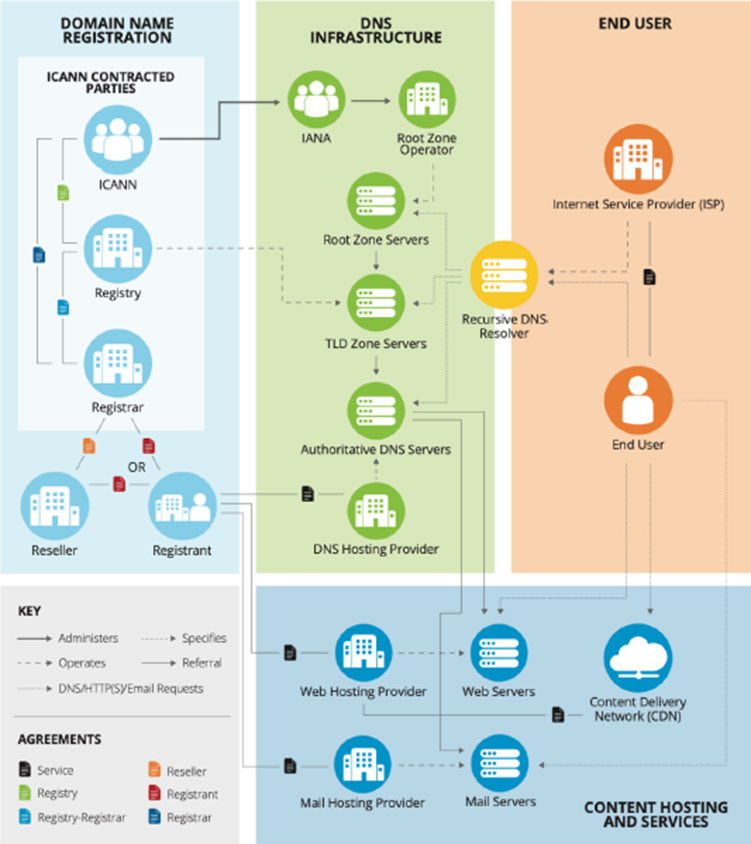
\includegraphics[width=1.0\linewidth]{background/DNSECO.png}
    \caption{DNS Ecosystem Contractually Related to ICANN (image
courtesy of Verisign and originally published in SSAC 115)}
    \label{fig:fig14}
\end{figure}
\clearpage

\section{Technological Advancements}

The mitigation of DNS abuse is increasingly influenced by the integration of artificial intelligence (AI) and machine learning technologies \cite{goethals2021enabling}. At the helm of this evolution are innovative tools like the iQ Domain Risk Score, which employs machine learning and string analytics to proactively detect potential domain abuses now of registration \cite{dnsabuseAI2023}. This tool aims to act as a mitigation measure by analysing domains against criteria indicative of malicious intent, thereby attempting to stop abuse before it even starts. Additionally, the field is witnessing a transformative shift in analysing abuse report evidence through the adoption of Large Language Models (LLMs), such as generative pre-trained transformers (GPTs). These models are highly adept at parsing and understanding complex data patterns that might be missed by human investigators, enhancing the efficiency and automation of DNS abuse mitigation efforts, and forming a more dynamic defence against cyber threats. However, this progress also highlights an emerging challenge: the potential for malicious entities to exploit AI technologies themselves \cite{halvorsenAI2023}.  Consequently, the intersection of AI and machine learning with DNS abuse mitigation not only heralds significant advancements in cybersecurity strategies but also emphasizes the need for vigilance to prevent these technologies from being used for harmful purposes. This pivotal moment in the fight against DNS abuse underscores the need for ongoing innovation and adaptation to effectively secure digital ecosystems.

\subsection{Role of AI \& Machine Learning}

The introduction of AI and machine learning technologies into DNS abuse mitigation marks the beginning of an innovative era focused on the proactive detection and neutralisation of cyber threats \cite{tariq2023critical}.  This approach facilitates the rapid analysis of large datasets to uncover patterns indicative of malicious intent in DNS queries. For example, machine learning techniques have been highly effective in analysing DNS queries to classify domain names, significantly improving the detection of domains linked to malware \cite{LiMaliciousDomainDetection2020}. Furthermore, the application of neural network models, such as the Extreme Learning Machine (ELM), has achieved accuracy rates above 95\% in identifying malicious domains, demonstrating the transformative and predictive power of AI in combating cyber threats \cite{ZouDNSGraphMining2015}. Additionally, the technique of DNS graph mining has illuminated AI's potential within cybersecurity frameworks, with methodologies like belief propagation algorithms achieving high precision in identifying infected hosts and malicious domains. These examples underscore the vital role of AI and machine learning in bolstering DNS abuse, paving new avenues for early detection and swift mitigation of potential abuses. However, the complexity of AI models and the demand for transparency in their decision-making processes present ongoing challenges. Integrating AI into DNS abuse mitigation strategies improves security measures, but also requires careful attention to ethical considerations and the establishment of governance frameworks \cite{AntonakakisMalwareDomainsUpperDNS2011}. AI and machine learning can help improve DNS abuse mitigation, but experts need to fix problems by being clear. People are worried about understanding why complex systems make choices because of the "black-box" part. It is important to understand how AI models make certain decisions. This helps to build trust and ensures that people are responsible for them. There are difficulties in making things clear, such as needing to write down what data was used for training, telling others about the things that affect choices, and explaining how models change to face new risks. It is still hard to find the right balance between the complexity needed for good threat detection and the openness needed for blame.

In summary, leveraging AI and machine learning for DNS abuse mitigation signifies a transformative shift in cybersecurity practices. The strategic application of these technologies substantially strengthens the DNS system's defence against a wide array of cyber threats, marking a significant advancement in the ongoing battle against digital abuse.

\section{Case Studies and Real-World Applications}

In recent years, technology has become so widespread that we have witnessed an unmatched number and complexity of cyber threats. A significant vulnerability that can be exploited is the DNS domain name system, a critical part of the internet infrastructure that translates human-readable names into IP addresses \cite{kumari2021sac115}. 

\begin{enumerate} 
\item\textbf{ Case Study 1: XYZ Corporation }

In this case, the study completely analyses one specific company, XYZ Corporation, as an example of DNS abuse in the real-world environment and analyze all details through figures, graphs, and charts. This abuse of DNS took place as a prolonged campaign against XYZ Corporation, a multinational technology conglomerate \cite{mohammed2021network}. Attackers used weaknesses in the company's DNS infrastructure to perform various malicious activities, including domain hijacking, DNS tunneling, and DDoS attacks. A timeline graph was also prepared to see the scale of abuse and how attacks progressed with each event that occurred in the organisation, as shown in Figure \ref{fig:figureOne}.

\captionsetup{font= footnotesize}
\begin{figure}[H]
\centering
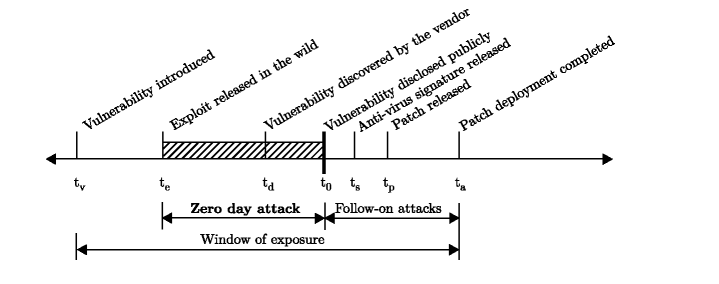
\includegraphics[width=0.9\textwidth]{background/XYZ1.png}
\caption{Timeline of DNS Abuse Attacks on XYZ Corporation}
\label{fig:figureOne}
\end{figure}

The relationship between this correlation raises questions about the attackers' understanding of the inner workings of the firm, as well as insider threats. A closer analysis of the DNS abuse types employed by such offenders revealed that domain hijacking was common \cite{bayer2022study}. Figure \ref{fig:figureTwo} shows how various DNS abuse techniques were used in the case of XYZ Corporation, and domain hijacking was significantly higher than all other combined methods.
\captionsetup{font= footnotesize}
\begin{figure}[H]
\centering
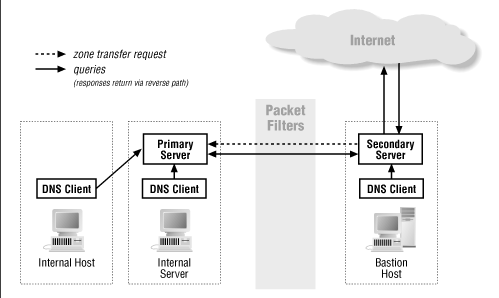
\includegraphics[width=0.8\textwidth]{background/XYZ2.png}
\caption{Distribution of DNS Abuse Techniques Against XYZ Corporation}
\label{fig:figureTwo}
\end{figure}

There is a domain hijacking technique where attackers may effectively take control over a company without authorisation; domain hijacking is one of the major threats to the organisations that are affected. The figure shows that strong security is key to preventing unauthorised access to domain registration accounts; favouring multi-factor authentication is the way to keep these attacks away \cite{paz2020cyber}. This case study sheds light on the subtleties of DNS abuse as it targeted XYZ Corporation, showing the importance of understanding and dealing with an unpredictable cyber threat environment. Figures, graphs, and graphs serve to illustrate safeguard attack procedures and give credence to the notion that an all-encompassing cybersecurity strategy is integral to mitigating DNS abuse in the digital landscape of the networked world of our day.


\item\textbf{ Case Study 2: OilRig DNS Tunneling Attack }

The case of OilRig reflects the use of custom DNS Tunneling protocols for command and control (C2) operations, thus making it dual use in nature, both in normal operation and on a fallback communication channel \cite{paloaltonetworks2021dnsattacks}.The xHunt campaign \cite{unit42_xhunt_2021} followed a similar trend of including Snugy backdoor implants in Middle Eastern government organization targets and keeping track of them using DNS tunneling for communication with its C2.  Which are examples that underscore the strategic use by adversaries of DNS tunneling techniques for stealthiness and resilience within the context of their operations  \cite{unit42_2021}.

\captionsetup{font= footnotesize}
\begin{figure}[H]
    \centering
    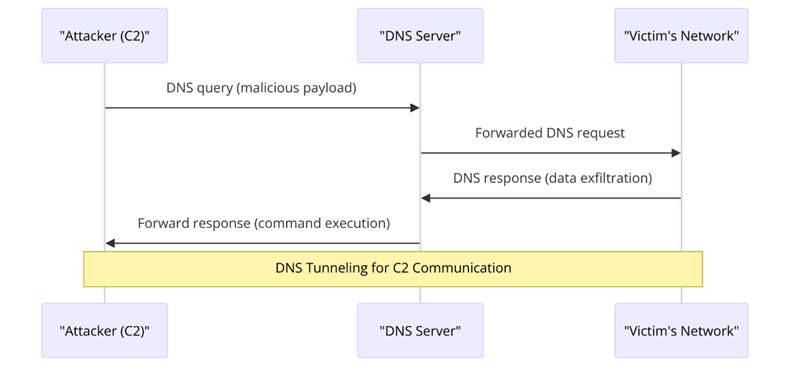
\includegraphics[width=0.8\linewidth]{background/DNSTuu.png}
    \caption{DNS tunneling communication between the attacker's command and control (C2) infrastructure and the victim's network}
    \label{fig:figTen}
\end{figure}



\item\textbf{ Case Study 3: SUNBURST Use of DGAs}

SUNBURST backdoor associated with the breach of the SolarWinds supply chain represents a case in which the use of DGAs is critical, if not only, to conceal communications and system details \cite{paloaltonetworks2021dnsattacks}. The SUNBURST backdoor applies the deep use of DNS manipulation for evasion purposes and subsequent attack stages by encoding basic system identifiers and the usage of DGAs for C2 check-ins \cite{unit42_solarstorm_2021}.

\captionsetup{font= footnotesize}
\begin{figure}[H] 
    \centering
    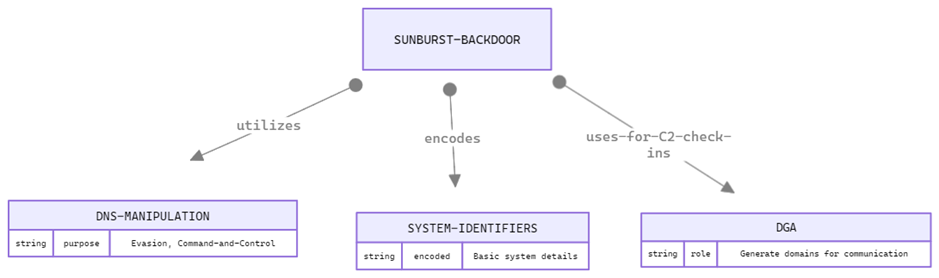
\includegraphics[width=0.8\linewidth]{background/SUNDNS.png}
    \caption{SUNBURST backdoor's utilization of DGAs and its associated components}
    \label{fig:figEleven}
\end{figure}

\item\textbf{ Case Study 4: Fast Flux Techniques}
The presence of several C2 domains related to the Smoke Loader malware family using Fast Flux techniques only further underscores the difficulties associated with the tracking and eradication of DNS-enabled threats. \cite{paloaltonetworks2021dnsattacks}.The major takeaway in the rapid rotation of IP addresses of this method points to the dynamism of strategies used in communications by malware, thus improving the means of defence by cybersecurity \cite{unit42_fastflux_2021}.

\captionsetup{font= footnotesize}
\begin{figure}[H]
    \centering
    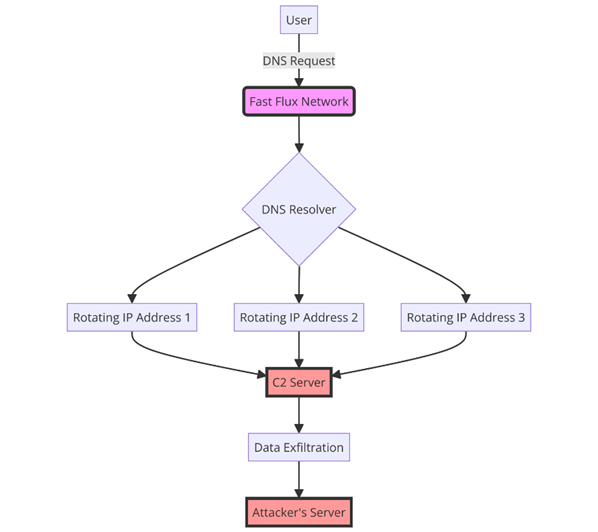
\includegraphics[width=0.8\linewidth]{background/FastFluDNS.png}
    \caption{The usage of Fast Flux techniques by the Smoke Loader malware family for dynamic C2 domain communications}
    \label{fig:figTweleve}
\end{figure}


\item\textbf{Case Study 5:  Malicious Newly Registered Domains (NRDs)}

The malicious NRDs opportunistically crafted in the milieu of the pandemic expose how threat actors leverage current events for engineering targeted attacks. \cite{paloaltonetworks2021dnsattacks} From domains that mirror COVID-19 information resources to those faking government relief programmes, the evolution of such attacks reflects a calculated approach to exploiting public interest and vulnerabilities  \cite{unit42_covid19_phishing_2021} .

\captionsetup{font= footnotesize}
\begin{figure}[H]
    \centering
    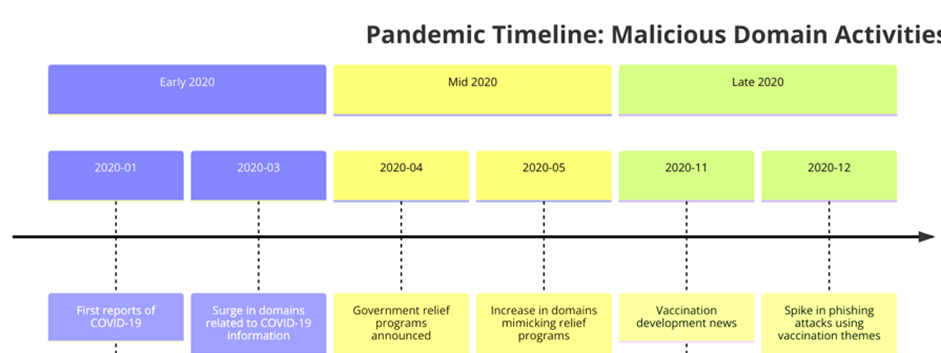
\includegraphics[width=0.8\linewidth]{background/PandemicTime.png}
    \caption{The usage of Fast Flux techniques by the Smoke Loader malware family for dynamic C2 domain communications.}
    \label{fig:figThirteen}
\end{figure}

\end{enumerate}

In the coronavirus pandemic, too, phishing attacks changed to initially targeting PPE and testing kits, then turning to government stimulus programs, and subsequently enlisting vaccine distribution. Several of them, in fact, employed sophisticated tools like MFA pretending as US Federal Trade Commission and brands such as Pfizer and BioNTech, to steal credentials. where it emphasized that there was a 530\% surge in vaccine-related phishing attempts and a 189\% hike in attacks on pharmacies and hospitals from December last year to February this year. Advice was given for individuals and organisations that include being cautious in email and website dealings, stepping up security awareness training, as well as adopting multi-factor authentication.

Since January 2020, a total of 69,950 COVID-19 related phishing URLs have been received, of which 33,447 are specifically dedicated to COVID-19. The data has been normalised in such a way that the peak of each topic is at 100\%. The results showed much steadier phishing when it came to topics such as pharmaceuticals and virtual meeting platforms (e.g., Zoom) with vaccines and testing showing sharper rises and falls in the attention of scammers.

\captionsetup{font= footnotesize}
\begin{figure}[H]
    \centering
    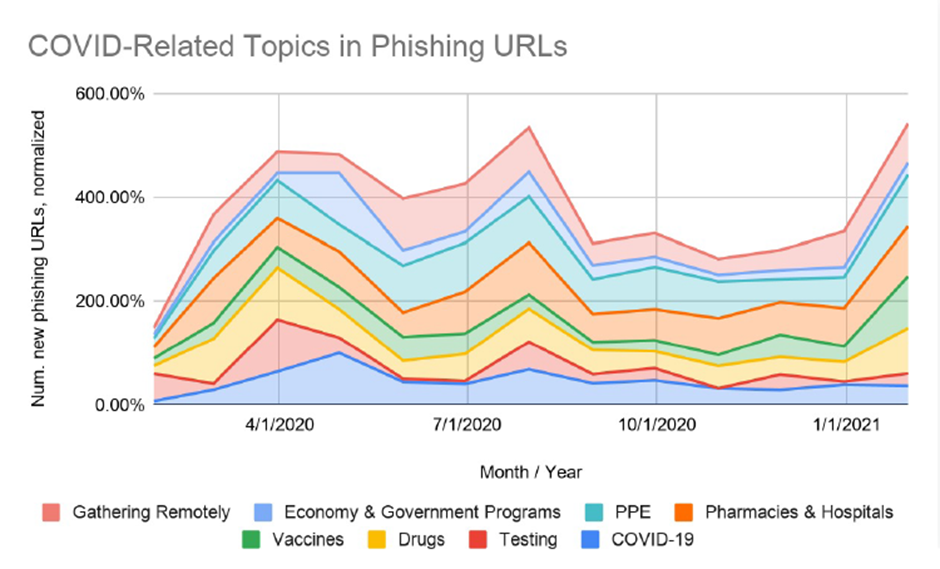
\includegraphics[width=0.8\linewidth]{background/CovidPhising.png}
    \caption{Development trends in the majority of COVID-19-related phishing content hosting sites during the period from January 2020 to February 2021.}
    \label{fig:figFourteen}
\end{figure}

It is evident to state that a major chunk of COVID-19-themed phishing pages targeted leading brands for phishing business credentials, such as Microsoft login, Webmail, and Outlook login. For example, about 23\% of these phishing URLs were posed as Microsoft login pages. This threat has particularly highlighted the shift towards remote work in the pandemic and, hence, magnified the relevancy of these attacks as one of the foremost methods to be undertaken by bad actors .


\captionsetup{font= footnotesize}
\begin{figure}[H]
    \centering
    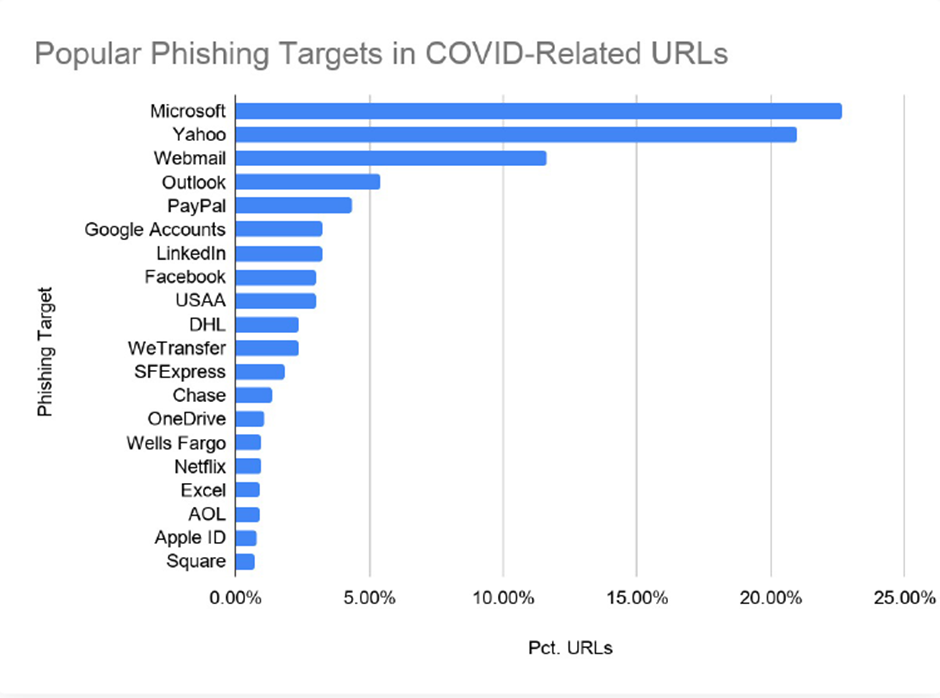
\includegraphics[width=0.8\linewidth]{background/TOPCOVIDURLS.png}
    \caption{Top spoofed websites in COVID-themed phishing attacks (global), where the percentage in each column is the percentage of phishing volume per site and category. }
    \label{fig:figFiveteen}
\end{figure}

This thus clearly indicates a situation whereby the attackers set up websites frequently for COVID-19 themed phishing attacks. Many of these phishing pages are found on sites created less than 32 days, meaning these sites are launched with specific purposes in view of these imminent attacks. The strategy allows attackers to customise their messages and URLs to the current pandemic trends, indicating the dynamism behind such cyber threats.

\captionsetup{font= footnotesize}
\begin{figure}[H]
    \centering
    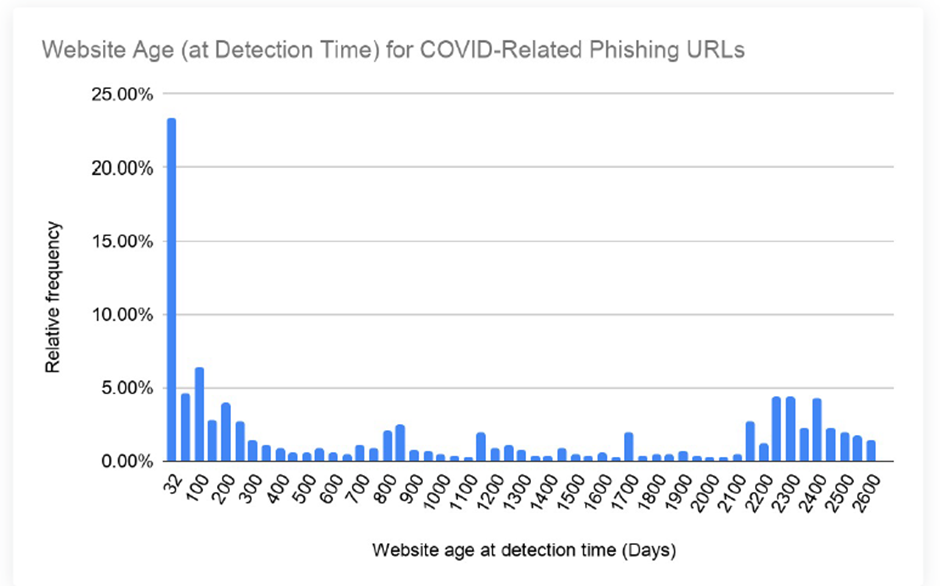
\includegraphics[width=0.8\linewidth]{background/AgeCovid.png}
    \caption{Statistic of lifespan distribution of COVID-19-related phishing content hosting sites when the sites are reported .}
    \label{fig:figSixteen}
\end{figure}


\section{Challenges \& Future Directions}

Mitigating DNS abuse demands an immediate stop to the escalation and rapid evolution of cyber threats, underscoring the critical need for swift global cooperation and the implementation of advanced technology. The key challenge is to achieve a fine balance between reducing false positives and accurately identifying genuine threats, while simultaneously advancing beyond the limitations of outdated technologies \cite{pour2023comprehensive}. The future of this domain largely depends on researchers' ability to enhance technological solutions, particularly focusing on the improvement of AI algorithms for deeper analysis of DNS traffic patterns. This opens a promising pathway for the creation and application of locally developed tools, providing innovative strategies to strengthen DNS defences. The ability to navigate the complex landscape of DNS abuse will require stakeholders to be agile in responding to emerging threats and developing novel solutions. The collective push towards the evolution of technology and methodologies will play a pivotal role in shaping effective DNS abuse management strategies in the years ahead.


\subsection{Identification of Current Challenges}

Mitigating DNS abuse involves developing strategies that should be not only proactive but kept constantly up to date to handle the changing environment of cyber threats. The fluid nature of these threats means updating current protocols as well as developing new defence methods. With cybercriminals constantly revising their methods of capitalising on the vulnerability of DNS, it has become imperative for the cybersecurity industry to continuously update its defence mechanisms \cite{bhattacharya2023dns}. Being a global phenomenon, the internet, and hence DNS abuse being transnational in character, there is no other alternative than international cooperation. The effectiveness of the DNS abuse management would be based on collaborative work across national borders, where experts in different geographical areas come together to share their knowledge and resources \cite{altulaihan2022cybersecurity}. Legal and regulatory framework varies in the several jurisdictions, thereby making it difficult to reach a consensus on the regulations, standards, and enforcement action. Another big challenge is that, to mitigate DNS abuse, the requirement for driving down both false positives and negatives is necessary. Balance must be established in such a way that rather strict measures may reduce user experience, while, at the same time, being liberal might bring less detection of malicious activities . The cybersecurity community must continue to advance its detection and response capabilities, due to the increasing levels of sophistication used by DNS abusers. This will keep the security and integrity of the DNS system in good shape, hence protecting this vital part of internet infrastructure.

\subsection{Discussion on Future Research Directions and Technologies}

When planning to mitigate the DNS abuse in the future, discussing new research ideas and upcoming technology is important. The constantly changing state of Internet threats requires us to continually create new things. This is so people can stay one step ahead of the bad people. Future work on DNS abuse needs to start by building better tools. These can help to address how bad guys on the Internet keep changing their tricks \cite{bovenzi2023blockchain}. This means that we need to look at more complex AI and machine learning tools that can understand the details of web traffic, which will make the results more accurate and stop wrong signals from being sent. Moreover, there is a rising need to use blockchain tech to make domain registration safer and stop any bad or harmful changes, as it provides decentralised domain name resolution unlike traditional DNS systems, which rely on a central authority to resolve domain names in which DNS operates on a network of distributed nodes in which each node has a copy of the entire ledger, so it can independently verify and resolve domain name requests, which not only makes the system more resilient to attacks, but also prevents censorship and control by a single entity. \cite{FinanceStrategists2023BlockchainDNS}.  People should have easy methods to report DNS abuse. This will make sure everyone knows about dangers \cite{gu2021iot}. Working together in the world is very important because computer dangers go beyond borders. 


\section{Summary of Findings}

The study on DNS abuse looked at current ways, checked new trends, talked about tech advancements, and explored real examples in life. The search for ways in the plans to mitigate DNS abuse showed the value of clear communication and honesty in building trust with the community. People are finding new ways to abuse the DNS system. Researchers have to keep making new things, so they don't get caught by changing dangers. Improvements in technology, especially with artificial intelligence and learning machines, showed how automation can make it easier to spot dangers. But it also made things harder to understand, and this needs careful attention. Examples from real life showed what did and did not work in making DNS abuse clearer. These provided essential advice for the business. Issues were found with making things clear and stopping wrong actions. This shows how important it is to continue learning and working with others. In the future, discussing issues and future plans will show the need for creative studies, help from other nations, and common ways to share information. 

\section{Conclusion}

DNS abuse continues to be a big issue. Present plans, while sometimes useful, require constant adjustment and getting better. It's key to have solutions for fixing issues available. This helps to build trust and work well with those involved. Abusing DNS in new ways brings new issues that require clever solutions. AI and machine learning can help find things, but we need to show how they work better so that people can keep bad people under control. Learning from real-life situations teaches us a lot about good and bad ways of being open. This helps us create the best methods for our business. There are still issues with showing and stopping DNS abuse while trying to find new ways to mitigate this DNS abuse. People need to continue learning and working as a team. People should focus on better technology, joining forces with other nations, and using common methods of sharing information in the future. As the internet changes, we must stay active and work together to stay ahead of bad people who want to hurt us. 





















\chapter{Research Methodology}



A structured questionnaire was sent by email to various stakeholders in the DNS ecosystem. This method was chosen because of its convenience, compliance with participants' busy schedules, and permission for detailed responses at the respondents' will. The approach provided a means of collecting a wide range of observations on DNS abuse in terms of definition, the most prevalent types, mitigation challenges, and the theme of transparency. 



\section{Questionnaire Design and Distribution} 

The questionnaire had to take into account some of the issues in a multidimensional approach, giving great emphasis, but not limited, to address the nature of DNS abuse mitigation transparency.

The questions were specifically designed to extract in-depth information about:


 \begin{enumerate}
 \item The definition of DNS abuse. 
 
  \item The types of DNS abuse stakeholders are most frequently encountered, with the aim of identifying patterns and specific concerns within the ecosystem.
  
  \item The challenges and limitations faced in mitigating DNS abuse, seeking to understand the barriers to effective action.
  
  \item The mitigation strategies used, gathering information on the practical steps taken and their perceived effectiveness.
  
  \item The practice of publishing reports or data as a form of transparency, exploring the current state of openness in the field.
  
  \item The role of transparency in aiding or impeding DNS abuse mitigation efforts, probing the potential impacts of increased visibility.
  
  \item  The effects of transparency on the relationships between various DNS stakeholders, considering the broader implications for cooperation and trust.
\end{enumerate}


\section{Stakeholder Responses} 

The insights from the completed questionnaire of the different stakeholders reflect several key themes and insights into understanding DNS abuse, as well as the mitigation of this abuse which provide a full view of current practices and potential areas for improvement with respect to the DNS ecosystem. The key themes and insights include:



\begin{itemize}
  \item \textbf{Varied Definitions of DNS Abuse:} Although stakeholders largely accepted the definition that had been adopted by the ICANN Contract Parties, they also noted its shortcomings, especially in being too categorical and thus may leave out evolving types of abuse. It was considered that a more flexible way forward would be a robust framework to define the abuses to be mitigated at the domain name level.
  
  \item \textbf{Common Types of DNS Abuse:} They pointed out that phishing was the most common attack type, followed by malware, botnets, and spam. It was also pointed out that one of the most common problems was related to the challenge related to proving the number of spam-related domains.
  
  \item \textbf{Challenges in Mitigation:} Perhaps the most significant was the economic structure of the domain registration industry and its ability to mitigate malicious registrations without fundamentally altering it. Stakeholders clearly state that a significant difference between large registrars, generally considered good actors on the Internet, and smaller registrars with a higher level of DNS abuse underscores the different aspects of this problem within different industry segments.
  
  \item \textbf{Mitigation Strategies:} Responses include different strategies, from blocking orders from some regions to the use of software to monitor abusive activities. Recommendations were made in the area of education and outreach projects, such as NetBeacon and Compass, to report abuse and information on DNS abuse.
  
  \item \textbf{Role of Transparency:} Opinion on the transparency process was kind of mixed, since part of the respondents consider this positively because it is a tool that provides evidence to the industry in their fight against abuse and part of them consider negatively the way sensitive mitigation ways could be revealed. The consequence of transparency was elaborated on the development of relationships between all stakeholders, and there is, in general, a common understanding that transparency would increase understanding and teamwork through better communication on set measures against abuse.
  
\end{itemize}

Thus, the responses of stakeholders were quite valuable in providing a snapshot of practical challenges and possible mitigation strategies for DNS abuse. Consequently, it was a very valuable presentation of a real-world view of the need for the world to have adaptive definitions and comprehensive mitigation strategies, along with transparency in the ecosystem. This further extrapolates the theoretical knowledge with the help of the experiences of people involved on an active basis in the mitigation of DNS abuse.

\section{Types of DNS Abuse Encountered} 

The stakeholder responses described the most common form of DNS abuse assumed within their area of interest. From these, views emerge for a variety of threats, where each of them brings unique challenges that favour specific mitigation measures.

\begin{enumerate}
    \item Phishing: Stakeholders identified it as the most prevalent form of DNS abuse and the most visible. In fact, the total number of phishing incidents observed through tools such as NetBeacon and tracked by Compass is a stark and singular metric of just how big and urgent the problem has become in the wider DNS domain.
    \item Malware and Botnets: These also included malware and botnets, i.e. multifaceted DNS abuses. Such abuses not only compromise the integrity of systems, but also present a security hazard to users and infrastructures, in general.
    \item Spam: It is now recognised as widespread, and stakeholders have pointed out the challenges of quantifying and appropriately addressing the relevant spam-related domains. Therefore, it makes spam elusive for existing mitigation efforts that raise the bar in the pursuit of next-generation detection and response mechanisms.
    \item Compromised CMS: Common encounters with the content management system (CMS) compromised. Consequently, attacks remain possible where some other existing vulnerabilities on web platforms are concerned. This kind of abuse is the reason why strong web security control practices should be in place and why platform operators must be alert.
    \item "Water Torture" Attacks: Known as random subdomain attacks, they are even more technical and sophisticated ones. Such attacks not only compromise the regular functioning of DNS but also take some of the most sophisticated countermeasures to mitigate its impact on the affected parties.
\end{enumerate}

The continued variation in DNS abuse experienced by stakeholders indicates that community efforts in terms of collaborations, innovations, and education will build on the experiences derived from stakeholders and inform the most relevant foundation on which effective strategies and policies will be developed to mitigate DNS abuse effectively.

\section{Challenges in Mitigation and Mitigation Strategies} 

The responses of the stakeholders demonstrated details of the multifaceted challenges in mitigating DNS abuse, coupled with the various strategies used to address these issues.
\begin{enumerate}
    \item Economic and Technical Hurdles: A clear barrier related to the economic nature of the DNS industry was identified, which is characterised by low margins and high volumes, leaving little resources to help mitigate DNS abuse on a large scale. The responsible registrars stressed that 80\% of the malicious domain name registrations were related to several large and reputable registrars and some small registrars, which is an example of how, from an economic point of view, the cost of security is not proportional to the amount of dangerous information that is being exploited. This points to a clear economic barrier in the DNS ecosystem and calls for new ways of efficient and economical mitigation.
    \item Regulatory Gaps: The regulatory environment was mentioned as a challenge. Included poor, weak, or lack of policies and enforcement mechanisms that did not allow us to combat DNS abuse properly. Therefore, all respondents also emphasised the need for more clear regulations and standards that could better guide industry attempts to mitigate abuse.
    \item Mitigation Strategies: They have focused on components of education, collaboration, and outreach to create knowledge and a social response. Software tools to support these efforts, abuse reporting intermediaries and measurement projects that measure the Internet, are crucial in finding, reporting, and understanding abuse cases. These tools are also designed to help report and mitigate risk, but can collect critical data with a policy and the character of a regulatory response.
    
    
\end{enumerate}


\section{Transparency in DNS Abuse Mitigation} 

The responses of stakeholders underscore the subtle perspective on transparency within the DNS abuse mitigation framework, highlighting both its potential benefits and challenges.

\begin{enumerate}
    \item Benefits of transparency: Transparency is increasingly recognised as a method for sector participants to show a firm-wide commitment to combating DNS abuse. By allowing mitigation efforts to be driven down the stack and done more rapidly and often overtly, the action becomes associated with a culture of accountability and responsibility. However, when it comes to issuing data on the prevalence of abuse and the effects of mitigation measures, transparency can strengthen confidence among users, regulators, and sector participants. Furthermore, it is acknowledged as a contributing element to a comprehensive understanding of and collaboration among the various actors in the DNS landscape. Operators, registrars, registries, and regulators may have a better understanding of the difficulties and achievements of many other performers in the section if they exchange data on abusive activities and mitigation measures.

    \item Challenges and Concerns: Stakeholders raised several concerns about the degree and manner of transparency. One fear is that some sensitive mitigation strategies are being disclosed and could serve as a means for the bad guys to find ways to find out about abuse and its mitigation. Many within the industry find here a fine balance between useful information on the one hand and, at the same time, protecting operational integrity on the other. Additionally, there is apprehension that increased transparency could lead to regulatory or legal consequences, especially if disclosures are mandated in a manner that does not consider the practical aspects of abuse mitigation. Stakeholders also pointed out such operational challenges as the ability to complete transparency reporting, given the current reliance on less formal mechanisms to report abuse and monitoring mitigation.
    
    \item Strategic Approach to Transparency: The stakeholders are for the vision that a strategic approach to transparency in support of the goals and aims for mitigation of DNS abuse should, in no way, be undermined from being effective. This would include targeted transparency, with the point being more aggregated data and trends than detailed disclosure of specific mitigation actions or techniques. But this environment should be nourished where sharing information does not result in punitive consequences, but, on the other side, supports collaborative improvement, which is considered essential. The value of transparency for the mitigation of DNS abuse is considered of high value, but stakeholders advise to be careful with each step in what, how and to whom it will be disclosed. This shall be a balanced approach that increases the collective ability to address DNS abuse, rather than safeguarding methods used. In short, it is of the utmost importance for the continual evolution of transparency practices in the industry.


\end{enumerate}

\section{Impact on Relationships within the DNS Ecosystem} 

 Stakeholders pointed to a clearer potential impact on meaningful relationship building within their particular DNS ecosystems: greater transparency and mitigation. Better transparency is seen by creating a better understanding among different parties, for instance, among registries, registrars, and regulators about challenges and works against abuse, hence their collaboration and trust that improves combined efforts against abuse. However, this provision raises concerns that such transparency could get to the point of obstructing informal cooperation in general or actually reveal sensitive techniques from an operational standpoint detrimental to entities working together. Balance is a key element to ensure that these issues are addressed and that partners work harmoniously with each other within the DNS community.

\section{Analysis and Data } 

The following is a summary of the emailed responses of the stakeholders in relation to DNS abuse mitigation. In relation to those themes, the following record the main important points.


{
\begin{table}[H]
\centering
\footnotesize 
\begin{tabular}{|p{3cm}|p{9cm}|}
\hline
\cellcolor{gray!50}\textbf{Definition Supported} & 
\cellcolor{gray!50}\textbf{Comments and Suggestions} \\
\hline
\mbox {ICANN Contracted} Parties' Definition & Endorses the ICANN definition for its clarity and actionability. However, it suggests that it may be too narrow and advocates a more flexible framework to encompass evolving threats. Points to a self-authored sophisticated way of defining harms at the domain name layer, promoting adaptability. \\
\hline
\mbox {Critique of} ICANNwiki Definition & Finds the ICANNwiki reference lacking, preferring the SSAC 115 report definition for its broader applicability and recent adoption in RAA amendments. \\
\hline
Mixed Views & \mbox {While there is alignment with the existing categorical} \mbox {definitions for practical reasons, there is a shared belief in the} necessity for definitions that evolve with emerging DNS \mbox {threats. The discussion indicates a desire for a balance} between categorical clarity and adaptability to new forms of abuse. \\
\hline
\end{tabular}
\caption{Varied Definitions and Understandings of DNS Abuse}
\label{table:dns_abuse_definitions}
\end{table}

}

{
\begin{table}[H]
\centering
\footnotesize 
\begin{tabular}{|l|l|p{5cm}|}
\hline
\cellcolor{gray!50}\textbf{Type of DNS Abuse} & 
\cellcolor{gray!50}\textbf{Frequency Mentioned} & 
\cellcolor{gray!50}\textbf{Stakeholder Comments} \\
\hline
Phishing & Most Common & \mbox {Identified as the primary concern} \mbox {across responses, significant} impact observed. \\
\hline
Compromised CMS and Confusable Domains & Frequently Mentioned & \mbox {Highlighted as a prevalent issue} \mbox {alongside phishing and other} platform abuses. \\
\hline

\end{tabular}
\caption{Types of DNS Abuse Encountered}
\label{table:types_of_dns_abuse}
\end{table}
}

{

\begin{table}[H]
\centering
\footnotesize 
\begin{tabular}{|l|p{4cm}|p{4cm}|}
\hline
\cellcolor{gray!50}\textbf{Challenge Type} & 
\cellcolor{gray!50}\textbf{Stakeholder Insights} & 
\cellcolor{gray!50}\textbf{Suggested Solutions} \\
\hline
Economic & \mbox {High volume, low margin} \mbox {business model impedes} anti-abuse efforts. & \mbox {Calls for industry-wide} collaboration and support. \\
\hline
Regulatory Gaps & \mbox {Lack of clear regulations} \mbox {complicates mitigation} efforts. & Advocates for establishing and following industry-wide best practices. \\
\hline
\end{tabular}
\caption{Challenges in Mitigating DNS Abuse}
\label{table:challenges_in_mitigation}
\end{table}


}

{

\begin{table}[H]
\centering
\footnotesize 
\begin{tabular}{|l|p{4cm}|p{4cm}|}
\hline
\cellcolor{gray!50}\textbf{Strategy} & 
\cellcolor{gray!50}\textbf{Description} & 
\cellcolor{gray!50}\textbf{Stakeholder Feedback} \\
\hline
Blocking Orders & \mbox {From certain regions to} mitigate abuse. & \mbox {Implemented alongside} \mbox {other criteria to make} \mbox {services less appealing to} abusers. \\
\hline
Education \& Collaboration & \mbox { Outreach to improve} awareness and cooperation. & \mbox {Viewed as essential, with} \mbox {a need for more systematic} implementation. \\
\hline
\end{tabular}
\caption{Mitigation Strategies Employed}
\label{table:mitigation_strategies}
\end{table}

}

{
\begin{table}[H]
\centering
\footnotesize 
\begin{tabular}{|l|p{4cm}|p{4cm}|}
\hline
\cellcolor{gray!50}\textbf{Aspect of Transparency} & 
\cellcolor{gray!50}\textbf{Benefits} 
& \cellcolor{gray!50}\textbf{Concerns} \\
\hline
Reporting Abuse Metrics & \mbox {Enhances trust and} \mbox {accountability in the} ecosystem. & Risk of exposing sensitive mitigation techniques if not managed carefully. \\
\hline
\end{tabular}
\caption{Transparency in DNS Abuse Mitigation}
\label{table:transparency_in_mitigation}
\end{table}


}

When analysing the data from the stakeholder responses, a thorough examination of DNS abuse was carried out. The stakeholders provided valuable information on the definitions of DNS abuse. The commonly mentioned type was phishing due to its spectrum in all aspects, compromised CMS, and confusables were also identified by everyone as prevalent. The most challenging aspects of mitigation included economic factors that influence achievable levels of DNS abuse in the branch and regulatory gaps because the market structure changes the evaluation of mitigation abuse measures and the lack of set regulations blurs perceptions. The mitigation strategies and plans implemented are based on targeted blocking and collaborative education; their efficiency is reduced by the industry's focus on performance and the paths of different entities. Transparency is described as a double-sided weapon; although it has accountability and trust-building potential, it can harm the industry when people use their malicious understandings. Stakeholder experiences and actions contribute to the understanding of DNS abuse, maximising the need for a multidimensional approach based on adaptation, cooperation, and the equivalence of transparency.


\chapter{Draft}

\section{Confusable Domains}
\subsection{Identification and Examples of Targeted Domains}

The choice of such domains to target and outsource depends on many factors, each with its implications on the business strategy, marketing, and observance by law. The selection of these domains hence matters a lot in creating potential conflict especially those related to existing trademarks. Understanding these selection criteria is very important to try to negotiate the hurdles of the digital market and to protect rights through intellectual property. 

To navigate these complexities effectively, it is essential to consider several key factors. 

\begin{itemize}
  \item \textbf{Commercial Appeal:} High commercial appeal domains are lucrative targets due to the extremely high possibility of attracting a large traffic flow, with potential revenue generation. Such names are easy to remember, short in length, and directly linked to products or services under some category that is searched most frequently.\cite{Li2002ConflictDomainTrademark}
  
  \item \textbf{Keyword Relevance:} Targeted domains have a certain relevance that holds the keyword itself. These domains are ranked higher in search engine outputs and attract organic traffic, making them a useful tool for businesses aiming to align with the primary keywords used by their target customers.
  
  \item \textbf{Similarity to Well-known Trademarks:} This refers to the practice of registering domains that are similar or confusingly like existing trademarks—known as cybersquatting. This can lead to confrontations with the rightful trademark holders. Trademark law aims to prevent consumer confusion and protect the goodwill associated with the trademark, particularly in disputes over domain infringement.
\end{itemize}

\subsection{Real-life examples}

\begin{itemize}
    \item \textbf{Cybersquatting :} is securing domain names that are the same as or in the likeness of trademarks or brand names, with the intent to sell them at grossly marked-up prices back to the true owner. Among the most notorious examples are several court battles based on the purchase of "nissan.com" and "nissan.net" by a person named Nissan, who owned Nissan Computer Corp many years before Nissan Motors tried to acquire it. This case highlighted tension between the protection of trademarks and individual's interests in using their names for domain name purposes as well as it underscores the challenges of domain name registration and trademark protection in the digital age where domain names closely resemble established trademarks, potentially leading to consumer confusion and dilution of trademark’s value. \cite{Rosznyai2005}
    
    \item \textbf{Typosquatting- URL hijacking :} it deals with the registration of misspelled variants of well-known domain names for the mere purpose of capturing traffic from users who tend to make mistakes in typing a URL. They could register "goggle.com" instead of "google.com" which was used to direct users to a site that bombarded their browsers with pop-ups and ads , leading to malware infections as that site was designed to capitalize on accidental misspellings or phishing  attempts that tricked users into visiting. \cite{SplunkTyposquatting}

     \item \textbf{Reverse Domain Name Hijacking  :} is the act of trademark owners trying to take a domain away from its rightful holder based on the claim of trademark rights, considering that he holds a bona fide registration over the said domain. It may otherwise be described as using legal or dispute resolution mechanisms to try to force people from their domains. \cite{Sun2006DomainTrademarkConflict}

    An RDNH was claimed in a UDRP action against "groovle.com," in which the domain was purported to be too close to Google's trademark. However, since the domain was used for another search engine, it was deemed legitimately used and not to have infringed on Google's trademark or registered in bad faith. \cite{Singh2011ReverseDomainHijacking}

    \item \textbf{Homograph attacks:} are those cases in which people have registered domains using characters that kind of look similar to those used on legitimate sites for instance, using a homographic character to make 'Google.news' appear as 'google.news'. This technique has been followed by fraudsters who are now imitating various Google domains for phishing purposes. The group said it reported similar flaws with applications such as Signal and Telegram, where homograph attacks deceived the user to visit harmful sites by using Unicode in domain names to look like famous brands, including phishing attempts on MyEtherWallet and GitHub users. \cite{Leyden2021}
\end{itemize}

\subsection{ Real-life Mitigations}

The following scenarios are examples of real-life confusable domain mitigations :

\begin{itemize}
    \item \textbf{Cloudflare's Zero Trust Services Approach :} Protection from this problem of newly created phishing websites is given by Cloudflare itself with its protection in the form of Zero Trust services, finding these websites, and blocking confusable domains. Cloudfare zero-trust rules can be enforced using Cloudfare Gateway in a way that they deny access to these illegitimate domains. In such a way, corporate networks are supposed to be secured from phishing attempts that take advantage of human trust in well-known brands. \cite{Cloudflare2023}

     \item \textbf{Swift-URL-SpoofCheck Initiative: } On this open source initiative hosted on GitHub, a domain renderer has been released for the WebURL format defined according to the algorithmic rules established by IDN spoof checking in Chromium has been released. This tool intends to provide the user with an additional form of safety from domains that look confusingly like known-good domains by integrating most but not all the rules that Chromium uses in the label verification process. It includes functionality to identify potential spoofs and visualise how what appear to be valid domains could be deceptive. \cite{KarwaSwiftURLSpoofCheck}
     
     \item \textbf{IDN Handling of Google Chrome: } Google Chrome enforces an IDN (Internationalized Domain Names) policy to determine which form the Unicode or punycode form a domain label should be displayed in. The domain label is tested whether it has mixed script, invisible characters, or visually confusable characters, and whether it is actually validly converted into Unicode. For instance, domains containing characters of different scripts, or those that are clearly identified as mixed script confusables, will be displayed in punycode, warning the users of potential deceptions. Chrome further offers comprehensive warnings to secure URLs that appear to be an imitation of already known web pages. \cite{ChromiumIDN}
     
\end{itemize}

In addition to what I mentioned above, let us look at the most popular mitigations used world-wide :

\begin{enumerate}
  \item Deployment of DNS Security Extensions (DNSSEC): DNSSEC introduces an additional security layer to the DNS query and response mechanism, helping protect against DNS spoofing attacks that often accompany confusable domain strategies. 
  \item Typo-squatting Detection Tool: Tools such as DNStwist and URLCrazy are used to offer organizations similar domain names so that they can either secure these domain names in advance or file litigation for the same.
  \item Anti-Phishing Working Group (APWG): It is a pool for stakeholders to share intelligence, trends and best practices regarding phishing and similar threats associated with confusable domains in which mitigation is carried out in collaboration action between cybersecurity entities and domain registrars, as it allows sharing of threat intelligence with respect or cancelling out the holding of malicious domains.
\end{enumerate}

\subsection{Collaboration Among Registrars, Registries, and DNS Collaborators}

This collaboration should be achieved with DNS registry, registry and collaborators. In that way, they can boost common resources and intelligence that can guide in making the internet more secure and resilient. This strictly falls within the remit of registries and registrars acting in collaboration to put in place such stringent registration policy with procedures for verification, checking against mimicking existing trademarks or even popular domain names.

In this way, the collaboration can even manifest itself via the sharing of sensitive data with regards to domain abuse threats and trends. Databases and threat intelligence platforms are shared amongst stakeholders, allowing them to anticipate and avert most such perils well before they impact netizens. This collective effort will enable the formulation of standards by which to coordinate responses to confusable domain incident reports. Mitigating confusable domains demands that registrars, registries, and DNS collaborators work in a common effort. This is due to the increasing level of threats and the shared responsibility of all the actors involved in the DNS ecosystem. \cite{Catania2022} To put this into perspective, here are some examples: 


\begin{enumerate}
  \item Recent changes in the contract from ICANN's contracted parties have imposed on registrars and registries new specifications to define DNS abuse, together with clear requirements for the actions to be taken by such parties immediately actionable evidence of abuse is received. This is a major step towards establishing more clarity about the roles that may be played by these different stakeholders in addressing the matter of DNS abuse and ensuring there is a common approach to redress. \cite{Weinstein2023}
  \item Approved new obligations of ICANN's contracted parties have been by the community itself further to mitigate DNS abuse, thereby demonstrating the will of the community to come together to address the issues of DNS abuse. \cite{ICANN2023}
  \item Efforts like NetBeacon, with the support of the DNS Abuse Institute, are being rolled out to reduce friction in reporting and mitigating DNS abuse. This service solves the current complexities and quality standards associated with the reporting of DNS abuse as it makes the work easier for the registrars, ultimately narrowing down their scope to the relevant and evidenced report as well as it underlines the need for cooperation among registrars, registries, and other DNS stakeholders. This is what is capable of saving the Internet and safeguarding at the same time the credibility and confidence of DNS. \cite{NetBeacon}
  
\end{enumerate}

\subsection{Techniques for Mitigating Confusable Domains}

Mitigating confusable domains requires sophisticated techniques tailored to address the unique challenges presented by both non-Internationalized Domain Names (non-IDNs) and Internationalized Domain Names (IDNs). This differentiation is crucial due to the distinct nature of threats they pose and the technical feasibility of the mitigation strategies applicable to each. Below is a detailed examination of mitigation techniques, along with discussions on the operational feasibility and potential collaboration frameworks involved.

Non-IDNs Mitigation Techniques : For non-IDNs, strategies focus on identifying and preventing domain squatting and typo-squatting, where attackers register domains that are typographical errors or close variants of legitimate domains to deceive users.

\begin{enumerate}
  \item Registry-Level Measures: Domain registries can implement checks to prevent the registration of domains that are too like existing trademarks or brand names, using algorithms to detect variations and misspellings closely resembling protected names. \cite{WTR2020} 
  \item Trademark Protection Programs: Services like the Trademark Clearinghouse (TMCH) offer mechanisms for trademark holders to protect their rights by receiving notifications when someone attempts to register a domain matching their trademark. \cite{ICANNTMCH}
  \item Automated Monitoring and Reporting: Automated systems can continuously monitor domain registrations for names that closely resemble known trademarks or brand names, enabling rapid detection and legal action against infringers. \cite{TMCH2023}
\end{enumerate}

IDNs Mitigation Techniques : The challenge with IDNs lies in the potential for homograph attacks, where attackers use characters from different scripts that appear visually like characters in the Latin script to create deceptive domains.

\begin{enumerate}
  \item Punycode Awareness and Monitoring: Web browsers and security tools convert IDNs to punycode, a representation that encodes the Unicode characters into ASCII. Awareness of punycode and monitoring for suspicious registrations can help identify potential homograph domains. \cite{SOCRadar2023}
  \item Browser-Level Defenses: Modern web browsers have implemented defenses against IDN homograph attacks by displaying the punycode version of the domain or alerting users when a domain name contains characters from multiple scripts. \cite{Malwarebytes2017}
  \item Collaborative Blacklisting and Sharing of Threat Intelligence: Organizations can collaborate to share intelligence about known malicious IDNs, contributing to comprehensive blacklists that can be used by registrars, DNS providers, and end-users to block access to malicious sites. \cite{CyberThreatAlliance2023}
  
\end{enumerate}

\subsection{Technical and Operational Feasibility}
The technical feasibility of these techniques varies. Registry-level measures and trademark protection programs are highly effective but require cooperation and standardization across different legal jurisdictions. Automated monitoring is technically feasible and can be implemented at scale but requires resources for continuous operation and legal follow-up. Browser-level defences are among the most directly impactful, protecting users at the point of access, yet they depend on browser vendors' willingness to implement and maintain these features as well as collaboration frameworks play a crucial role in mitigating confusable domains. Initiatives like the Trademark Clearinghouse (TMCH) facilitate cooperation between trademark holders and domain registries. Meanwhile, organizations such as the Anti-Phishing Working Group (APWG) and the Internet Corporation for Assigned Names and Numbers (ICANN) work towards broader solutions that encompass both non-IDNs and IDNs.

\subsection{ Transparency in Mitigation Efforts}

Transparency in the mitigation of confusable domains plays a pivotal role in the broader strategy to secure the internet against phishing attacks, trademark infringement, and other malicious activities. This concept entails the practices adopted by domain registries and registrars in identifying potentially malicious domains that mimic or closely resemble legitimate ones, and the extent to which these entities disclose identified confusable domains to the public. One of the primary methods for enhancing transparency involves the publication of lists of confusable names by registries and registrars. These lists typically include domains flagged for their similarity to existing domain names, potentially infringing trademarks, or those that could be used for malicious purposes. The publication aims to alert the internet community, including businesses and end-users, about possible threats, thereby fostering a proactive approach to domain name security. Here's how transparency can be applied to each of the mitigation techniques described:

\begin{itemize}
  \item \textbf{Cloudflare's Zero Trust Services Approach: } Cloudflare's process for identifying and blocking confusable domains should be transparent to its users. This includes detailing the criteria for flagging domains as phishing sites and the mechanisms in place for users to appeal or request a review of blocked domains. By openly sharing the methodology behind their zero-trust rules and how they are applied through the Cloudflare Gateway, trust in Cloudflare's protective measures is bolstered among corporate networks.
  
  \item \textbf{Swift-URL-SpoofCheck Initiative:} Transparency in this open-source project is inherent through its availability on GitHub, allowing users and developers to scrutinize, contribute to, and understand the tool's underlying logic. The initiative should continue to provide comprehensive documentation on how it integrates Chromium's IDN spoof-checking rules and the rationale behind excluding certain steps. This openness encourages community engagement and continuous improvement of the tool.
  
  \item \textbf{IDN Handling of Google Chrome:}Google's approach to displaying domain names in either Unicode or punycode based on their potential for deception benefits from transparency about its IDN policy. Detailed explanations of the checks performed (e.g., mixed script detection, invisible characters) and how decisions are made enhance user understanding and awareness of potential threats. Moreover, publishing information on how users can report misclassified domains or suggest improvements to the IDN policy can further empower users and foster a safer internet environment.
  
  \item \textbf{Deployment of DNS Security Extensions (DNSSEC): }For DNSSEC to effectively enhance trust in the DNS, the processes for securing DNS records and verifying DNS responses should be transparent to DNS administrators and end-users. Providing educational resources and clear guidelines on how to implement DNSSEC can help demystify this complex security layer and encourage its widespread adoption.
  
  \item \textbf{Typo-squatting Detection Tools: }The effectiveness of tools like DNStwist and URLCrazy in helping organizations identify potential confusable domains relies on transparency about how these tools generate similar domain names and the criteria used for detection. Openly sharing updates, methodologies, and case studies can help organizations better understand how to utilize these tools proactively.
  
  \item \textbf{Collaborative Efforts and Intelligence Sharing: }The partnership between cybersecurity entities and domain registrars, as well as initiatives like the Anti-Phishing Working Group (APWG), should prioritize transparency in their operations. This includes sharing methodologies for threat detection, criteria for taking action against malicious domains, and the processes for stakeholders to contribute or access shared intelligence. Transparency in these collaborative efforts ensures that actions taken against confusable domains are fair, understood by all parties involved, and supported by a broad community of internet security stakeholders.
  
\end{itemize}

In summary, transparency across all these mitigation techniques not only builds trust among users, developers, and organizations but also enhances the collective ability to respond to and prevent the threats posed by confusable domains.

\subsection{Benefits of Transparency }

The benefits of transparency in the context of confusable domains are multifaceted. Firstly, it promotes accountability among domain registrars and registries, encouraging them to actively participate in the detection and mitigation of confusable domains. Secondly, transparency acts as a deterrent to malicious actors who might otherwise exploit the anonymity afforded by a lack of public scrutiny. Thirdly, by making such lists public, registries and registrars can empower businesses and trademark owners to take timely action to protect their brands, such as through legal mechanisms or domain purchases. Furthermore, transparency supports community-based mitigation efforts, where cybersecurity researchers and the wider community contribute to identifying and neutralizing threats. This collaborative approach leverages the collective expertise of the cybersecurity community, enhancing the overall effectiveness of mitigation strategies.

\subsection{Drawbacks and Security Concerns} 

However, the publication of confusable domain lists is not without its drawbacks and security concerns. One major concern is that making such lists public could inadvertently provide a roadmap for malicious actors, highlighting potential targets for exploitation. This could lead to a situation where attackers use the information to refine their strategies, for instance, by registering domains not yet identified or listed, thereby staying one step ahead of mitigation efforts. Another concern revolves around the risk of false positives, where legitimate domains are mistakenly flagged as confusable. This could harm businesses and individuals whose domain names are wrongfully listed, potentially leading to unwarranted scrutiny, legal challenges, and reputational damage. Moreover, the debate between transparency and security also touches on the effectiveness of disclosure in preventing attacks. While transparency aims to preemptively combat threats, there is an argument that the sheer volume of domain registrations and the dynamic nature of domain abuse may limit the practical utility of such lists to end-users and businesses.

\subsection{ Analysis : Feasibility and Practical Challenges}



\label{latexchapter}
\LaTeX{}, or more properly ``\LaTeXe{}'', is a very useful document processing programme. It is very widely used, widely available, stable, and free. Famously, \TeX, upon which \LaTeX{} is built, was originally developed by the eminent American mathematician Donald Knuth because he was tired of ugly mathematics books \cite{shustek2008interview}. Although it has a learning curve (made much less forbidding by online tools and resources -- see below), it allows the writer to concentrate more fully on the content and takes care of most everything else.

While it can be used as a word processor, it is a \emph{typesetting} system, and Knuth's idea was that it could be used to produce beautiful looking books:
\begin{quote}
\emph{\LaTeX{} is a macro package which enables authors to typeset and print their work at the highest typographical quality, using a predefined, professional layout.}\footnote{This is from \cite{oetiker2001not}. Did we mention that you should minimise your use of footnotes?}
\end{quote}
\LaTeX{} has great facilities for setting out equations and a powerful and very widely supported bibliographic system called BibTeX, which takes the pain out of referencing.

Three useful online resources make \LaTeX~much better:
\begin{enumerate}[(1)]
\item An excellent online \LaTeX{} environment called ``Overleaf'' is available at \url{http://www.overleaf.com} and runs in a modern web browser. It's got this template available -- search for a TCD template. Overleaf can work in conjunction with Dropbox, Google Drive and, in beta, GitHub.
\item Google Scholar, at \url{http://scholar.google.com}, provides BibTeX entries for most of the academic references it finds.
\item An indispensable and very fine introduction to using \LaTeX{} called \emph{``The not so short introduction to LATEX 2$\varepsilon$''} by \cite{oetiker2001not} is online at \url{https://doi.org/10.3929/ethz-a-004398225}. Browse it before you use \LaTeX~for the first time and  read it carefully when you get down to business.
\end{enumerate}
Other tools worth mentioning include:
\begin{itemize}
\item \texttt{Draw.io} -- an online drawing package that can output PDFs to Google Drive -- see \url{https://www.draw.io}.
\end{itemize}
\chapter{Evaluation and Discussion}

In this chapter I will focus on two forms of DNS abuse which are confusable domains and phishing due to their popularity among bad actors. I will delve into real-life examples to illustrate the severity of these threats and examine existing mitigations and techniques employed to mitigate them. Additionally, I will propose enhancing transparency around these mitigation strategies to foster accountability and trust. Through analysis, I will assess the feasibility of implementing such transparency measures. This comprehensive approach aims to provide insights into addressing DNS abuse effectively while promoting transparency in the process.


\section{Confusable Domains}
\subsection{Identification and Examples of Targeted Domains}

The choice of such domains to target and outsource depends on many factors, each with its implications on the business strategy, marketing, and observance by law. The selection of these domains hence matters a lot in creating potential conflict especially those related to existing trademarks. Understanding these selection criteria is very important to try to negotiate the hurdles of the digital market and to protect rights through intellectual property. 

To navigate these complexities effectively, it is essential to consider several key factors. 

\begin{itemize}
  \item \textbf{Commercial Appeal:} High commercial appeal domains are lucrative targets due to the extremely high possibility of attracting a large traffic flow, with potential revenue generation and used for blackmailing purposes in which they demand payment to relinquish the domain. Such names are easy to remember, short in length, and directly linked to products or services under some category that is searched most frequently.\cite{Li2002ConflictDomainTrademark}
  
  \item \textbf{Keyword Relevance:} Targeted domains have a certain relevance that holds the keyword itself. These domains are ranked higher in search engine outputs and attract organic traffic, making them a useful tool for businesses aiming to align with the primary keywords used by their target customers in which they are targeted becasue they generate huge amount of clicks.
  
  \item \textbf{Similarity to Well-known Trademarks:} This refers to the practice of registering domains that are similar or confusingly like existing trademarks known as cybersquatting. This can lead to confrontations with the rightful trademark holders. Trademark law aims to prevent consumer confusion and protect the goodwill associated with the trademark, particularly in disputes over domain infringement.
\end{itemize}

\subsection{Real-life examples}

\begin{itemize}
    \item \textbf{Cybersquatting :} is securing domain names that are the same as or in the likeness of trademarks or brand names, with the intent to sell them at grossly marked-up prices back to the target , showing ads which bad actors benefit financially from clicks generated by users who visit the site expecting it to be associated with the target , harvesting emails and redirecting to malicious websites.Perhaps the best example in that respect was one of the largest dairy product companies in India, Amul. In the financial year of 2019-2020, the turnover that was brought into account through Amul was staggering, to say the least. During this period, the company was a target for cybersquatting, where some bad actors had registered similar domains impersonating as Amul. These had been used for constructing several phishing sites to further various fraudulent schemes like solicitation for payments under the pretext of distributorship of Amul products and also of securing jobs in Amul. This operation which was active between 2018 and 2020 then finally came down to a public warning and further law actions by Amul to deal with fraudulent activities happening under these domains. Such abuses in the domain name system expose even long-established brands to threats and show the relevance of legal action and public-awareness activities for resolving them. \cite{MehtaCybersquatting}
    
    \item \textbf{Typosquatting- URL hijacking :} it deals with the registration of misspelled variants of well-known domain names for the mere purpose of capturing traffic from users who tend to make mistakes in typing a URL. They could register "goggle.com" instead of "google.com" which was used to direct users to a site that bombarded their browsers with pop-ups and ads , leading to malware infections as that site was designed to capitalize on accidental misspellings or phishing  attempts that tricked users into visiting. \cite{SplunkTyposquatting} An example in December 2020, US healthcare provider Elara Caring suffered a major cyber incident that brought into sharp perspective the vulnerabilities lying at the heart of healthcare's cybersecurity framework. The incident was initiated by gaining unauthorized computer access to email accounts of its staff and resulted in personal data breaches for more than 100,000 elderly patients. Compromised information included almost every variety of personally identifiable data, from their financial details through to Social Security numbers. The attacker, despite being detected, remained in the system for a week, which may be a signal that the incident response could be better. \cite{PandaSecurityPhishing}
    
     \item \textbf{Reverse Domain Name Hijacking  :} is the act of trademark owners trying to take a domain away from its rightful holder based on the claim of trademark rights, considering that he holds a bona fide registration over the said domain. It may otherwise be described as using legal or dispute resolution mechanisms to try to force people from their domains. \cite{Sun2006DomainTrademarkConflict}

    An RDNH was claimed in a UDRP action against "groovle.com," in which the domain was purported to be too close to Google's trademark. However, since the domain was used for another search engine, it was deemed legitimately used and not to have infringed on Google's trademark or registered in bad faith. \cite{Singh2011ReverseDomainHijacking}
\end{itemize}


\subsection {Homograph attacks} 

The threat of a homograph based attack weaponizing visually similar characters to swindle people persists. This is also true when attackers register domain names to appear like reputable ones, such as when the Latin letter 'l' ( lower case "el") is visually confusable with the Latin latter with 'I' ( upper case eye ), and so on. Such as http://www.paypal.com vs. http://www.paypaI.com.  Latin character homographs were traditionally used up to now, though with the advent of International Domain Names there are many more possibilities. Although this rising trend suggests a higher potential for such attacks, current data say that they are not very prevalent. Vigilance is, however, important due to the increasing trend in phishing incidents and the ease with which users can be diverted to suspicious sites.

For example, a new study measures homograph attacks on internet users: "Cutting through the Confusion" explains the growth and potential impact of such attacks. \cite{holgers2006homograph} The current study tries to measure how attackers are able to register domain names having visual similarity with respect to those which are legitimate and authoritative by using confusable characters during phishing. These confusable characters, though seemingly similar to the letters in the authoritative domains, are actually characters different from one another or come from multiple scripts like Cyrillic or Greek, represented in web browsers using punycode to maintain a consistent user experience. This study is summarised in a table of the possible confusable domain names, the count of the actual number of the confusable domain names they found available, and the authoritative domain names. For example, 'yahoo.com' has more than 5000 possible confusables but has been registered two. Another instance is 'google.com', with a thousand possible confusables yet was registered 4. These confusable domains often contain punycode in their web address, which is not immediately recognised at first glance by the average user.

This table will be added below in order to clearly show, by means of a graphic illustration, the scope and scale of homograph attacks, which point to the potential risks that these attacks could pose to online security and the awareness and mitigation strategies that need to be put in place for protecting internet users from such deceptive practices. Its noteworthy contribution will be added to the body of knowledge about how homograph attacks are leveraged and their prevalence across various high profile domains.



\captionsetup{font= footnotesize}
\begin{figure}[H]
    \centering
    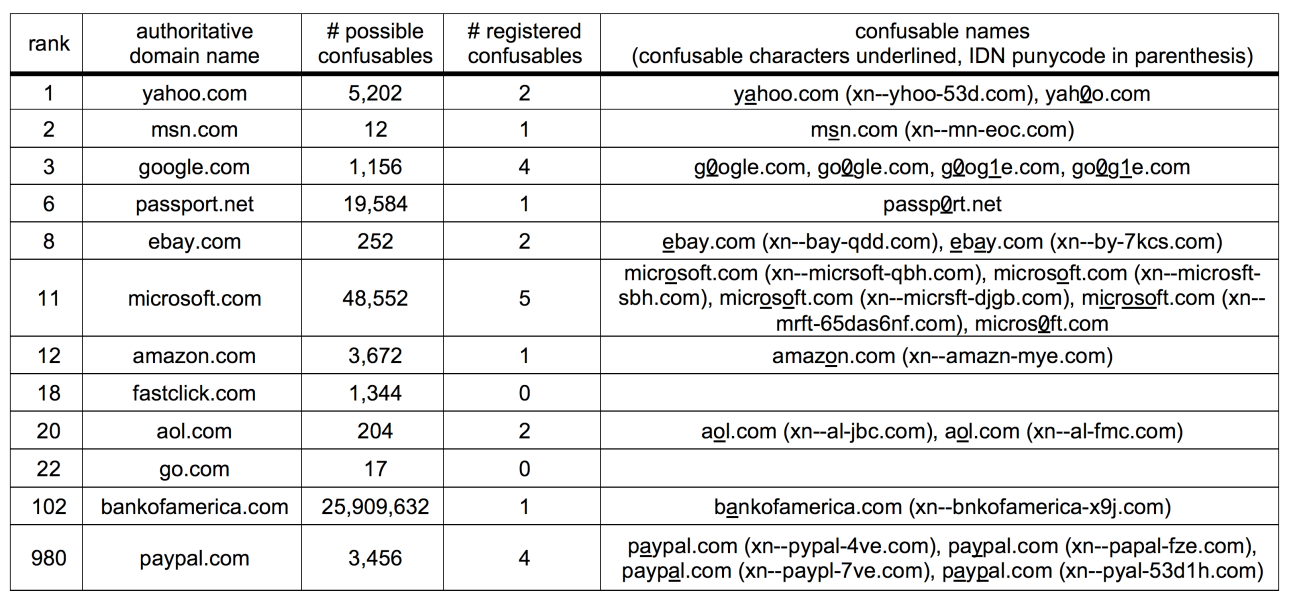
\includegraphics[width=1\linewidth]{evaluation/confusable.png}
    \caption{Registered confusables for popular domains}
    \label{fig:figureAlot1}
\end{figure}

\subsection{ Real-life Mitigations}

The following scenarios are examples of real-life confusable domain mitigations :

\begin{itemize}
    \item \textbf{Cloudflare's Zero Trust Services Approach :} Protection from this problem of newly created phishing websites is given by Cloudflare itself with its protection in the form of Zero Trust services, finding these websites, and blocking confusable domains. Cloudfare zero-trust rules can be enforced using Cloudfare Gateway in a way that they deny access to these illegitimate domains. In such a way, corporate networks are supposed to be secured from phishing attempts that take advantage of human trust in well-known brands \cite{Cloudflare2023}. Cloudflare's Zero Trust services enable a proactive approach to blocking confusable domains, which are important to avoid serving phishing sites. In particular, this mitigating measure will be triggered on the first query that involves any domain that is made through the 1.1.1.1 DNS resolver. Such queries will be inspected by the system and checked against a list of possible phishing domains through a “fuzzy” matching protocol. If the domain matches any of the saved patterns for legitimate brands, then Cloudflare's service would throw an alert. This method used by the server ensures that any domain trying to impersonate a known or respectable brand is detected as soon as it happens in which it provides both real-time monitoring and the capability to search into a historical archive of those domain names, by notifying a security team about new domains observed during the last 30 days that match their saved patterns. This enables a direct review and instant additional taking actions by this domain. The system can also be utilised by Cloudflare for a special investigation in a one-time domain search for some specific domain or pattern, which might become potentially dangerous from a security point of view.

     \item \textbf{IDN Handling of Google Chrome: } Google Chrome enforces an IDN (Internationalized Domain Names) policy to determine which form the Unicode or punycode form a domain label should be displayed in. The domain label is tested to determine whether it has mixed script, invisible characters, or visually confusable characters, and whether it is actually validly converted to Unicode. For instance, domains containing characters of different scripts, or those that are clearly identified as mixed script confusables, will be displayed in punycode, warning the users of potential deceptions. Chrome further offers comprehensive warnings to secure URLs that appear to be an imitation of already known web pages. \cite{ChromiumIDN}
     
\end{itemize}

In addition to what I mentioned above, let us look at the most popular mitigations used world-wide :

\begin{enumerate}
 
  \item Typo-squatting Detection Tool: Tools such as DNStwist and URLCrazy are used to offer organizations similar domain names so that they can either secure these domain names in advance or file litigation for the same.
  \item Anti-Phishing Working Group (APWG): It is a pool for stakeholders to share intelligence, trends and best practices regarding phishing and similar threats associated with confusable domains in which mitigation is carried out in collaboration action between cybersecurity entities and domain registrars, as it allows sharing of threat intelligence with respect or cancelling out the holding of malicious domains.
\end{enumerate}

\subsection{Collaboration Among Registrars, Registries, and DNS Collaborators}

This collaboration should be achieved with DNS registry, registry and collaborators. In that way, they can boost common resources and intelligence that can guide in making the internet more secure and resilient. This strictly falls within the remit of registries and registrars acting in collaboration to put in place such stringent registration policy with procedures for verification, checking against mimicking existing trademarks or even popular domain names.

In this way, the collaboration can even manifest itself via the sharing of sensitive data with regard to domain abuse threats and trends. Databases and threat intelligence platforms are shared amongst stakeholders, allowing them to anticipate and avert most such perils well before they impact netizens. This collective effort will enable the formulation of standards by which to coordinate responses to confusable domain incident reports. Mitigating confusable domains demands that registrars, registries, and DNS collaborators work in a common effort. This is due to the increasing level of threats and the shared responsibility of all actors involved in the DNS ecosystem. \cite{Catania2022} To put this into perspective, here are some examples: 




\begin{enumerate}
  \item Recent changes in the contract from ICANN's contracted parties have imposed on registrars and registries new specifications to define DNS abuse, together with clear requirements for the actions to be taken by such parties immediately actionable evidence of abuse is received. This is a major step towards establishing more clarity about the roles that may be played by these different stakeholders in addressing the matter of DNS abuse and ensuring there is a common approach to redress. \cite{Weinstein2023}
  \item Approved new obligations of ICANN's contracted parties have been by the community itself further to mitigate DNS abuse, thereby demonstrating the will of the community to come together to address the issues of DNS abuse. \cite{ICANN2023}
  \item Efforts like NetBeacon, with the support of the DNS Abuse Institute, are being rolled out to reduce friction in reporting and mitigating DNS abuse. This service solves the current complexities and quality standards associated with the reporting of DNS abuse as it makes the work easier for the registrars, ultimately narrowing down their scope to the relevant and evidenced report as well as it underlines the need for cooperation among registrars, registries, and other DNS stakeholders. This is what is capable of saving the Internet and safeguarding at the same time the credibility and confidence of DNS. \cite{NetBeacon}
  
\end{enumerate}

Real-life examples of entities seeking to block the resolution of DNS names, especially in connection with public recursive DNS servers, frequently revolve around matters of control, filtering, or securing internet traffic with various kinds of motivations corresponding to such sectors. Some attempted these efforts at the governmental, corporate, and individual levels. As typical examples that pinpoint those instances, consider:

\begin{enumerate}
    \item Governmental Efforts to Block DNS Resolutions : Governments may interfere directly in the DNS operation to enforce some censorship or block access to particular types of content. For instance, China uses the Great Firewall for regulation concerning access to the World Wide Web within their territory, including doing some mishandling connected with the DNS in order to block out unwanted content. \cite{XuAlbert2017MediaCensorship}
    \item Corporate and ISP DNS Filtering : DNS filtering can be deployed by companies and even ISPs in a bid to achieve enhanced online security. For instance, Heimdal Security explicates how the DNS filtering works as one of the measures for preventing their access to various harmful or inappropriate websites since it first checks the requests for domains. If some are actually flagged, access is denied, hence maintaining both security and productivity within one's organization. This approach is really very effective for the prevention of phishing and malware attacks because it stops the DNS requests towards the malicious sites. 
    \item Ad Block DNS Services :  Cloudflare discusses how DNS filtering can be used to prevent access to malicious sites and also filter what is harmful or unfit for viewing. This is done at the DNS level so as to prevent these sites from loading on devices. Cloudflare uses its DNS to filter part of a more prominent policy of access control—an effort to secure company data and govern what employees will see on the network they manage.    
\end{enumerate}

 On the negative side, attackers are taking advantage of DNS blocking mechanisms to perform DNS-based attacks. These include using DGAs (Domain Generation Algorithms) for malware communication, using FastFlux techniques for slipstreaming attacks, basically creating malicious newly registered domains (NRDs) that appear benign and legitimate to an outside observer, etc. All this makes it difficult to block bad content at the level of DNS, which calls for quite sophisticated countermeasures.


\subsection{Techniques for Mitigating Confusable Domains}

Mitigating confusable domains requires sophisticated techniques tailored to address the unique challenges presented by both non-Internationalised Domain Names (non-IDNs) and Internationalized Domain Names (IDNs). This differentiation is significant  due to the distinct nature of threats they pose and the technical feasibility of the mitigation strategies applicable to each. The following is a detailed examination of mitigation techniques, along with discussions of the operational feasibility and potential collaboration frameworks involved.

Non-IDNs Mitigation Techniques : Strategies focus on identifying and mitigating domain squatting and typo-squatting, where attackers register domains that are typographical errors or close variants of legitimate domains to deceive users.

\begin{enumerate}
  \item Registry-Level Measures: Domain registries can implement checks to prevent the registration of domains that are similar to the existing trademarks or brand names, using algorithms to detect variations and misspellings closely resembling protected names. \cite{WTR2020} 
  \item Trademark Protection Programs: Services like the Trademark Clearinghouse (TMCH) offer mechanisms for trademark holders to protect their rights by receiving notifications when someone attempts to register a domain matching their trademark. \cite{ICANNTMCH}
  \item Automated Monitoring and Reporting: Automated systems can continuously monitor domain registrations for names that closely resemble known trademarks or brand names, enabling rapid detection and legal action against infringers. \cite{TMCH2023}
\end{enumerate}

IDNs Mitigation Techniques : The challenge with IDNs lies in the potential for homograph attacks, where attackers use characters from different scripts that appear visually like characters in the Latin script to create deceptive domains.

\begin{enumerate}
  \item Punycode Awareness and Monitoring: Web browsers and security tools convert IDNs to punycode, a representation that encodes the Unicode characters in ASCII. Awareness of punycode and monitoring for suspicious registrations can help identify potential homograph domains. \cite{SOCRadar2023}
  \item Browser-Level Defenses: Modern web browsers have implemented defences against IDN homograph attacks by displaying the punycode version of the domain or alerting users when a domain name contains characters from multiple scripts. \cite{Malwarebytes2017}
  \item Collaborative Blacklisting and Sharing of Threat Intelligence: Organisations can collaborate to share intelligence about known malicious IDNs, contributing to comprehensive blacklists that can be used by registrars, DNS providers, and end-users to block access to malicious sites. \cite{CyberThreatAlliance2023}
  
\end{enumerate}


However, ICANN plays a pivotal role in the detection of confusable domains as it detects confusable domains, especially with respect to Internationalized Domain Names (IDNs) but also it doesn't provide a direct list publication on confusable domain, just like the other gTLD registries. Instead, they tend to develop the frameworks and guidelines for managing the threats related to IDNs and name collisions. This will involve the development of protocols regarding how the processing of internationalized domain names would be done and how the impact that name collisions may possibly have on the domain name system is minimized. \cite{ICANNIDNs}

People detect on-Internationalized Domain Names (non-IDNs) and Internationalized Domain Names (IDNs) using comprehensive domain, IP, and DNS intelligence tools. Tools which can do so, such as those offered by services like the WhoisXML API, help check domain names for the presence of suspiciously similar domains that could potentially confuse or deceive consumers. An IDN deceptive score is given by means of an algorithm to such types of domains that take into account visual similarities, brand names, and TLD features to see if a domain name is being prepared for deceptive purposes. This approach has proven to be effective in academic research projects at identifying deceptive IDNs over millions of domains distributed across various top-level domains. \cite{WhoisXMLAPI}

\subsection{Technical and Operational Feasibility}
The technical feasibility of these techniques varies. Registry-level measures and trademark protection programmes are quite effective, but require cooperation and standardisation across different legal jurisdictions. Automated monitoring is technically feasible and can be implemented on a scale but requires resources for continuous operation and legal follow-up. Browser-level defences are among the most directly impactful, protecting users at the point of access, yet they depend on browser vendors' willingness to implement and maintain these features, and collaboration frameworks play a crucial role in mitigating confusable domains. Initiatives such as the Trademark Clearinghouse (TMCH) facilitate cooperation between trademark holders and domain registries. Meanwhile, organisations such as the Anti-Phishing Working Group (APWG) and the Internet Corporation for Assigned Names and Numbers (ICANN) work toward broader solutions that encompass both non-IDNs and IDNs.

\subsection{ Transparency in Mitigation Efforts}

Transparency in the mitigation of confusable domains plays a pivotal role in the broader strategy to secure the Internet against phishing attacks, trademark infringement, and other malicious activities. This concept entails the practices adopted by domain registries and registrars in identifying potentially malicious domains that mimic or closely resemble legitimate ones, and the extent to which these entities disclose identified confusable domains to the public. One of the primary methods to improve transparency involves the publication of lists of confusable names by registries and registrars. These lists typically include domains flagged for their similarity to existing domain names, potentially infringing trademarks, or those that could be used for malicious purposes. The publication aims to alert the internet community, including businesses and end-users, about possible threats, thereby fostering a proactive approach to domain name security. Here is how transparency can be applied to each of the mitigation techniques described:

\begin{itemize}
  \item \textbf{Cloudflare's Zero Trust Services Approach: }Cloudflare's process for identifying and blocking confusable domains should be transparent to its users. This includes detailing the criteria for flagging domains as phishing sites and the mechanisms in place for users to appeal or request a review of blocked domains. By openly sharing the methodology behind their zero-trust rules and how they are applied through the Cloudflare Gateway, trust in Cloudflare's protective measures is bolstered among corporate networks.
  
  
  \item \textbf{IDN Handling of Google Chrome:} Google's approach to displaying domain names in Unicode or punycode based on their potential for deception benefits from transparency about its IDN policy. Detailed explanations of the checks performed (e.g., mixed script detection, invisible characters) and how decisions are made improve user understanding and awareness of potential threats. Furthermore, publishing information on how users can report misclassified domains or suggest improvements to the IDN policy can further empower users and foster a safer Internet environment.
  
  
  \item \textbf{Typo-squatting Detection Tools: }The effectiveness of tools like DNStwist and URLCrazy in helping organizations identify potential confusable domains relies on transparency about how these tools generate similar domain names and the criteria used for detection. Openly sharing updates, methodologies, and case studies can help organisations better understand how to use these tools proactively.
  
  \item \textbf{Collaborative Efforts and Intelligence Sharing: }The partnership between cybersecurity entities and domain registrars, as well as initiatives such as the Anti-Phishing Working Group (APWG), should prioritise transparency in their operations. This includes the sharing of methodologies for threat detection, the criteria for taking action against malicious domains, and the processes for stakeholders to contribute or access shared intelligence. Transparency in these collaborative efforts ensures that actions taken against confusable domains are fair, understood by all parties involved, and supported by a broad community of internet security stakeholders.
  
 \item \textbf{Transparency for non-IDN registries : } 

 \begin{enumerate}
  \item Registry-Level Measures: Transparency in level-registry measures becomes a necessity if trust has to be kept between registrants and domain trademark owners. They are published criteria and algorithms used to find variations and misspellings of the names submitted for protection. Making these publicly available can then ensure fairness and feedback in detecting mechanisms is therefore paved for improving them.
  \item Trademark Protection Programs: Services such as those from a Trademark Clearinghouse (TMCH) should operate with full transparency regarding the conductance of verification, matching, and notification. This can help trademark holders by demonstrating transparent guideline procedures that show both the rights of trademark holders and what needs to be done to effectively protect their brands.
  \item Automated Monitoring and Reporting: The automated monitoring systems must be built with such predefined criteria, algorithms, and thresholds that potentially support the involvement of stakeholders. It also makes sure that the brand owners are aware to what extent his trademarks are protected, and thus allows for some parameters within such services making the monitoring more successful.
\end{enumerate}
 
 \item \textbf{Transparency for IDN registries  : } 

  \begin{enumerate}
  \item Monitoring and Identifying Measures for Suspicious Punycode Registrations: All domain registrars and trademark owners, together with security professionals, must adhere to measures on suspicious punycode registrations. Publicising the details of activities carried out to monitor them propagates homographic threats through collective ideas, also in their identification and mitigation.
  \item Browser-Level Defences: A good web browser should play the most critical role in defending against IDN homograph attacks. Browsers must document, provide, and communicate their defence mechanisms in a clear and plain manner to users. For instance, they should indicate when a domain is being displayed in puny code or the scenarios under which their warnings are triggered. This can only give a user assurance if there is transparency as a rationality measure for them in such defence measures to be able to rationalize the triggering of any warning and know what action to take.
  \item Collaborative Blacklisting and Shared Threat Intelligence: Processes for the addition of domains to blacklists and criteria that determine whether a domain is to be considered malicious should be examined. Organisations that put in place an intelligence sharing regime also need to have some rules on data submission and validation and data disposal from blacklists. Transparency in these processes can best ensure that blacklisting is done fairly and accurately and allows the right of appeal, improving trust in collaborative security.
\end{enumerate}
  
  
\end{itemize}

In summary, transparency across all these mitigation techniques not only builds trust among users, developers, and organizations but also enhances the collective ability to respond to and prevent the threats posed by confusable domains.

\subsection{Benefits of Transparency }

The benefits of transparency in the context of confusable domains are multifaceted. Firstly, it promotes accountability among domain registrars and registries, encouraging them to actively participate in the detection and mitigation of confusable domains. Second, transparency acts as a deterrent to malicious actors who might otherwise exploit the anonymity afforded by a lack of public scrutiny. Third, by making such lists public, registries and registrars can empower businesses and trademark owners to take timely action to protect their brands, such as through legal mechanisms or domain purchases. Furthermore, transparency supports community-based mitigation efforts, where cybersecurity researchers and the wider community contribute to identifying and neutralizing threats. This collaborative approach leverages the collective expertise of the cybersecurity community, enhancing the overall effectiveness of mitigation strategies.

\subsection{Drawbacks and Security Concerns} 

However, the publication of confusable domain lists is not without its drawbacks and security concerns. One major concern is that making such lists public could inadvertently provide a roadmap for malicious actors, highlighting potential targets for exploitation. This could lead to a situation where attackers use the information to refine their strategies, for example, by registering domains not yet identified or listed, thereby staying one step ahead of mitigation efforts. Another concern revolves around the risk of false positives, where legitimate domains are mistakenly flagged as confusable. This could harm businesses and individuals whose domain names are wrongfully listed, potentially leading to unwarranted scrutiny, legal challenges, and reputational damage. Moreover, the debate between transparency and security also touches on the effectiveness of disclosure in preventing attacks. While transparency aims to preemptively combat threats, there is an argument that the sheer volume of domain registrations and the dynamic nature of domain abuse may limit the practical utility of such lists to end-users and businesses.

\subsection{ Analysis : Feasibility and Practical Challenges}

 \begin{enumerate}
  \item Automated Monitoring and Reporting: Feasible; Technology exists to automate monitoring, even though the refinement of algorithms to decrease false positives and negatives from human review can probably not be undertaken with existing resources.
  \item  Monitoring Punycode Registrations: Feasible; This option is feasible and will require mainly the use of existing technology and cooperation that could be initiated with little difficulty between relevant stakeholders.
  \item Blacklisting and Threat Intelligence Sharing: Moderately Feasible; Since agreement could be reached on shared platforms and protocols, but they imply strong cooperation and trust among such diverse entities, which is unlikely to be developed fast.
  \item Registry-Level Measures: Not Feasible; this would require very heavy coordination and agreement on standards across diverse jurisdictions and registries, very complex in nature and long-drawn.
  \item Trademark Protection Programs: Moderately Feasible; They are well-functioning processes under such adequate structures like TMCH and can be learnt while proceeding with experience, but likely to face legal and operational issues.
  \item  Browser-Level Defences: Not Feasible; While this is technically feasible, it seems rather infeasible soon that user practices will become uniform across all web browsers and that all users will be well trained in various security practices.
  \item Cloudflare's Zero Trust Services Approach: Feasible; since well-architected infrastructure and broad adoption have made Cloudflare zero-trust rules simple and effective to deploy, with a balance of security and operational efficiency without seismic root and branch changes.
  \item IDN Handling of Google Chrome and Browser-Level Defences: Feasible; Given that Chrome today has an enormous user base and that the groundwork for stopping homograph attacks already exists, it stands to reason that a solution is reasonably possible, meaning not too difficult, within a set timeline, and within the lifespan of any other typical software product.

  
\end{enumerate}

\section{Phishing}

\subsection{Real-life examples}

Phishing, a cybercrime in which targets are contacted by email, telephone or text message by someone posing as a legitimate institution to lure individuals into providing sensitive data, has become increasingly sophisticated. Two notable examples include :

\begin{enumerate}
    \item InterMed and Spectrum Healthcare Partners fell for a major phishing attack on 44,000 patient data. A Portland-based health care provider, InterMed, could have put the security of 33,000 protected health information (PHI) of its patients at risk due to an attack detected on September 6. Attackers were in the system from September 4 through September 10. The compilation of revealed information included and was not limited to names, dates of birth, health insurance information, and even clinical information accompanied with exposed social security numbers in some cases. In other data breached, Central Maine Orthopaedics issued a report that affected 11,308 patients within their service area by the Spector Healthcare Partners group. Obviously, unauthorized access to emails gives some glimpses about their patient names, date of birth, addresses, and clinical information. This is truly a bad reflection in the middle of an upswing of threats towards health data security, and thus, peremptory steps are required, not just in respect of strengthened security of emails, but in the deep training of support professionals in the best practices \cite{HIPAAJournal2020Phishing} .
    \item In a breathtaking cyber fraud case, both Google and Facebook were almost swindled out of nearly \$ 100 million each via increasingly advanced phishing attacks in less than two weeks. In fact, the fake emails were near-identical replicas of real invoices that had been sent by actual suppliers, such that trust and daily procedures were abused in making huge money transfers to fraudster-controlled accounts. This incident is only a portrayal of how susceptible research firms which are highly developed technologically are in the hands of social engineering and thus calling for the tightening of security measures, constant training of the employees, and verification of threats that have evolved in the cyberspace \cite{CNBC2019Phishing}.
\end{enumerate}

\subsection{Real-life Mitigations} 

\begin{itemize}
    \item \textbf{Employee Awareness and Training :} Very affirmative in the number of ways a phishing activity is carried out, and the training programme prepared through simulation scenarios for the employees, the Chelsea Technologies employee education policy can be said to be the most significant. It is an inevitable approach, as in most cases, employees contain the credentials and knowledge that drive the breach to succeed. Bringing employees up to date on the different methods of phishing, for example, spoofs and malicious attachments, arms them well in the guarding of sensitive information \cite{DigitalGuardianPhishingPrevention}.

     \item \textbf{Comprehensive Security Measures: } LaptopMD points out that the risk of ignorant searching requires the formulation of policies that make it difficult to land on some sites. Besides this, the awareness on the phishers techniques and browsing issues by employees will greatly save them from being caught in cases of phishing \cite{DigitalGuardianPhishingPrevention}.
     
     \item \textbf{Technological and Human Factors: } Each SecureHIM security approach comes with layers of added security in between these, from technological tools such as spam filters and two-factor authentication to staff. It identifies the suspicious link, abstains from clicking on it, and maybe even some browser add-ons that allow one to easily skip some dangerous links. This underscores the fact that technological peripherals and informed employees are crucially needed to provide an effective defence against phishing attacks \cite{DigitalGuardianPhishingPrevention}.

     \item \textbf{Awareness against unsolicited emails:  } The Center for Democracy and Technology (CDT) outlines some of the best practices in the recognition and act to mitigate phishing; they include the sense of making urgent and unsolicited emails with poor headers, poor links, refusing to reply, open or to click on anything. The next emphasis is to train users on the awareness of phishing by setting avenues for reporting all suspicious messages \cite{CDTPhishingMitigation}.
     
     
\end{itemize}

\subsection{Techniques for Mitigating Phishing}

Current phishing attack mitigation techniques focus mainly on preventing phishing
emails from reaching the users’ inboxes and on discouraging users from accessing
phishing websites \cite{Suzuki2021Phishing}.

\begin{enumerate}
    \item Email Filters: Advanced algorithms are used to identify phishing emails on the basis of a predetermined set of attributes, such as the reputation of the sender, links embedded in the body of the email, and keywords flagged as associated with phishing are prevented from reaching the inbox.
    \item Domain blocking: The first step at an organisational level to make the phishing site not openable by users accidentally is applying domain-blocking measures whether access to the known phishing website from inside an organisation network, this usually inhibits access.
    \item User Training: It is important that users are trained directly and to be reminded of any danger they are facing. Training users will require development along the lines of sensing signs in phishing emails, risk taking such as clicking on unknown links, or giving away personal or sensitive information.
\end{enumerate}

The introduction of Situational Crime Prevention Approach (SCP) \cite{Suzuki2021Phishing}, which is an idea about understanding the detailed offender thought process and the attributes in the environment allowing the attack. This approach looks to deter potential attackers simply through raising the level of effort and risk involved in an attacker conducting a successful phishing attack with concomitant reduction in the likely rewards. This method underscores the importance of understanding the criminal's perspective and creating a hostile environment for phishing activities through strategic preventive measures. This method involves these steps : 

\begin{enumerate}
    \item Increasing the Effort for Attackers: Implementing strong authentication methods and encryption to make it more challenging for phishers to access or spoof legitimate websites or email accounts.
    \item Clarifying Users' Responsibilities: Educating users about their role in maintaining cybersecurity, including recognizing phishing attempts, and reporting them.
    \item Enhancing Detection Probability: Utilizing advanced detection technologies and threat intelligence to identify and neutralize phishing threats promptly.
    \item Limiting Phishers' Access: Restricting the amount of publicly available information that could be used for crafting convincing phishing emails or impersonating individuals or organizations.
    \item Discouraging Future Attacks: Implementing punitive measures against identified attackers and sharing information about phishing campaigns with broader communities to prevent repeat offenses.
\end{enumerate}

This measure is not only designed to stop a phishing attack but rather to create an environment that would lead the cost-benefit ratio for phishing not so appealing to the attackers. In fact, comprehensive perspectives in addressing phish through the three methods above singularly go to dramatically lower the vulnerability of organizations and individual persons to such acts.

In addition, Phishlimiter \cite{Chin2018PhishLimiter} which is a new phishing detection and mitigation approach using Software-Defined Networking where it first proposes a new technique for deep packet inspection (DPI) and then leverage it with software-defined networking (SDN) to identify phishing activities through e-mail and web-based communication.This is how it works :

\begin{enumerate}
    \item Deep Packet Inspection (DPI): Analyses the data part of network packets beyond basic header information. It inspects the content of packets for signatures and patterns associated with phishing.
    \item Store and Forward (SF) and Forward and Inspect (FI) modes: SF mode temporarily stores packets for thorough inspection before forwarding, while FI mode prioritizes immediate forwarding with parallel inspection to reduce latency.
    \item Artificial Neural Network (ANN): A machine learning model that classifies network traffic to identify potential phishing activities by learning from known phishing signatures and behaviours.
    \item Dynamic adjustment of network flows: Upon detection of a threat, the system dynamically reroutes or restricts traffic to mitigate potential phishing attacks, adapting to new threats in real-time.
    \item Minimal disruption to network services: Designed to ensure that the phishing mitigation process does not significantly impact network performance, ensuring smooth operation of network services even under threat detection and mitigation activities.
\end{enumerate}

\subsection{Transparency in Mitigation Efforts}

Transparency in cybersecurity, including phishing mitigation techniques, refers to how openly and clearly the methods, policies, and procedures are communicated, understood, and accessible to all stakeholders involved, particularly employees. Here's how transparency can be applied to each of the mitigation techniques described:


\begin{itemize}
    \item \textbf{Employee Awareness and Training :} 
    
    Communication: This will consist of clear informing of the employees on the kind of threat and how it could mean for the organization and their role in these defences.
    
Accessibility: Make people aware that the repository exists, or make the resources easily available for reference. This would include an intranet site or a repository where people could easily access the trending practices in phishing on the latest and how to respond.

Having a clear and simple method will inspire the employees to report the false phishing attempts and express their opinions on the training program. It encourages active participation and continuous improvement in the training material.


     \item \textbf{Comprehensive Security Measures: }
     
     Policy Publishing: All available policies, notably those pertaining to web browsing, email attachments, and use of security tools, will be published in open sight to let employees know about them.
     
Justifications: The rationale behind specific policies, and restrictions so that the employee will appreciate why they are being put in place, does not appear to be a set of arbitrary rules.

Changes and Updates: Introduce the workforce to changes relating to security measures and how such changes are beneficial and serve as a cover against new hazards

     \item \textbf{Technological and Human Factors: } 
     
     Tool Transparency: Clearly state the tool and the reason for its being in place for security (e.g., spam filters, two-factor authentication), and its work on subduing phishing. Doing so, such technologization should ideally demystify lay trust in these systems.
     
User Control and Visibility: Attempt to give the users some form of control or visibility over the security tools, through which their work could be affected. Feedback from a blocked phishing attempt could, for example, help to reinforce the training.

A Continuous Feedback Loop: Reports and discussions of not only the phishing attempts that technology catches, but also of the ones it misses, have to be actively tracked in order to keep the human element alive in cybersecurity.


     \item \textbf{Awareness against unsolicited emails:  } 
     
     Open Communication on Threats: Constant update on new phishing techniques and any other notable attack are discussed among the industry for them to be updated.
     
Best practices: develop best practices for easy identification and to be visible on how to catch and react to phishing attacks, with graphic examples or checklists.

Development of Trust: Create an environment where employees will not have any fear of revenge for reporting any insecurity that they might suspect. This can be enabled by an easily established reporting system that is anonymous.
\end{itemize}

\subsection{Analysis : What is feasible }

\begin{enumerate}
    \item Employee Awareness and Training : Feasible; Regular training and simulation exercises can be implemented across organisations of any size with scalable online platforms, requiring minimal resources beyond the initial setup.
    \item Comprehensive Security Measures :Feasible; The deployment of web filters and secure browsing policies is technically straightforward with existing technology. The main effort lies in continuous policy update and employee education.
    \item Technological and Human Factors: Feasible; The integration of spam filters, two-factor authentication, and secure browsing add-ons is readily achievable with current technology. The human element—ongoing employee vigilance—enhances the effectiveness of these tools without significant additional costs.
    \item Awareness against unsolicited emails: Feasible; Establishing and communicating best practices for handling suspicious emails involves minimal costs and leverages existing communication channels within organizations.
\end{enumerate}

\chapter{Conclusion}

\section{Brief Review}

This project looked at DNS abuse, a situation in which malicious actors exploit domain names for malicious activities such as phishing. DNS infrastructure providers, including registrars and registries, have been the focal points of attention due to their significant roles in controlling and potentially reducing this abuse. The investigation included the complaints these providers receive and the measures they take to mitigate abuse, such as the deletion or blocking of domain name registrations. A critical aspect of this research was the concept of transparency: the extent to which these actions are disclosed and documented by the providers. It was found that the practice of issuing comprehensive transparency reports is not as widespread as necessary, despite the crucial role that openness plays in fostering trust and accountability in the digital realm. 


\section{Main Results}

\subsection{Related back to Project Objectives:}

The project led to the identification of serious transparency gaps in the mitigation of DNS abuse adopted by infrastructure providers. Although some reporting and communication measures of mitigation action against DNS abuse have been embraced to trace the information on the mitigation measures undertaken, it is largely inconsistent. This goes hand in hand with our first objective, to further understand practices on transparency in the area and set a clear requirement for standardised transparency measures.

\subsection{Summary of Proposals:}

Throughout the research project, a number of strategies for improving transparency have been discovered:


\begin{enumerate}

    \item Regular Transparency Reporting: Urge all DNS infrastructure providers to release reports on a regular basis describing the steps they have taken to mitigate DNS abuse.

    \item Stakeholder Engagement: Encourage more cooperation and communication on transparency regulations between DNS providers, users, and legislators.

    \item Public Accountability Mechanisms: Provide and implement systems that let the general public monitor and evaluate DNS abuse mitigation efforts.
    
    \item Innovation in Defence Strategies and Sharing: Emphasise the importance of preparing new methods to combat DNS abuse by developing and encouraging the sharing of these innovative strategies among stakeholders.
    
    \item Transparency in Monitoring and Collective Action: Encourage open observation of DNS activity and cooperative efforts from all parties within the DNS ecosystem to guarantee a unified strategy for mitigating abuse.
    
\end{enumerate}

These strategies seek to expand on the fundamental measures outlined in this research project, focussing not just on the individual efforts of DNS infrastructure providers but also on the collective efforts and shared responsibilities throughout the DNS ecosystem. By using these tactics, the internet community can work towards improving trust and transparency, which will result in a DNS system that is more secure and resistant to abuse.


\subsection{Assessment of Contribution :}

These results can be used to show the importance of the application, as the responsibility may fall on the DNS infrastructure providers to have a better and more transparent practice in mitigating DNS abuses. Eventually, the adopted strategies give a chance for better accountability and more trust from the interested users and parties. In the larger context of cybersecurity and internet governance, where transparency is becoming more widely acknowledged as essential to promoting a safer online environment, this contribution is vital.


\section{Future Work}



\subsection{Further Research Directions:} Future research should examine how AI and machine learning are combined to detect predictive DNS abuse and how well international regulatory frameworks enforce transparency requirements. In addition further research may examine how user trust and behaviour are affected by transparency, as well as how various degrees of openness influence how DNS infrastructure providers are seen. Additionally, studies could assess how well different transparency techniques mitigate DNS abuse in the real world.

\subsection{Practical Next Steps for Developing Transparency Best Practices: }

\begin{enumerate}
    \item Framework Development: Collaborate with leading industry players to develop a uniform transparency framework that DNS infrastructure providers can use anywhere.

    \item Technology Solutions: Looking into technical options that automate the gathering and sharing of DNS abuse data to improve transparency.

    \item Policy Recommendations: Draughting policy suggestions should require transparency in these activities to encourage legislative support for DNS abuse mitigation initiatives.
    
    \item Stakeholder Collaboration: Governing bodies that maintain DNS infrastructure, regulatory organisations, and cybersecurity communities need to join hands to combat and find an amicable solution to these challenges.
    
    \item Transparency Standardisation: Standardise transparency reports across the industry to ensure uniformity in disclosing DNS abuse mitigation efforts.
    \item Real-Time Monitoring: Implement real-time abuse monitoring dashboards to enable swift detection and response to DNS threats.
    \item  Public Awareness: Promote user education on DNS security to enhance public awareness and safeguard against potential abuses.
\end{enumerate}


\subsection{Enhanced Transparency Practices for DNS Abuse Mitigation: }

Building on these initial steps, registries and registrars are urged to implement improved transparency measures such as the following to strengthen the DNS ecosystem's resistance to abuse:

\begin{enumerate}
    \item Public Reporting: Establish thorough and consistent transparency reports that provide information on the number of DNS abuse reports received, the steps taken, and the results of those steps. In addition to increasing user trust, this transparency makes the organisation responsible for efficient abuse mitigation.

    \item Stakeholder Engagement: Provide forums or advisory committees to discuss and evaluate mitigation solutions for DNS abuse that involve a wide range of stakeholders, such as government representatives, cybersecurity professionals, and members of civil society. This guarantees that decision-making procedures take into account a wide range of points of view.

    \item Abuse Point of Contact: Clearly identify the abusive contact and make it public. This makes it easier for the community, including end users and cybersecurity researchers, to report and handle abuse problems effectively.

    \item Best Practice Sharing: Encourage an environment of transparency by sharing best practices, resources, and innovations for mitigating DNS abuse to colleagues in the DNS ecosystem. Workshops for the entire industry or collaborative platforms can help to promote this conversation.

    \item User Education:C reate and distribute instructional materials to help domain owners and end users identify and stop DNS misuse. Empowering people with knowledge can drastically reduce the effectiveness of phishing and other abusive techniques.

    \item Automated Abuse Detection: Make use of AI and machine learning technology to automatically identify possible DNS abuse behaviours. Exchange anonymous indicators of compromise (IoCs) with reliable partners to increase the resilience of the ecosystem as a whole.

\end{enumerate}


\subsection{Future Directions in DNS Abuse Mitigation: }

Future studies and practical initiatives should focus on the following areas to better address the dynamic nature of DNS abuse and proactively counter new threats:

\begin{enumerate}
    \item Emerging Technologies: Exploring the possibility of DNS abuse and creating focused mitigation solutions in AI-generated content and the growth of IoT devices.

    \item AI and Machine Learning for Proactive Defence: Using data analysis to find possible abuse vectors and advancing AI and machine learning models to anticipate and handle DNS abuse before it happens.

    \item Enhanced IoT Security: Establishing security guidelines for IoT device makers to stop device exploitation in DNS abuse, encouraging industry-wide adoption via partnerships and laws.

    \item Global Policy and Regulation Dialogue: Participating in policy discussions to coordinate mitigation measures for DNS abuse and promote laws that promote security, privacy, and openness.

    \item Transparency Evolution: Advancing transparency standards in line with technology, emphasising real-time data sharing, blockchain-based log reporting, and user-friendly interfaces to prevent unauthorised access to data.

    
\end{enumerate}


\subsection{Contributions to Future Transparency Practices:}

This research contributes to the ongoing development of best practices for transparency in DNS abuse mitigation.By emphasising the significance of transparent, consistent reporting and promoting stakeholder interaction, it seeks to enable better informed policy-making and promote a safer online environment. Identifying existing challenges and proposing feasible solutions, this study is a first step towards improving openness in the DNS ecosystem. The desired results are a reduction in DNS abuse, an informed and active user base, and the development of a more reliable Internet ecosystem.


\section{Reflection}
\subsection{Personal Learning: } 

With this project, I have appreciably learned the complexities of DNS abuse  and how these complexities might pose a challenge in coming up with systems that address the potential lack of transparency. In that sense, DNS abuse is said to be very dynamic, always changing to expose new tactics by bad actors; mitigation strategies should, therefore, become adaptive.  I learnt that transparency isn't just about sharing information; it is about building trust within the community, improving the effectiveness of abuse mitigation efforts, and impacting broader internet governance and security positively.

\subsection{Evaluation of Research Process:  }

In other words, this research project has brought to light the complicated hurdles in studying DNS abuse mitigation transparency, from the reluctance to share sensitive information due to privacy and security concerns to possible biases in data self-reporting. The process made clear the delicate balance that must be struck between maintaining security and releasing just enough information to be transparent. Although the technique made it possible to conduct a thorough analysis, it also highlighted areas that needed to be improved, such as determining more accurate ways to assess how transparency practices affect the reduction of DNS abuse.



\subsection{Perspective on Research Findings and Contributions: }

This research project offers a more comprehensive view of current procedures and their effectiveness, contributing to continuing conversations on DNS abuse mitigation and transparency. Through gap analysis and practical strategy recommendations, the study highlights the necessity of a coordinated approach to openness. It calls for the creation of guidelines and best practices that improve cooperation between all parties involved in the DNS ecosystem. While great progress has been made, my work emphasises the ongoing need for attention and effort in this area and suggests that the road towards a more transparent, safe, and abuse-resistant DNS landscape is far from over.


In summary, this project has improved my knowledge of DNS abuse mitigation and the pursuit of transparency, while also providing insightful information that will guide future research in this area of cybersecurity and Internet governance.



\chapter{Findings}
This document provides a template for the preparation of final year project reports. The objective is to provide clear guidance to you, the students, and also to provide uniformity to the project reports, to facilitate equitable grading.
This LaTeX template uses a sans-serif font to aid accessibility..

The font colour for Chapter headings is “Pantone Blue”, which is the colour used in TCD documents. The page number appears at the bottom of each page starting at 1 on the first page of the Introduction chapter.
If you are not familiar with concepts like styles, captioning, cross-referencing, and how to generate tables of contents, figures etc. in LaTeX, the Overleaf guides are a useful start at: \url{https://www.overleaf.com/learn/latex/Learn_LaTeX_in_30_minutes}
\section{Headings, sections and subsections}
Chapters should be divided into appropriate subsections. LaTeX makes the numbering much easier and it is all built in. Headings should incorporate the Chapter number into them as is done here.

\subsection{Subsection name style}
The subsections, if used, should be numbered sequentially within each section.  You should really try to avoid using sub‐ subsections, but if you do they should not be numbered.

\section{Length of the report}
The page margins is set to 2.54 cm top, bottom, left and right. There may be a table or figure for which it is sensible to deviate from these margins, but in general the main text should be formatted within the specified margins.
The body of the report should be organised into several chapters. There are a number of chapters that you must have: an introduction; a background or literature review chapter; and a conclusion chapter. The focus of the other chapters will depend on your specific project. Refer to the issued guidelines for the page limit. This limit does not usually include the front matter, references list and any appendices. In other words, from the first page of the Introduction to the last page of the Conclusions chapters must be less than the given limit for MAI.
If you exceed these page limits or deviate significantly from this format, you will lose marks.
\section{Contents of the Introduction} 
The introduction presents the nature of the problem under consideration, the context of the problem to the wider field and the scope of the project. The objectives of the project should be clearly stated.
\section{Contents of the background chapter}	



% note that your supervisor may have a strong opinion on the style of referencing you use. Some background is available at https://www.overleaf.com/learn/latex/Bibtex_bibliography_styles
\bibliographystyle{IEEEtran} %Changed to IEEETran by HS
%\bibliographystyle{unsrt}
\nocite{*}
\bibliographystyle{plainnat}
\bibliography{bibs/sample}
\appendix
\renewcommand{\thechapter}{A\arabic{chapter}}
\chapter{Appendix}


The Domain Name System (DNS) plays a role in the infrastructure of the Internet by converting user domain names into IP addresses. However, due to its use and importance it has become a target for actors seeking to exploit it. These abuses range from setting up phishing websites to taking advantage of DNS for activities such as typosquatting. The responsibility for mitigating abuse primarily lies with DNS infrastructure providers, such as registrars and registries. These entities respond to reports of abuse by taking down confirmed domain names or proactively blocking the registration of harmful ones. While these actions are essential for maintaining the security and integrity of DNS, they also raise questions about how transparent these measures are. 

Transparency in the context of mitigating DNS abuse refers to the disclosure of actions taken by registries and registrars including the criteria and reasoning behind their decisions. Currently, there is prevalence in publishing transparency reports related to this matter leading to a lack of clarity and understanding about the processes involved in combating DNS abuse. This project aims to address this issue through a survey involving registries, registrars and other stakeholders actively engaged in mitigating DNS abuse.

The main objective of the survey is to collect organise and describe the transparency reports they are presently accessible. This will help us gain an understanding of the status of transparency, in mitigating DNS abuse.

\section{Appendix numbering}
Appendices are numbered sequentially, A1, A2, A3\ldots The sections, figures and tables within appendices are numbered in the same way as in the main text. For example, the first figure in Appendix A1 would be Figure A1.1. Equations continue the numbering from the main text.



\end{document}